\documentclass{article}
\usepackage[margin=2.5cm, includefoot, footskip=30pt]{geometry}

\setlength{\parindent}{0em}
\setlength{\parskip}{1em}
\renewcommand{\baselinestretch}{1}

%%%%Packages%%%%
\usepackage{amsmath}
\usepackage{booktabs}
\usepackage{graphics}
\usepackage{multicol}
\usepackage[ruled,vlined]{algorithm2e}
\usepackage{setspace}
\usepackage{graphicx}
\usepackage{subcaption}
\usepackage{hyperref}
\usepackage{color,colortbl}
\usepackage{array}
\usepackage{booktabs}
\usepackage{tabularx}
\usepackage{wrapfig, blindtext}
\usepackage{soul}
\usepackage[table]{xcolor}
%%%%%%%%%%%%%%%%%

\definecolor{Gray}{gray}{0.92}
\usepackage[first=0,last=9]{lcg}
\newcommand{\ra}{\rand0.\arabic{rand}}

\newcommand{\uniquenumberofseeds}{11400}
\newcommand{\numberofalltournaments}{45606}
\newcommand{\numberofstrategies}{195}
\def\axelrod{\texttt{Axelrod-Python }}

\setlength{\tabcolsep}{3pt}

\title{{\LARGE Electronic supplementary material}\\{\bf \LARGE Properties of Winning Iterated Prisoner's Dilemma Strategies}}
\author{Nikoleta E. Glynatsi, Vincent A. Knight, Marc Harper}
\date{}

\begin{document}
\maketitle


%% BRIEF INTRO %% 

\noindent
This document provides additional details and analysis based on the complete
datasets for noisy and probabilistic ending tournaments. In
Section~\ref{app:parameters}, a summary of all parameters and notation used in
the manuscript is presented. Section~\ref{app:analysis_full_dataset} offers
further details on the correlation analysis and includes additional information.
In Section~\ref{app:correlations}, we present the results of the correlation
analysis when all features of the strategies are considered. In
Section~\ref{app:clustering}, the results of the random forest and clustering
evaluations with the inclusion of all features are discussed.
Section~\ref{app:regression_median_score} presents the results of the regression
analysis on the median score of the strategies. Finally, in
Section~\ref{app:list_of_players}, a comprehensive list of all strategies
considered in this work is provided.

\section{Parameters Summary}\label{app:parameters}

All the parameters used in this manuscript alongside their explanation are
given by Table~\ref{table:parameters_summary}.

\begin{table}[!htbp]
    \begin{center}
    \resizebox{.7\textwidth}{!}{
    \begin{tabular}{ll}
    \toprule
Feature & Explanation \\
 \midrule
SSE                       & A measure of how far a strategy is from extortionate behaviour defined in~\cite{Knight2019}. \\
$C_{\text{max}}$          & The biggest cooperating rate in the tournament. \\
$C_{\text{min}}$          & The smallest cooperating rate in the tournament. \\
$C_{\text{median}}$       & The median cooperating rate in the tournament. \\
$C_{\text{mean}}$         & The mean cooperating rate in the tournament. \\
$C_r$ / $C_{\text{max}}$    & A strategy's cooperating rate divided by the maximum cooperating rate in the tournament. \\
$C_{\text{min}}$ / $C_r$    & The minimum in the tournament divided by a strategy's cooperating rate. \\
$C_r$ / $C_{\text{median}}$ & A strategy's cooperating rate divided by the median cooperating rate in the tournament. \\
$C_r$ / $C_{\text{mean}}$   & A strategy's cooperating rate divided by the mean cooperating rate in the tournament. \\
$C_r$                       & The cooperating rate of a strategy. \\
$CC$ to $C$ rate            & The probability a strategy will cooperate after a mutual cooperation. \\
$CD$ to $C$ rate            & The probability a strategy will cooperate after being betrayed by the opponent. \\
$DC$ to $C$ rate            & The probability a strategy will cooperate after betraying the opponent. \\
$DD$ to $C$ rate            & The probability a strategy will cooperate after a mutual defection. \\
$p_n$                       & The probability of a player's action being flipped at each interaction. \\
$n$                         & The number of turns in a match. \\
$p_e$                       & The probability of a match ending in the next turn. \\
$N$                         & The number of strategies in the tournament. \\
$k$                         & The number that a given tournament is repeated. \\
    \bottomrule
        \end{tabular}}
    \end{center}
    \caption{The features which are included in the performance evaluation analysis.}\label{table:parameters_summary}
\end{table}

\section{Top ranked strategies and features analysis for the entire data set}

In this section we carry out a similar analysis as the one presented in
main manuscript, but this time we use the entire data set for noisy and
probabilistic ending tournaments.

\subsection{Top ranked strategies across tournaments}

The top 15 strategies for each tournament type based on \(\bar{r}\) are given in
Table~\ref{table:top_performances}. The data collection process was designed
such that the probabilities of noise and ending of the match varied between 0
and 1. However, commonly used values for these probabilities are values less
than 0.1. Thus, Table~\ref{table:top_performances} also includes the top 15
strategies in noisy tournaments with \(p_n < 0.1\) and probabilistic ending
tournaments with \(p_e < 0.1\).

\newcolumntype{g}{>{\columncolor{Gray}}l}
\begin{table}[!htbp]
    \begin{center}
    \resizebox{\textwidth}{!}{
        
\begin{tabular}{lggllggllggllr}
    \toprule
    & \multicolumn{2}{g}{Standard} & \multicolumn{2}{c}{Noisy} &  \multicolumn{2}{g}{Noisy (\(p_n < 0.1\))} & \multicolumn{2}{c}{Probabilistic ending} & \multicolumn{2}{g}{Probabilistic ending (\(p_e < 0.1\))} &  \multicolumn{2}{c}{Noisy probabilistic ending} \\
    \midrule
    & Name & $\bar{r}$ &                 Name & $\bar{r}$ &               Name & $\bar{r}$ &                 Name & $\bar{r}$ &                 Name & $\bar{r}$ &                 Name & $\bar{r}$ \\
    \midrule
    0  &            Evolved HMM 5 &     0.007 &                 Grumpy &      0.14 &                         DBS &       0.0 &          Fortress4 &     0.013 &             Evolved FSM 16 &       0.0 &           Alternator &     0.304 \\
    1  &           Evolved FSM 16 &      0.01 &                    \$e\$ &      0.19 &     Evolved FSM 16 Noise 05 &     0.008 &           Defector &     0.014 &    Evolved FSM 16 Noise 05 &     0.013 &               \$\textbackslash phi\$ &      0.31 \\
    2  &     EvolvedLookerUp2\_2\_2 &     0.011 &         Tit For 2 Tats &     0.206 &      Evolved ANN 5 Noise 05 &     0.013 &  Better and Better &     0.016 &                       MEM2 &     0.027 &                  \$e\$ &     0.312 \\
    3  &  Evolved FSM 16 Noise 05 &     0.017 &  Slow Tit For Two Tats &      0.21 &                 BackStabber &     0.024 &    Tricky Defector &     0.019 &              Evolved HMM 5 &     0.043 &                \$\textbackslash pi\$ &     0.317 \\
    4  &        PSO Gambler 2\_2\_2 &     0.022 &           Cycle Hunter &     0.215 &               DoubleCrosser &     0.025 &          Fortress3 &     0.022 &       EvolvedLookerUp2\_2\_2 &     0.049 &    Limited Retaliate &     0.353 \\
    5  &              Evolved ANN &     0.029 &         Risky QLearner &     0.222 &               Evolved ANN 5 &     0.028 &     Gradual Killer &     0.025 &       Spiteful Tit For Tat &     0.059 &     Anti Tit For Tat &     0.354 \\
    6  &            Evolved ANN 5 &     0.034 &          Cycler CCCCCD &     0.229 &                 Evolved ANN &     0.038 &         Aggravater &     0.028 &           Nice Meta Winner &     0.069 &  Limited Retaliate 3 &     0.356 \\
    7  &        PSO Gambler 1\_1\_1 &     0.037 &            Retaliate 3 &      0.23 &        Spiteful Tit For Tat &     0.051 &             Raider &     0.031 &         NMWE Finite Memory &     0.069 &          Retaliate 3 &     0.356 \\
    8  &            Evolved FSM 4 &     0.049 &            Retaliate 2 &     0.239 &               Evolved HMM 5 &     0.051 &         Cycler DDC &     0.045 &         NMWE Deterministic &      0.07 &            Retaliate &     0.357 \\
    9  &         PSO Gambler Mem1 &      0.05 &        Defector Hunter &      0.24 &              Level Punisher &     0.052 &        Hard Prober &     0.051 &                    Grudger &      0.07 &          Retaliate 2 &     0.358 \\
    10 &                 Winner12 &      0.06 &              Retaliate &     0.242 &                   Omega TFT &     0.059 &         SolutionB1 &      0.06 &           NMWE Long Memory &     0.074 &  Limited Retaliate 2 &     0.361 \\
    11 &             Fool Me Once &     0.061 &    Hard Tit For 2 Tats &      0.25 &                Fool Me Once &     0.059 &      Meta Minority &     0.061 &  Nice Meta Winner Ensemble &     0.076 &             Hopeless &     0.368 \\
    12 &                      DBS &     0.071 &      Arrogant QLearner &      0.25 &  PSO Gambler 2\_2\_2 Noise 05 &     0.067 &              Bully &     0.061 &       EvolvedLookerUp1\_1\_1 &     0.077 &    Arrogant QLearner &     0.406 \\
    13 &            DoubleCrosser &     0.072 &    Limited Retaliate 3 &     0.253 &              Evolved FSM 16 &     0.078 &             EasyGo &     0.071 &            NMWE Memory One &      0.08 &    Cautious QLearner &     0.409 \\
    14 &              BackStabber &     0.075 &               ShortMem &     0.253 &                  EugineNier &      0.08 &    Fool Me Forever &     0.071 &            NMWE Stochastic &     0.085 &      Fool Me Forever &     0.418 \\
    \bottomrule
    \end{tabular}
    
    }
\end{center}
\caption{Top performances for each tournament type based on $\bar{r}$. The
results of each type are based on 11420 unique tournaments. The
results for noisy tournaments with \(p_n < 0.1\) are based on 1151 tournaments,
and for probabilistic ending tournaments with \(p_e < 0.1\) on 1139. The top
ranks indicate that trained strategies perform well in a variety of
environments, but so do simple deterministic strategies. The normalised medians
are close to 0 for most environments, except environments with noise not
restricted to 0.1 regardless of the number of turns. Noisy and noisy probabilistic
ending tournaments have the highest medians.}
\label{table:top_performances}
\end{table}

The \(r\) distributions for the top ranked strategies of Table~\ref{table:top_performances}
are given by Figure~\ref{fig:r_distributions}.

\begin{figure*}[!htbp]
    \centering
    \begin{subfigure}{0.485\textwidth}
        \centering
        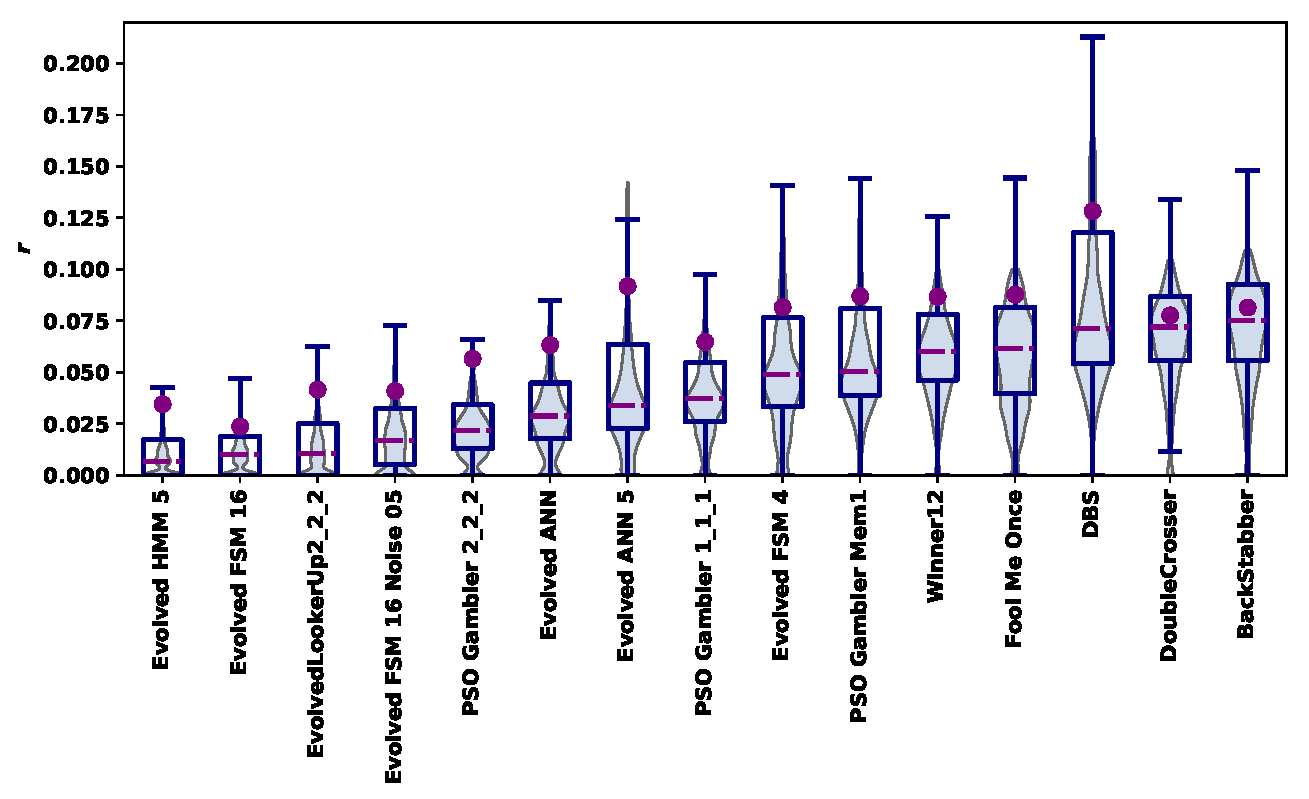
\includegraphics[width=\textwidth]{../images/r_distribution_standard.pdf}
        \caption{$r$ distributions of top 15 strategies in standard tournaments.}\label{fig:std_results}
    \end{subfigure}
    \hfill
    \begin{subfigure}{0.485\textwidth}
        \centering
        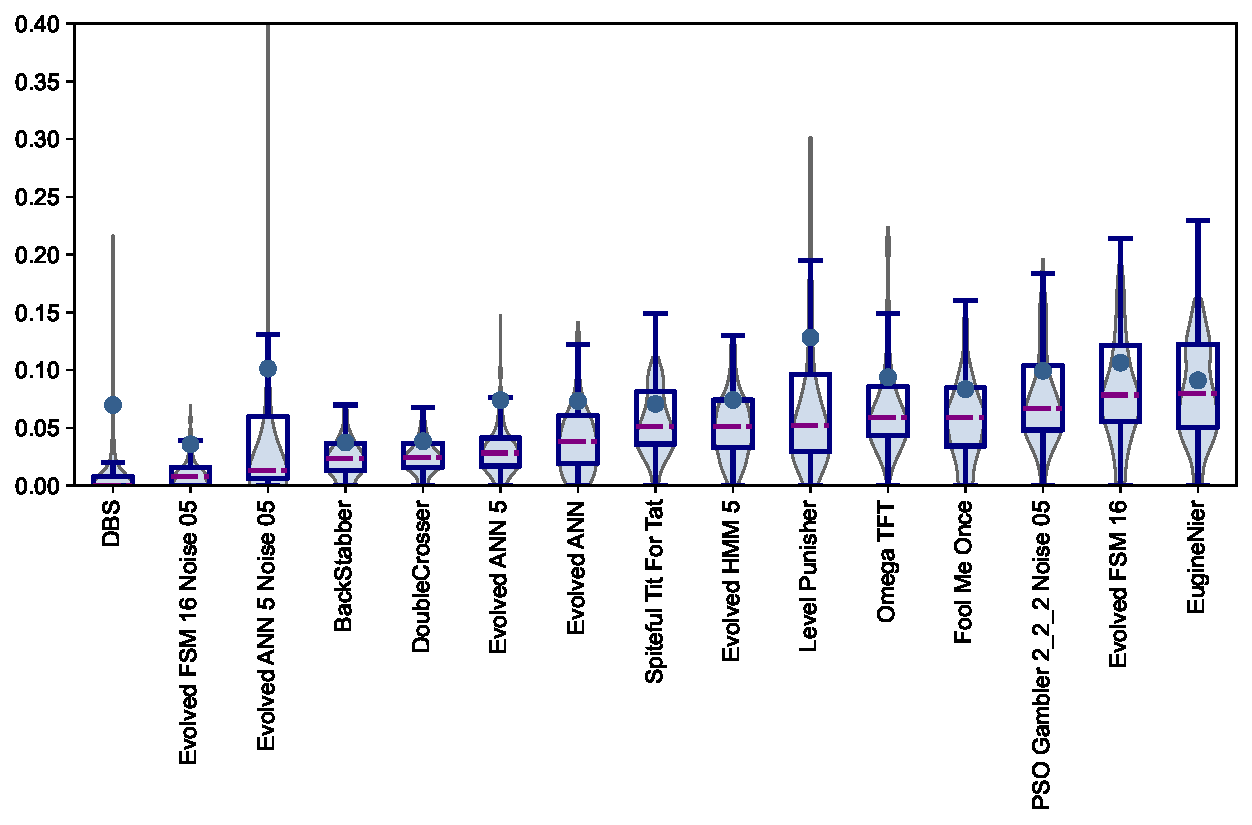
\includegraphics[width=\textwidth]{../images/r_distribution_noise_subset.pdf}
        \caption{$r$ distributions of top 15 strategies in noisy tournaments with \(p_n < 0.1\).}\label{fig:noise_subset_results}
    \end{subfigure}
    \vskip\baselineskip
    \begin{subfigure}{0.485\textwidth}
        \centering
        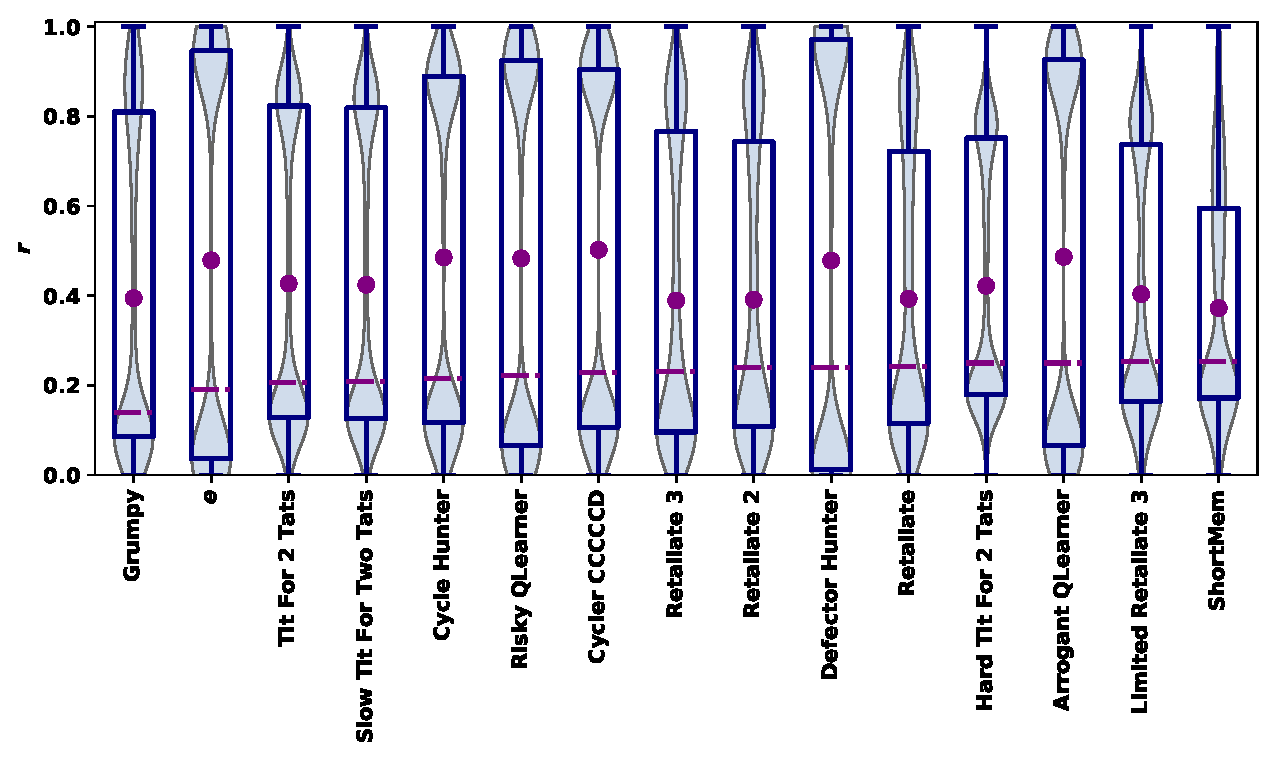
\includegraphics[width=\textwidth]{../images/r_distribution_noise.pdf}
        \caption{$r$ distributions of top 15 strategies in noisy tournaments.}\label{fig:noise_results}
    \end{subfigure}
    \quad
    \begin{subfigure}{0.485\textwidth}
        \centering
        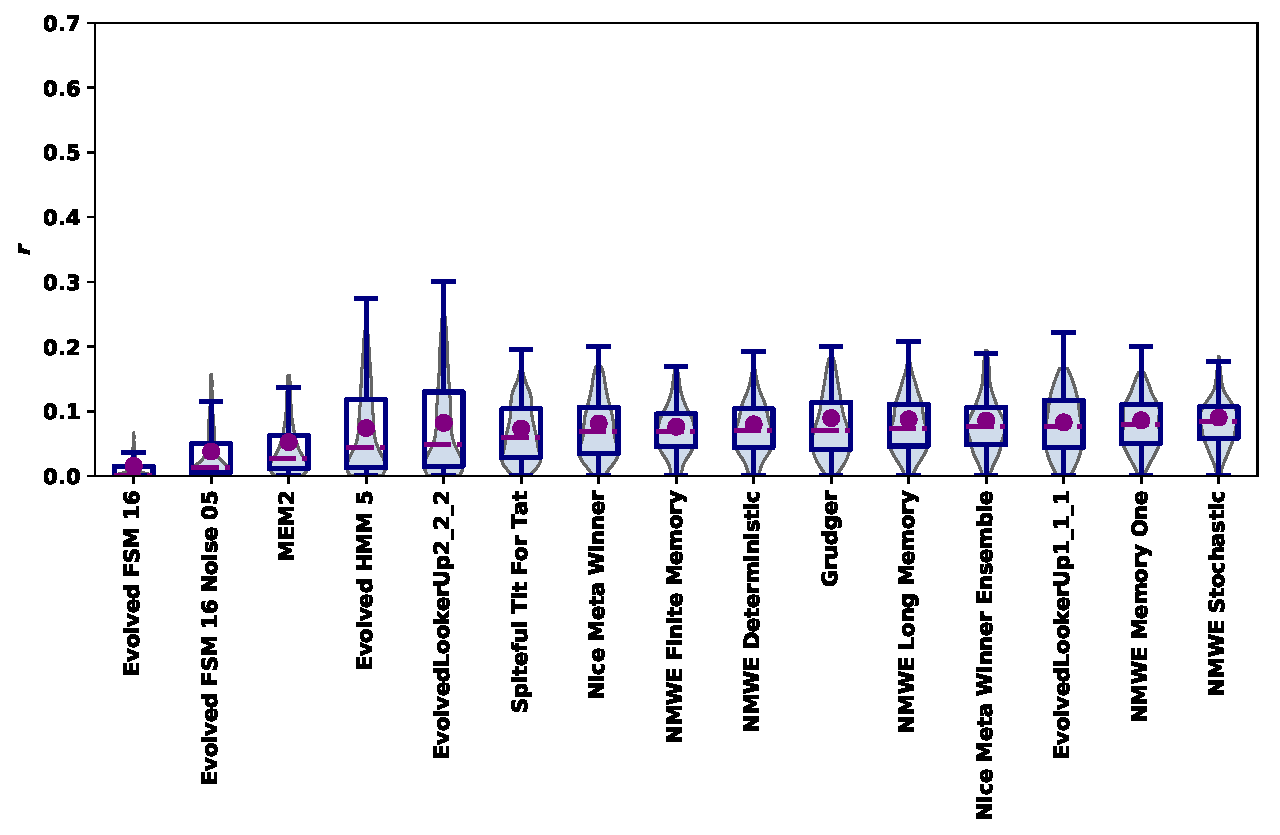
\includegraphics[width=\textwidth]{../images/r_distribution_probend_subset.pdf}
        \caption{\(r\) distributions of top 15 strategies in 1139 probabilistic ending
        tournaments with \(p_e < 0.1\).}
        \label{fig:probend_subset_results}
    \end{subfigure}
    \vskip\baselineskip
    \begin{subfigure}{0.485\textwidth}
        \centering
        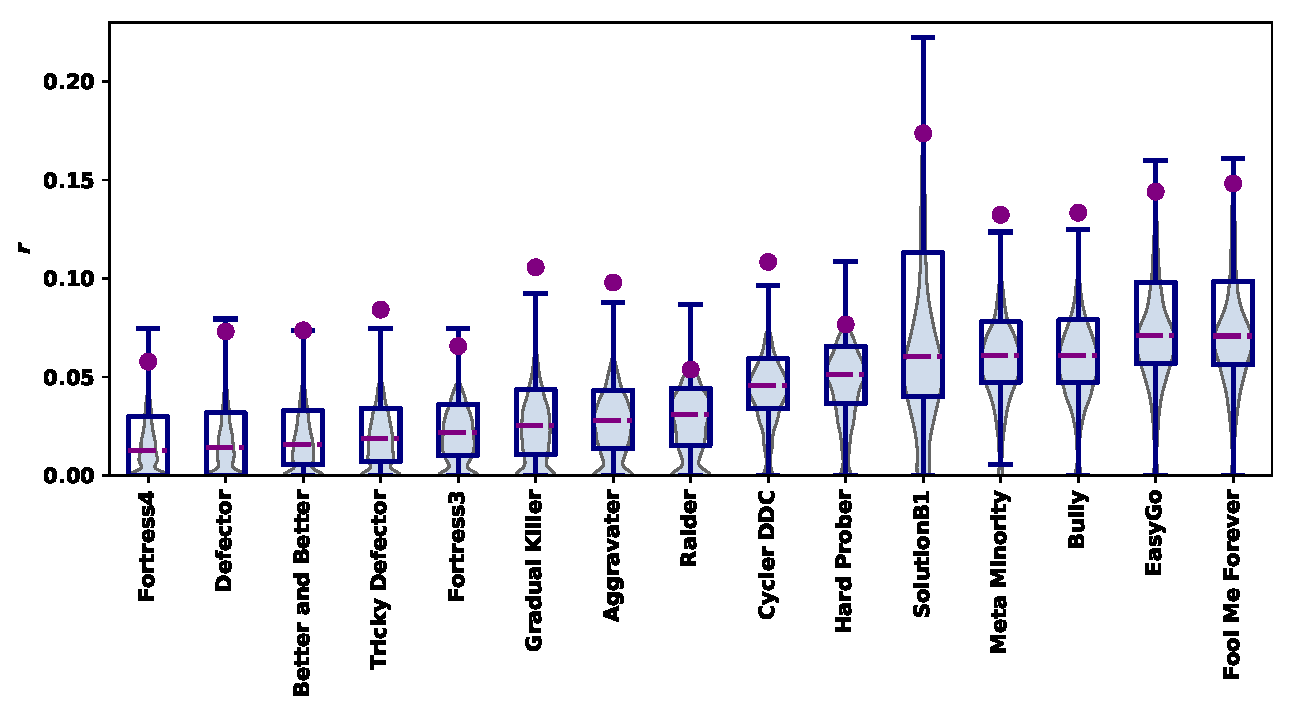
\includegraphics[width=\textwidth]{../images/r_distribution_probend.pdf}
        \caption{$r$ distributions of top 15 strategies in probabilistic ending tournaments.}\label{fig:probend_results}
    \end{subfigure}
    \quad
    \begin{subfigure}{0.485\textwidth}
        \centering
        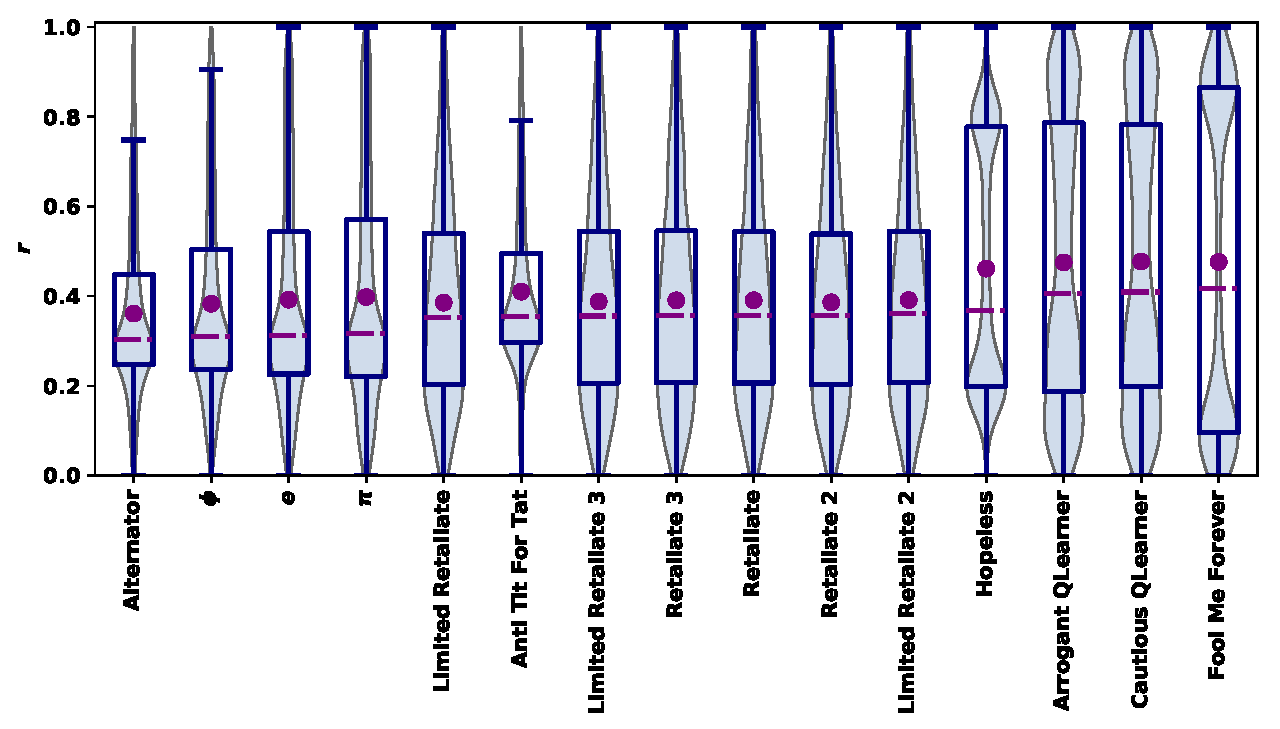
\includegraphics[width=\textwidth]{../images/r_distribution_probend_noise.pdf}
        \caption{$r$ distributions of top 15 strategies in noisy probabilistic ending tournaments.}
        \label{fig:probend_noise_results}
    \end{subfigure}
    \caption{\(r\) distributions of the top 15 strategies in different
    environments. A lower value of \(\bar{r}\) corresponds to a more successful
    performance. A strategy's \(r\) distribution skewed towards zero indicates
    that the strategy ranked highly in most tournaments it participated in. Most
    distributions are skewed towards zero except the distributions with
    unrestricted noise, supporting the conclusions from
    Table~\ref{table:top_performances}.}\label{fig:r_distributions}
\end{figure*}

In standard tournaments 10 out of the 15 top strategies were introduced
in~\cite{Harper2017}. These are strategies based on finite state automata (FSM),
hidden Markov models (HMM), artificial neural networks (ANN), lookup tables
(LookerUp) and stochastic lookup tables (Gambler) that have been trained using
reinforcement learning algorithms (evolutionary and particle swarm algorithms).
They have been trained to perform well against a subset of the strategies
in APL in a standard tournament, thus their performance in the
specific setting was anticipated although still noteworthy given the random
sampling of tournament participants. DoubleCrosser, BackStabber and Fool Me Once, are
strategies not from the literature but from the APL. DoubleCrosser is an extension
of BackStabber and both strategies make use of the number of turns because they are
set to defect on the last two rounds. It should be noted that these
strategies can be characterised as ``cheaters'' because the source code of the strategies
allows them to know the number of turns in a match (unless the match has a probabilistic ending). These strategies were expected to not perform as well in
tournaments where the number of turns is not specified. Finally, Winner
12~\cite{mathieu2017} and DBS~\cite{Au2006} are both from the literature.
DBS is a strategy specifically designed for noisy environments, however, it ranks
highly in standard tournaments as well. Similarly the fourth ranked player,
Evolved FSM 16 Noise 05, was
trained for noisy tournaments yet performs well in standard tournaments.
Figure~\ref{fig:std_results} shows that these strategies typically perform
well in any standard tournament in which they participate.

In the case of noisy tournaments with smaller noise \(p_n < 0.1\) the top
performing strategies
include strategies specifically designed for noisy tournaments. These are DBS,
Evolved FSM 16 Noise 05, Evolved ANN 5 Noise 05, PSO Gambler 2 2 2 Noise 05 and
Omega Tit For Tat~\cite{kendall2007iterated}. Omega TFT, a strategy designed
to break the deadlocking cycles of \(CD\) and \(DC\) that TFT can fall into in noisy
environments, places 10th. The rest of the top ranks are
occupied by strategies which performed well in standard tournaments and
deterministic strategies such as Spiteful Tit For Tat~\cite{prison}, Level
Punisher~\cite{Eckhart2015}, Eugine Nier~\cite{lesswrong}.

In contrast, the performance of the top ranked strategies in noisy environments
when \(p_n\in [0, 1]\) is bimodal. The top strategies include strategies which
decide their actions based on the cooperation to defection ratio, such as
ShortMem~\cite{Andre2013}, Grumpy~\cite{axelrodproject} and
e~\cite{axelrodproject}, and the Retaliate strategies which are designed to
defect if the opponent has tricked them more often than a given percentage of the times that
they have done the same. The bimodality of the \(r\) distributions is explained
by Figure~\ref{fig:effect_of_noise} which demonstrates that the top 6 strategies
were highly ranked due to the their performance in tournaments with \(p_n>0.5\),
and that in tournaments with \(p_n<0.5\) they
performed poorly. At a noisy level of \(0.5\) or greater, mostly cooperative strategies
become mostly defectors and vice versa.

\begin{figure}[!htbp]
    \centering
    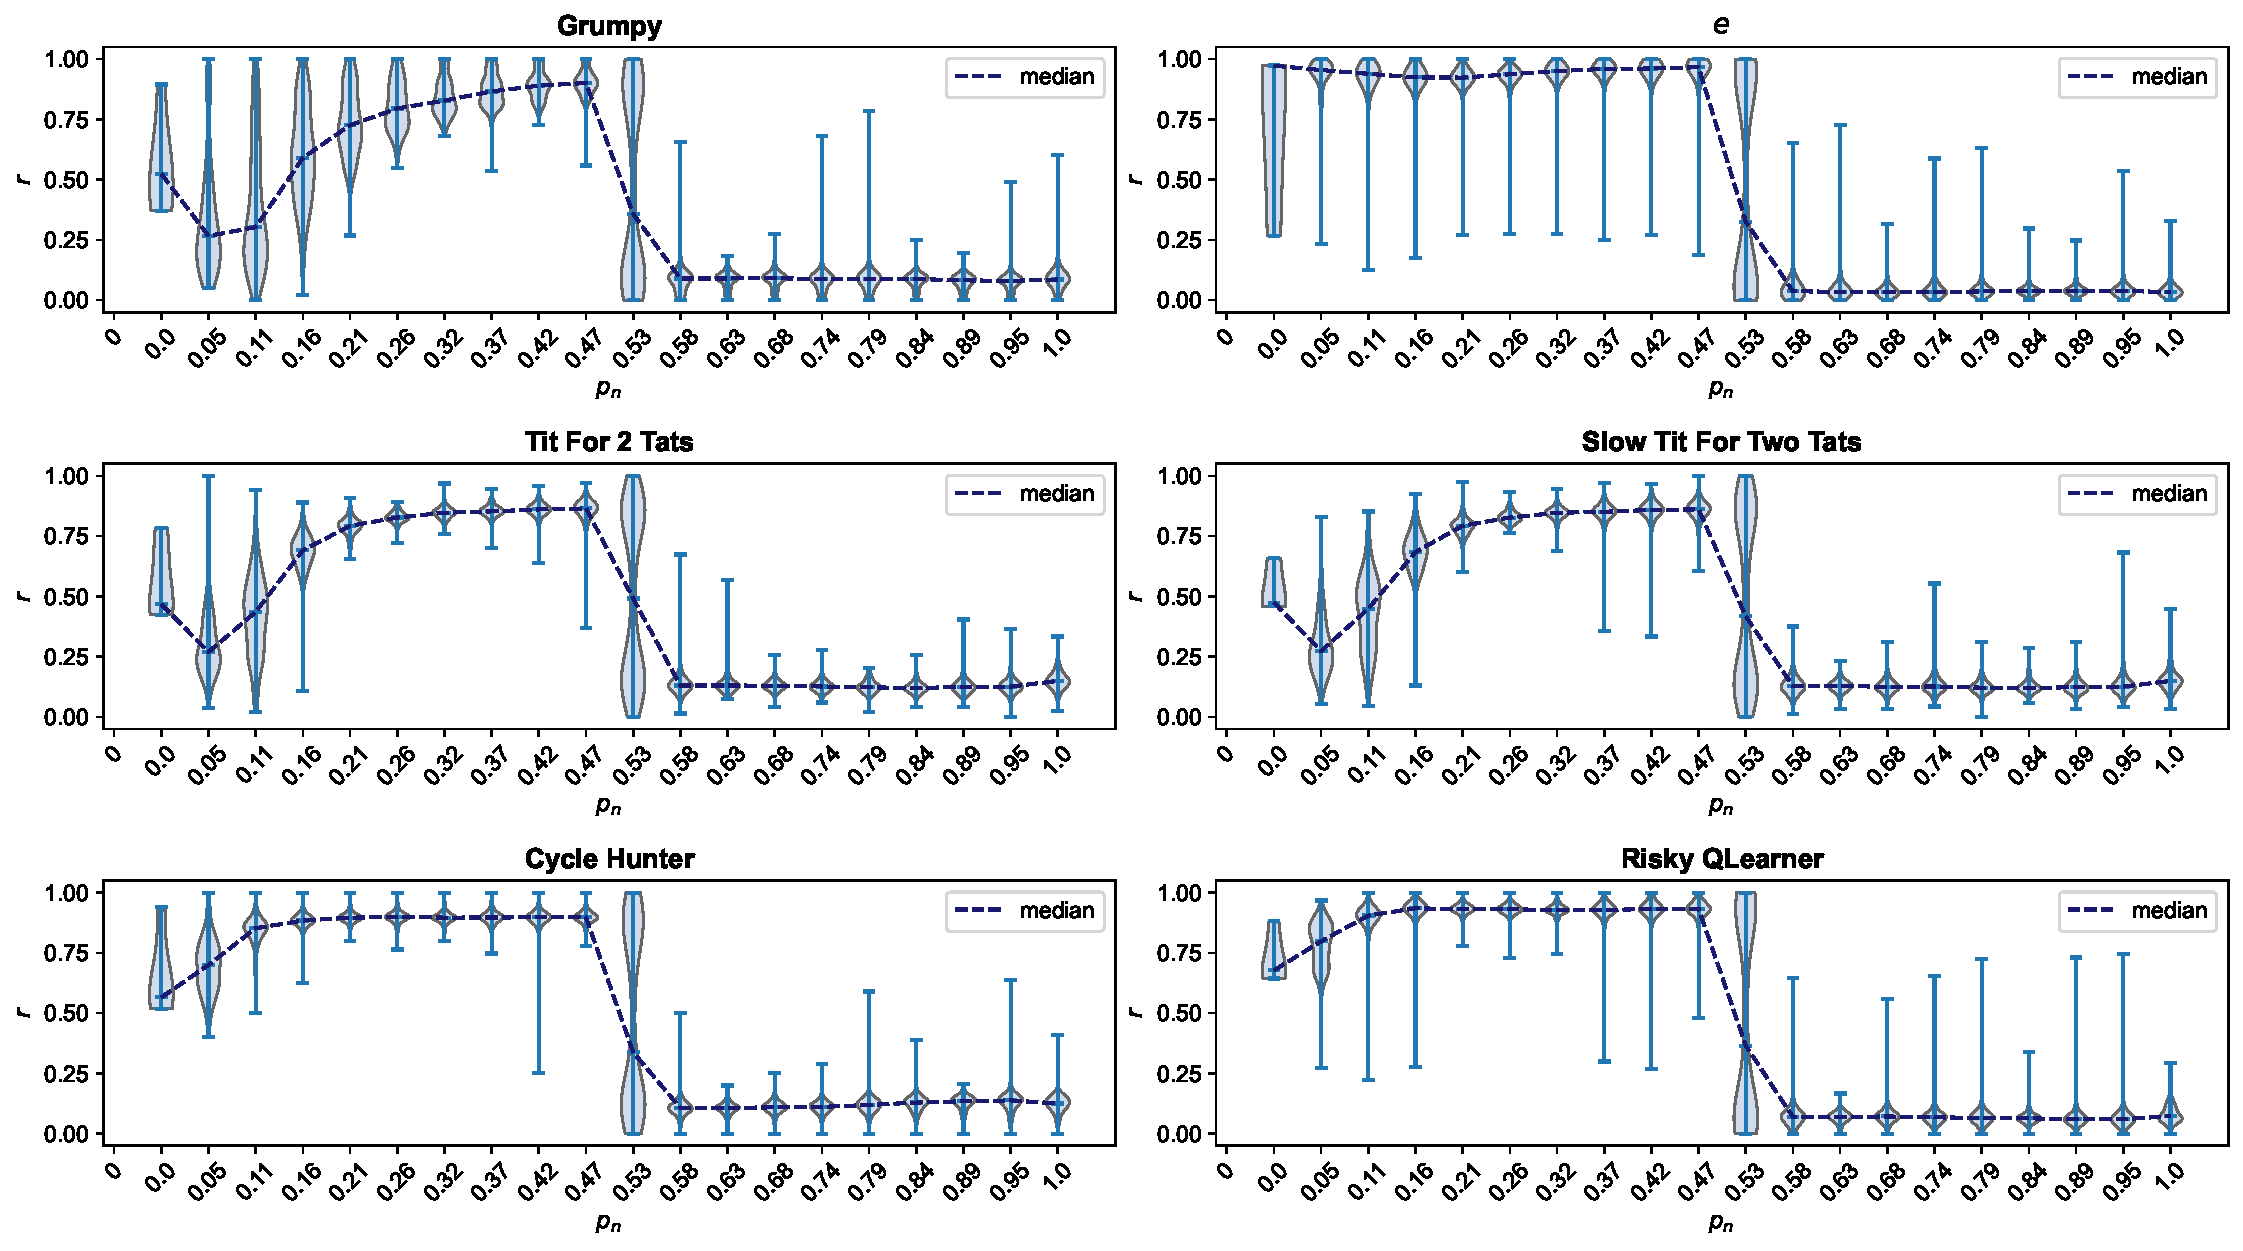
\includegraphics[width=.92\textwidth]{../images/noise_effect.pdf}
    \caption{Normalised rank \(r\) distributions for top 6 strategies in noisy tournaments over
    the probability of noisy ($p_n$).}
    \label{fig:effect_of_noise}
\end{figure}

The most effective strategies in probabilistic ending
tournaments with \(p_e< 0.1\) are a series of ensemble Meta strategies, trained strategies
which performed well
in standard tournaments, and Grudger~\cite{axelrodproject} and Spiteful Tit for
Tat~\cite{prison}. The Meta strategies~\cite{axelrodproject} utilize a team of
strategies and aggregate the potential actions of the team members into a single action
in various ways. Figure~\ref{fig:probend_subset_results} indicates that these strategies
performed well in any probabilistic ending tournament.

In probabilistic ending tournaments with \(p_e \in [0, 1]\) the top ranks are
mostly occupied by defecting strategies such as Better and Better, Gradual
Killer, Hard Prober (all from~\cite{axelrodproject}), Bully (Reverse Tit For
Tat)~\cite{Nachbar1992} and Defector, and a series of strategies based on finite
state automata introduced by Daniel Ashlock and Wendy Ashlock: Fortress 3,
Fortress 4 (both introduced in~\cite{Ashlock2006}), Raider~\cite{Ashlock2014}
and Solution B1~\cite{Ashlock2014}. The success of defecting strategies in
probabilistic ending tournaments is due to larger values of
\(p_e\) which lead to shorter matches (the expected number of rounds is \(1 / p_e\)), so the
impact of the PD being iterated is subdued. This is captured by the Folk
Theorem~\cite{Fudenberg2009} as defecting strategies do better when the likelihood
of the game ending in the next turn increases.
This is demonstrated by Figure~\ref{fig:effect_of_probend}, which gives the
distributions of \(r\) for the top 6 strategies in probabilistic ending tournaments
over \(p_e\).

\begin{figure}[!htbp]
    \centering
    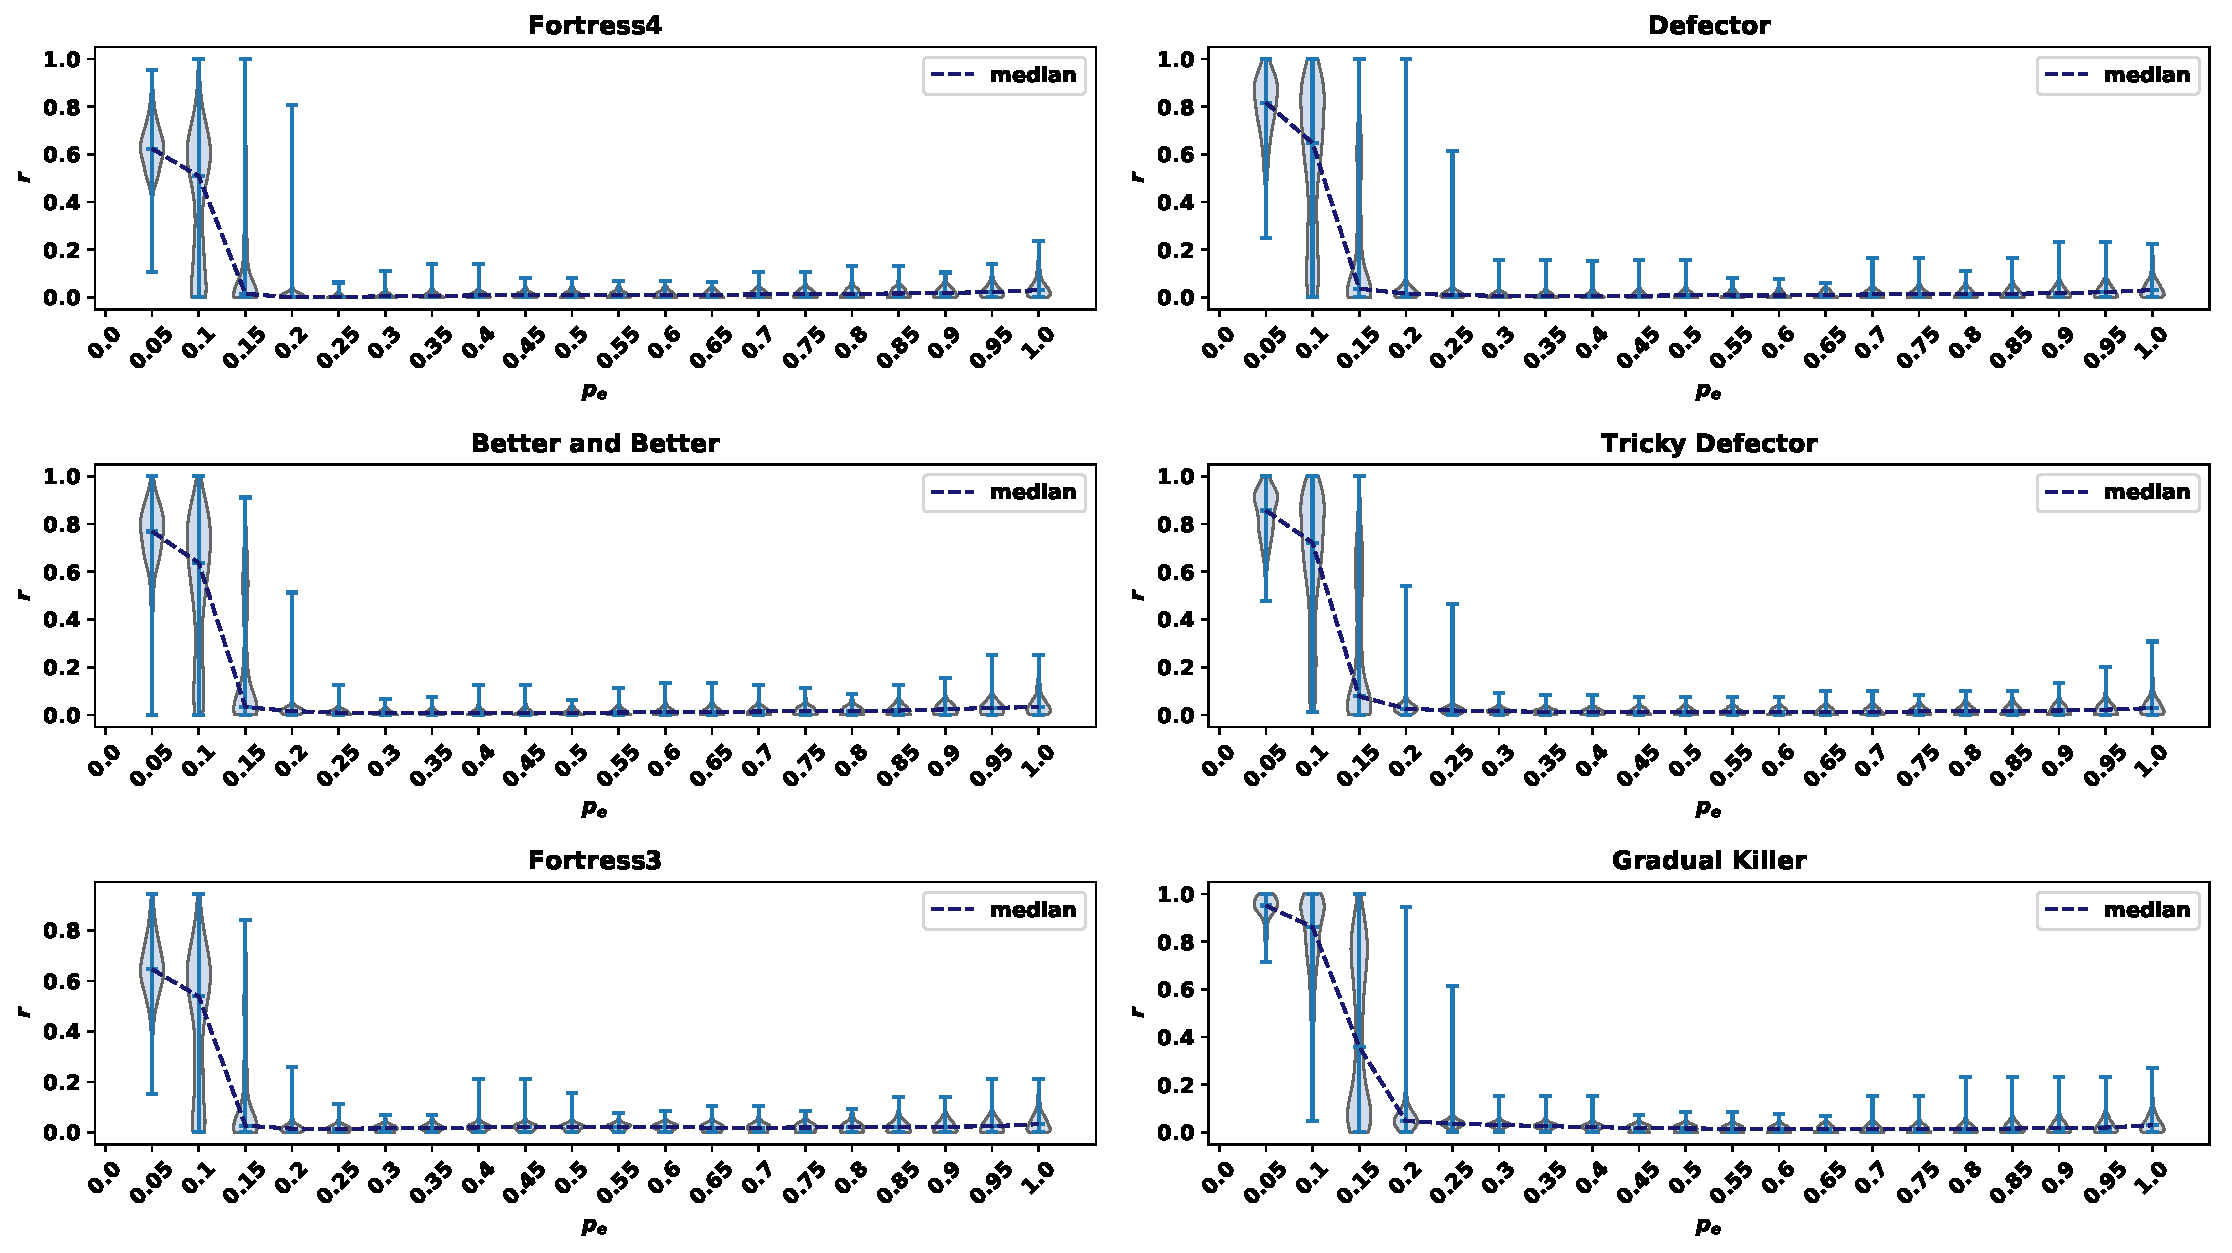
\includegraphics[width=.92\textwidth]{../images/folk_theorem.pdf}
    \caption{Normalised rank \(r\) distributions for top 6 strategies in probabilistic ending tournaments
    over $p_e$. The 6 strategies start of with a high median rank,
    however, their ranked decreased as the the probability of the game ending
    increased and at the point of \(p_e = 0.1\).}
    \label{fig:effect_of_probend}
\end{figure}

The top performances in tournaments with both noise and a probabilistic ending
have the largest median values compared to the top rank strategies of the other
tournament types. The \(\bar{r}\) for the top strategy is approximately at 0.3,
indicating that the most successful strategy can on average just place in the
top 30\% of the competition.

On the whole, the analysis has shown that:

\begin{itemize}
    \item In standard tournaments the dominating strategies were
    strategies that had been trained using reinforcement learning techniques.
    \item In noisy environments where the noise probability strictly less than
    0.1 was considered, the successful strategies were strategies specifically
    designed or trained for noisy environments.
    \item In probabilistic ending tournaments most of the highly ranked
    strategies were defecting strategies and trained finite state automata, all
    by the authors of~\cite{Ashlock2006, Ashlock2014}. These strategies ranked
    high due to their performance in tournaments where the probability of the
    game ending after each turn was bigger than 0.1.
    \item In probabilistic tournaments with \(p_e\) less than 0.1 the highly
    ranked strategies were strategies based on the behaviour of others.
    \item From the collection of strategies considered here,  no strategy can be
    consistently successful in noisy environments, except if the value of noise
    is constrained to less than a 0.1.
\end{itemize}

\section{The effect of strategy features on performance}

The correlation coefficients between the strategies' features and the median
score and the median normalised rank for the full dataset of tournaments are
given by Table~\ref{table:correlations}. The correlation coefficients between
all features have been calculated and a graphical representation can be found in
the Section~\ref{app:correlations}.

\newcolumntype{g}{>{\columncolor{Gray}}c}
\begin{table}[!htbp]
    \begin{center}
    \resizebox{.9\textwidth}{!}{
        \begin{tabular}{lggccggccggg}
    \toprule
    &  \multicolumn{2}{g}{Standard} & \multicolumn{2}{c}{Noisy} & \multicolumn{2}{g}{Probabilistic ending} &  \multicolumn{2}{c}{Noisy probabilistic ending} \\
\midrule
{} &  $r$ &  median score &  $r$ &  median score &  $r$ &  median score &  $r$ &  median score \\
\midrule
$CC$ to $C$ rate & -0.501 & 0.501 & 0.413 & -0.504 & 0.408 & -0.323 & 0.260 & 0.023 \\
$CD$ to $C$ rate & 0.226 & -0.199 & 0.457 & -0.331 & 0.320 & -0.017 & 0.205 & -0.220 \\
$DC$ to $C$ rate & 0.127 & -0.100 & 0.509 & -0.504 & -0.018 & 0.033 & 0.341 & -0.016 \\
$DD$ to $C$ rate & 0.412 & -0.396 & 0.533 & -0.436 & -0.103 & 0.176 & 0.378 & -0.263 \\
$C_r$ & -0.323 & 0.383 & 0.711 & -0.678 & 0.714 & -0.832 & 0.579 & -0.136 \\
$C_{max}$ & 0.000& 0.050 & 0.000& 0.023 & -0.000& 0.046 & 0.000& -0.004 \\
$C_{min}$ & 0.000& 0.085 & -0.000& -0.017 & -0.000& 0.007 & -0.000& 0.041 \\
$C_{median}$ & 0.000& 0.209 & -0.000& 0.240 & 0.000& 0.187 & 0.000& 0.673 \\
$C_{mean}$ & 0.000& 0.229 & -0.000& 0.271 & 0.000& 0.200 & -0.000& 0.690 \\
$C_r$ / $C_{max}$  & -0.323 & 0.381 & 0.616 & -0.551 & 0.715 & -0.833 & 0.536 & -0.117 \\
$C_{min}$ / $C_r$ & 0.109 & -0.080 & -0.358 & 0.250 & -0.134 & 0.151 & -0.368 & 0.113 \\
$C_r$ / $C_{median}$ & -0.330 & 0.353 & 0.652 & -0.669 & 0.713 & -0.852 & 0.330 & -0.466 \\
$C_r$ / $C_{mean}$ & -0.331 & 0.357 & 0.731 & -0.740 & 0.721 & -0.861 & 0.650 & -0.621 \\
$N$ & -0.000& -0.009 & 0.000& 0.002 & 0.000& 0.003 & 0.000& 0.001 \\
$k$ & -0.000& -0.002 & 0.000& 0.002 & 0.000& 0.001 & 0.000& -0.008 \\
$n$ & -0.000& -0.125 & -0.000& -0.024 & - & - & - & - \\
$p_n$ & - & - & 0.000& 0.207 & - & - & 0.000& -0.650 \\
$p_e$ & - & - & - & - & 0.000& 0.165 & 0.000& -0.058 \\
Make use of game & -0.003 & -0.022 & 0.025 & -0.082 & -0.053 & -0.108 & 0.013 & -0.016 \\
Make use of length & -0.158 & 0.124 & 0.005 & -0.123 & -0.025 & -0.090 & 0.014 & -0.016 \\
SSE & 0.473 & -0.452 & 0.463 & -0.337 & -0.157 & 0.224 & 0.305 & -0.259 \\
stochastic & 0.006 & -0.024 & 0.022 & -0.026 & 0.002 & -0.130 & 0.021 & -0.013 \\
memory usage & -0.098 & 0.108 & -0.009 & -0.017 & - & - & - & - \\
\bottomrule
\end{tabular}
    }
\end{center}
\caption{Correlations between the strategies' features
and the normalised rank and the median score.}\label{table:correlations}
\end{table}

In standard tournaments the features $CC$ to $C$, $C_r$, $C_r / C_{\text{max}}$
and the cooperating ratio compared to $C_{\text{median}}$ and $C_{\text{mean}}$
have a moderately negative effect on the normalised rank (smaller rank is
better), and a moderate positive on the median score. The SSE error and the $DD$
to $C$ rate have the opposite effects. Thus, in standard tournaments behaving
cooperatively corresponds to a more successful performance. Even though being
nice generally pays off that does not hold against defective strategies. Being
more cooperative after a mutual defection, that is not retaliating, is
associated to lesser overall success in terms of normalised rank.
Figure~\ref{fig:rates_of_winners_in_standard_tournaments} confirms that the
winners of standard tournaments always cooperate after a mutual cooperation and
almost always defect after a mutual defection.

\begin{figure}[!htbp]
    \centering
    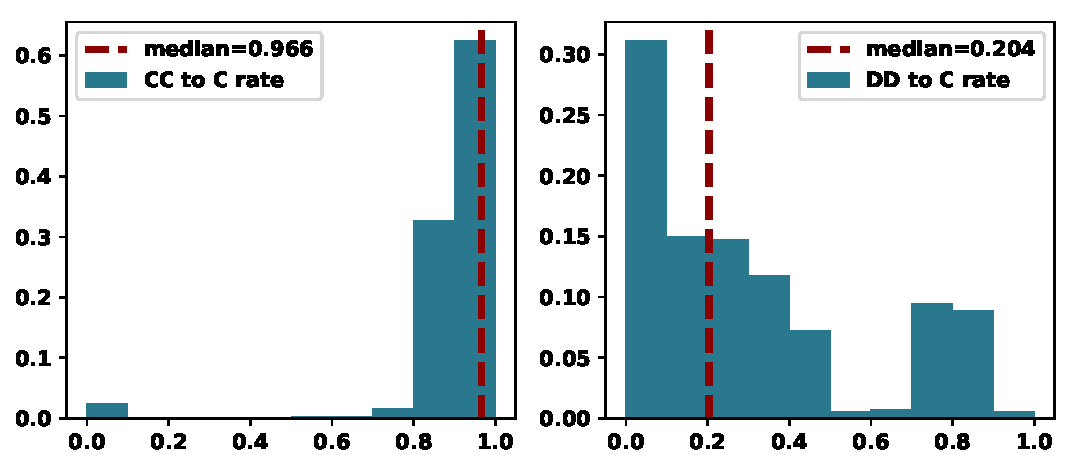
\includegraphics[width=.8\textwidth]{../images/rates_of_winners_in_standard_tournaments.pdf}
    \caption{Distributions of $CC$ to $C$ and $DD$ to $C$ for the winners in
    standard tournaments.}\label{fig:rates_of_winners_in_standard_tournaments}
\end{figure}

Compared to standard tournaments, in both noisy and in probabilistic ending
tournaments the higher the rates of cooperation the lower a strategy's success
and median score. A strategy would want to cooperate less than both the mean and
median cooperator in such settings. In probabilistic ending tournaments the
correlation coefficients have larger values, indicating a stronger effect. Thus
a strategy will be punished more by its cooperative behaviour in probabilistic
ending environments, supporting the results of the previous subsection as well.
The distributions of the $C_r$ of the winners in both tournaments are given by
Figure~\ref{fig:c_r_distributions}. It confirms that the winners in noisy
tournaments cooperated less than 35\% of the time and in probabilistic ending
tournaments less than 10\%. In noisy probabilistic ending tournaments and over
all the tournaments' results, the only features that had a moderate effect are
$C_r/C_{\text{mean}}, C_r/C_{\text{max}}$ and $C_r$. In such environments
cooperative behaviour appears to be punished less than in noisy and
probabilistic ending tournaments.


\begin{figure}[!htbp]
    \centering
    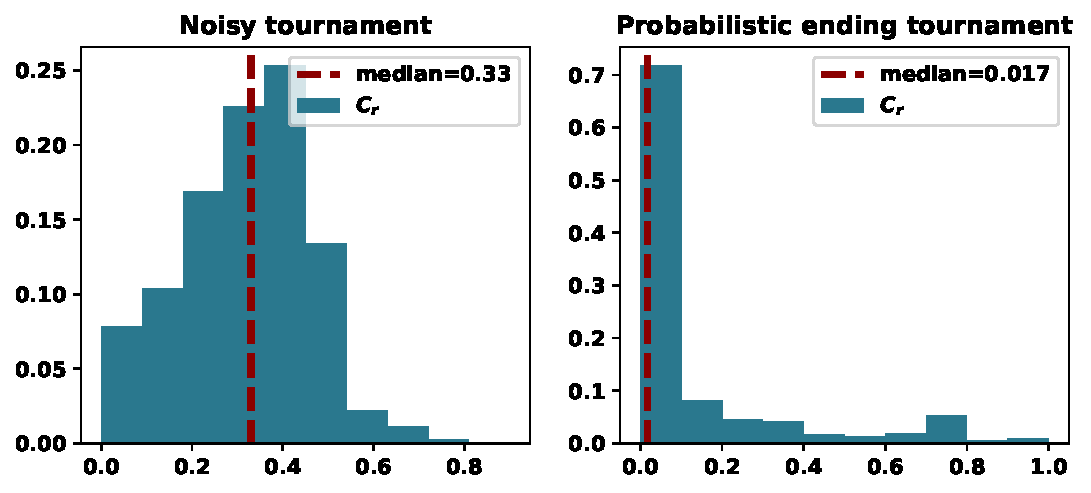
\includegraphics[width=.8\textwidth]{../images/c_r_winners_tournaments.pdf}
    \caption{$C_r$ distributions of the winners in noisy and in probabilistic
    ending tournaments.}\label{fig:c_r_distributions}
\end{figure}

A multivariate linear regression has been fitted to model the relationship between
the features and the normalised rank. Based on the graphical representation of
the correlation matrices given in Section~\ref{app:correlations} several of the
features are highly correlated and have been removed
before fitting the linear regression model. The features included are given
by Table~\ref{table:linear_regression} alongside their corresponding \(p\) values
in the distinct tournaments and their regression coefficients.

\newcolumntype{g}{>{\columncolor{Gray}}c}
\begin{table}[h]
    \begin{center}
\resizebox{\textwidth}{!}{
    \begin{tabular}{lggccggccgg}
\toprule
& \multicolumn{2}{g}{Standard} & \multicolumn{2}{c}{Noisy} & \multicolumn{2}{g}{Probabilistic ending} & \multicolumn{2}{c}{Noisy probabilistic ending} \\
\midrule
& \multicolumn{2}{g}{\(R\) adjusted: 0.541} & \multicolumn{2}{c}{\(R\) adjusted: 0.588} & \multicolumn{2}{g}{\(R\) adjusted: 0.587} & \multicolumn{2}{c}{\(R\) adjusted: 0.471} \\
{} &  Coefficient &  \(p\)-value &  Coefficient &  \(p\)-value &  Coefficient &  \(p\)-value &  Coefficient &  \(p\)-value \\
\midrule
constant           &  0.695 &  0.000 &  0.443 &    0.0 & -0.057 &  0.018 &  0.004 &  0.031 \\
$CC$ to $C$ rate   & -0.042 &  0.000 &  0.150 &    0.0 &  0.017 &  0.000 &  0.197 &  0.000 \\
$CD$ to $C$ rate   &  0.297 &  0.000 & -0.034 &    0.0 &  0.182 &  0.000 &  0.022 &  0.000 \\
$DC$ to $C$ rate   &  0.198 &  0.000 &  0.064 &    0.0 & -0.030 &  0.000 &  0.090 &  0.000 \\
SSE                &  0.258 &  0.000 &  0.237 &    0.0 & -0.041 &  0.000 &  0.144 &  0.000 \\
$C_{max}$          & -0.068 &  0.000 &      - &      - & -0.021 &  0.403 & -0.090 &  0.000 \\
$C_{min}$          & -0.161 &  0.000 &  1.068 &    0.0 & -0.170 &  0.000 &      - &      - \\
$C_{mean}$         &  0.117 &  0.000 & -0.722 &    0.0 & -0.024 &  0.000 & -0.112 &  0.000 \\
$C_{min}$ / $C_r$  &  0.057 &  0.000 & -0.544 &    0.0 &  0.125 &  0.000 &      - &      - \\
$C_r$ / $C_{mean}$ & -0.468 &  0.000 &  0.272 &    0.0 &  0.525 &  0.000 &  0.403 &  0.000 \\
$k$                &  0.000 &  0.325 &  0.000 &    0.1 &  0.000 &  0.002 &  0.001 &  0.000 \\
$n$                &  0.000 &  0.000 &      - &      - &      - &      - &      - &      - \\
memory usage       & -0.010 &  0.000 &  0.002 &    0.0 &      - &      - &      - &      - \\
$p_n$              &      - &      - & -0.039 &    0.0 &      - &      - &      - &      - \\
$p_e$              &      - &      - &      - &      - &  0.000 &  0.757 & -0.149 &  0.000 \\
\bottomrule
\end{tabular}}
    \end{center}
    \caption{Results of multivariate linear regressions with \(r\) as the dependent variable.
    \(R\) squared is reported for each model.}
    \label{table:linear_regression}
\end{table}

A multivariate linear regression has also be fitted on the median score. The
coefficients and \(p\) values of the features can be found in
Section~\ref{app:regression_median_score}. This approach leads to similar conclusions.

The feature \(C_{r} / C_{\text{mean}}\) has a statistically significant effect
across all models and a high regression coefficient. It has both a positive and
negative impact on the normalised rank depending on the environment. For
standard tournaments, Figure~\ref{fig:discussion_standard} gives the
distributions of several features for the winners of standard tournaments. The
\(C_{r} / C_{\text{mean}}\) distribution of the winner is also given in
Figure~\ref{fig:discussion_standard}. A value of \(C_r / C_{\text{mean}} = 1\)
implies that the cooperating ratio of the winner was the same as the mean
cooperating ratio of the tournament, and in standard tournaments, the median is
1. Therefore, an effective strategy in standard tournaments was the mean
cooperator of its respective tournament.

The distributions of SSE and \(CD\) to \(C\) rate for the winners of standard
tournaments are also given in Figure~\ref{fig:discussion_standard}. The SSE
distributions for the winners indicate that the strategy behaved in a ZD way in
several tournaments, however, not constantly. The winners participated in
matches where they did not try to extortionate their opponents. Furthermore, the
\(CD\) to \(C\) distribution indicates that if a strategy were to defect against
the winners the winners would reciprocate on average with a probability of 0.5.

\begin{figure}[!htbp]
    \centering
        \centering
        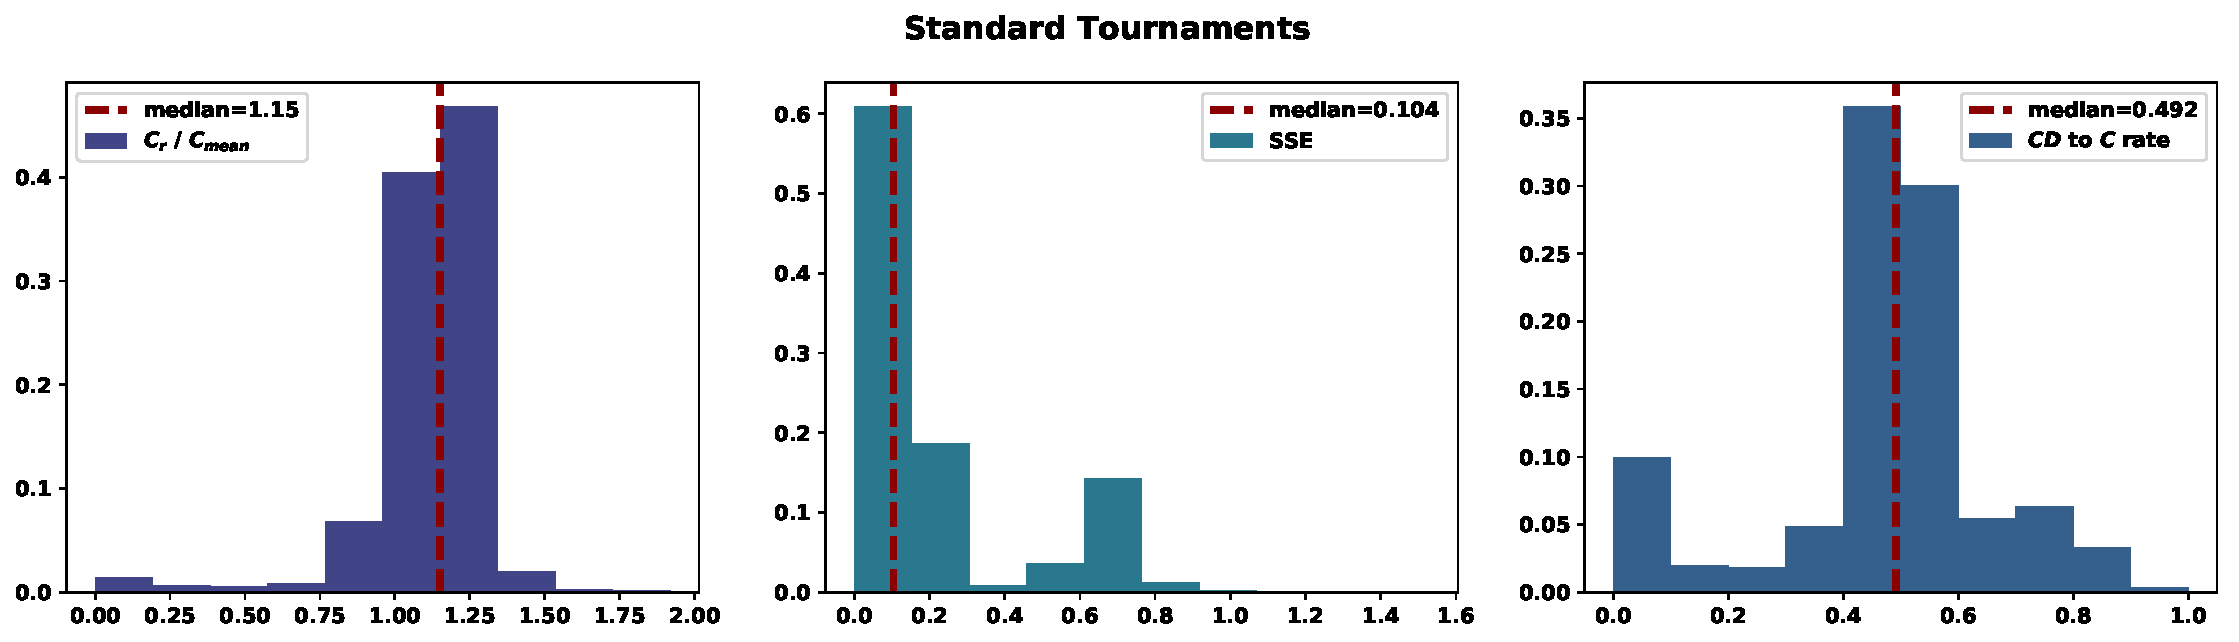
\includegraphics[width=\textwidth]{../images/standard_discussion.pdf}
        \caption{Distributions of \(C_r / C_{\text{mean}}\), SSE and \(CD\) to \(C\) ratio
        for the winners of standard tournaments. A
        value of \(C_r / C_{\text{mean}} = 1\) imply that the cooperating ratio of the
        winner was the same as the mean cooperating ratio of the tournament. An SSE distribution
        skewed towards 0 indicates a extortionate behaviour by the strategy.}
        \label{fig:discussion_standard}
\end{figure}

Similarly for the rest of the different tournaments types, and the entire data
set the distributions of \(C_r / C_{\text{mean}}\), SSE and \(CD\) to \(C\) ratio
are given by Figures~\ref{fig:discussion_noisy},~\ref{fig:discussion_probend},
\ref{fig:discussion_probend_noisy} and~\ref{fig:discussion_entire_data}.

Based on the \(C_r / C_{\text{mean}}\) distributions the successful strategies
have adapted differently to the mean cooperator depending on the tournament
type. In noisy tournaments where the median of the distribution is at 0.67, and
thereupon the winners cooperated 67\% of the time the mean cooperator did. In
tournaments with noise and a probabilistic ending the winners cooperated 60\%,
whereas in settings that the type of the tournament can vary between all the
types the winners cooperated 67\% of the time the mean cooperator did. Lastly,
in probabilistic ending tournaments above more defecting
strategies prevail (Section~\ref{section:top_performances}), and this result is
reflected here.

\begin{figure}[!htbp]
    \centering
        \centering
        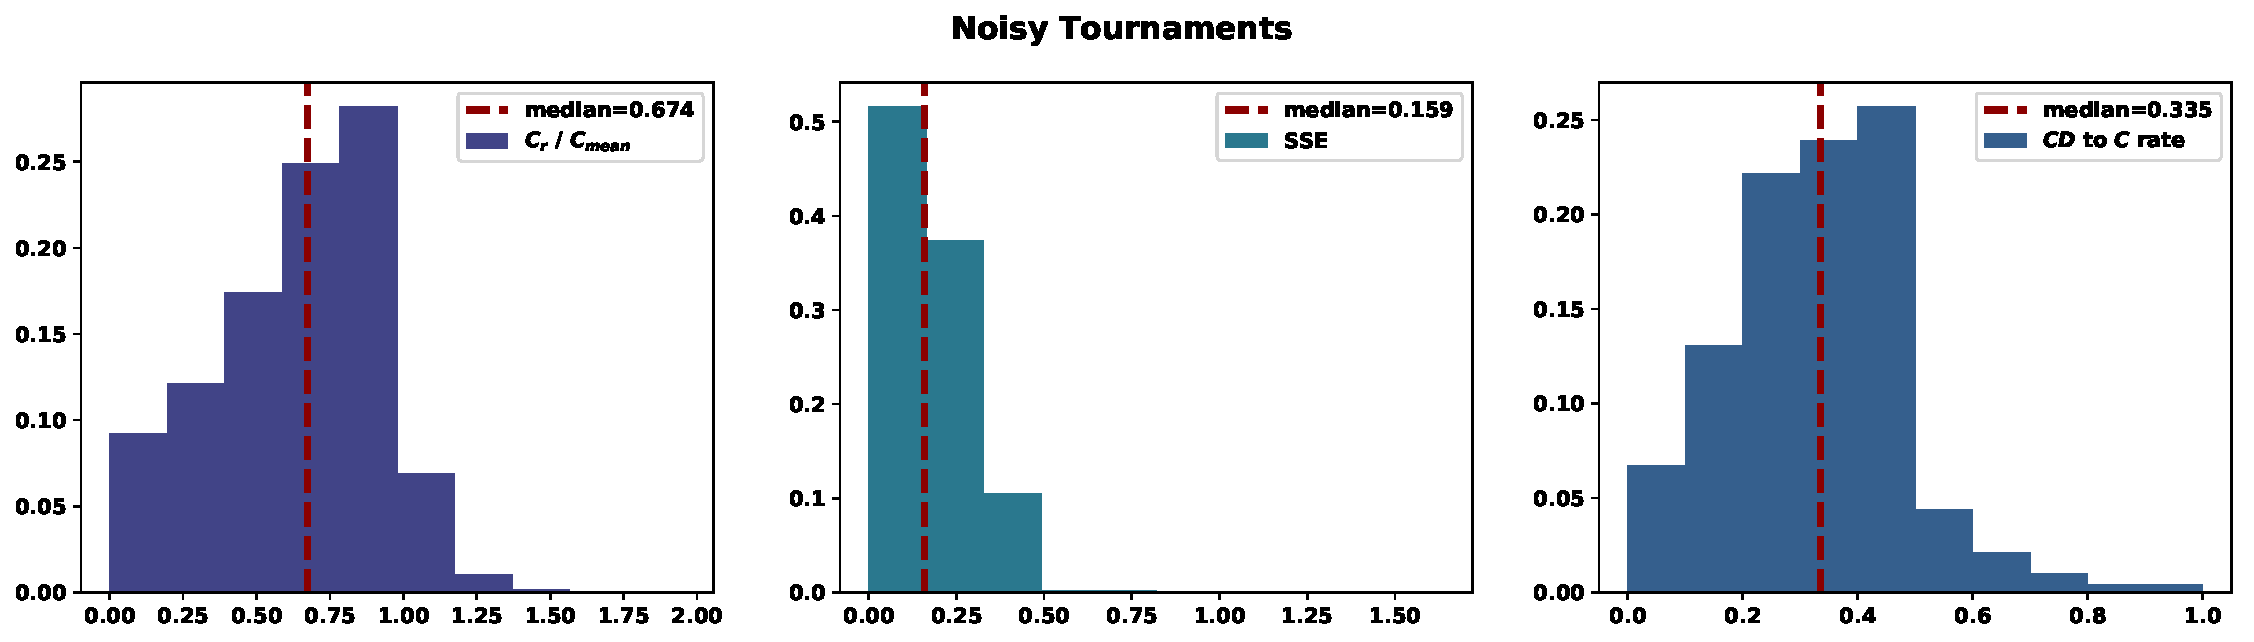
\includegraphics[width=\textwidth]{../images/noisy_discussion.pdf}
        \caption{Distributions of \(C_r / C_{\text{mean}}\), SSE and \(CD\) to \(C\) ratio
        for the winners of noisy tournaments.}
        \label{fig:discussion_noisy}
\end{figure}

The probability of noise has been observed to substantially affect optimal
behaviour.
Figure~\ref{fig:compared_to_mean_over_noise_probability} gives the ratio \(C_r /
C_{\text{mean}}\) for the winners in tournaments with noise, over the
probability of noise. From Figure~\ref{fig:noisy_discussion_over_noise} it is
clear that the cooperating only 67\% of the time the mean cooperator did is
optimal only when \(p_n \in [0.2, 0.4)\) and \(p_n \in [0.6, 0.7]\). In
environments with \(p_n < 0.1\) the winners want to be close to the mean
cooperator, similarly to standard tournaments, and as the probability of noise
is exceeding 0.5 (where the game is effectively inverted) strategies should
aim to be less and less cooperative.

Figure~\ref{fig:compared_to_mean_over_noise_probability} gives \(C_r /
C_{\text{mean}}\) for the winners over \(p_n\) in tournaments with noise and a
probabilistic ending. The optimal proportions of cooperations are different
now that the number of turns is not fixed, successful strategies
want to be more defecting that the mean cooperator, that only changes when
\(p_n\) approaches 0.5. Figure~\ref{fig:compared_to_mean_over_noise_probability}
demonstrates how the adjustments to \(C_r /C_{\text{mean}}\) change over the
noise in the to the environment, and thus supports how important adapting to
the environment is for a strategy to be successful.

\begin{figure}[!htbp]
    \centering
    \begin{subfigure}{0.485\textwidth}
        \centering
        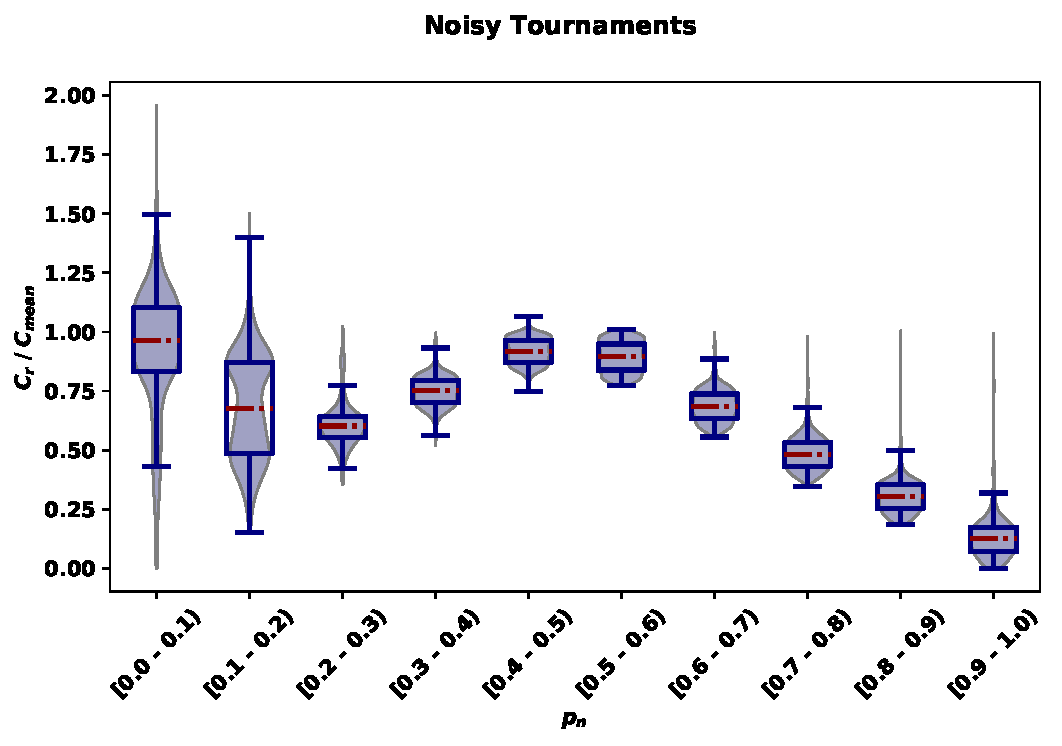
\includegraphics[width=\textwidth]{../images/noisy_discussion_over_noise.pdf}
        \caption{\(C_r / C_{\text{mean}}\) distribution for winners in noisy tournaments over
        \(p_n\).}\label{fig:noisy_discussion_over_noise}
    \end{subfigure}
    \hfill
    \begin{subfigure}{0.485\textwidth}
        \centering
        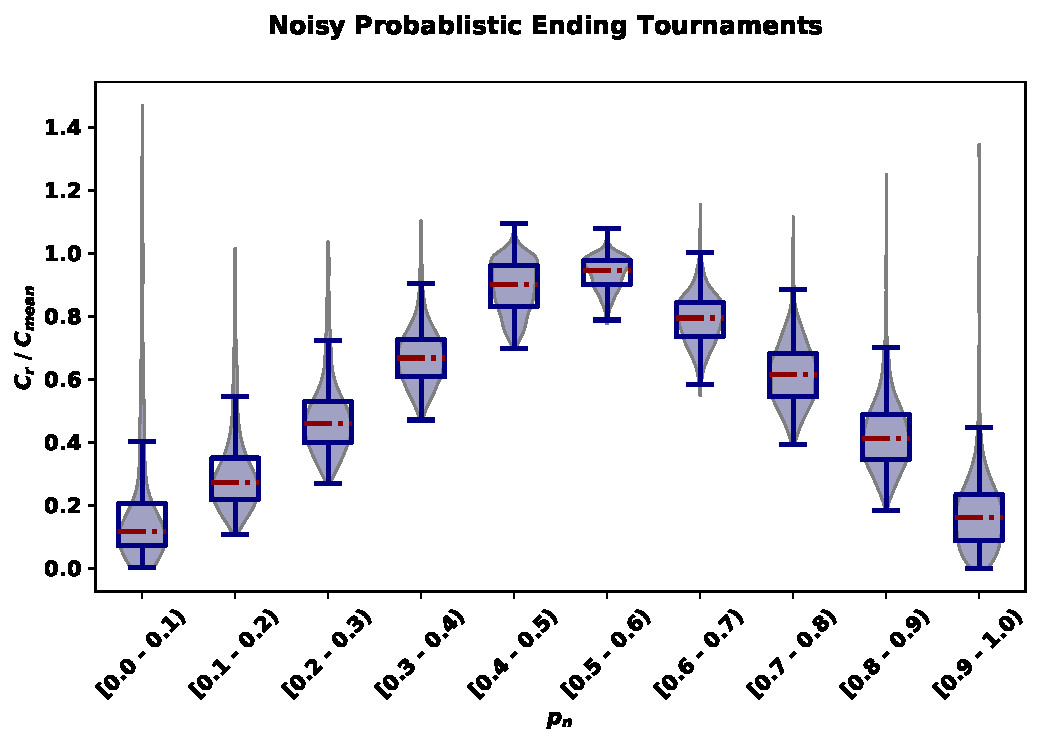
\includegraphics[width=\textwidth]{../images/noisy_probend_discussion_over_noise.pdf}
        \caption{\(C_r / C_{\text{mean}}\) distribution for winners in noisy probabilistic ending tournaments over
        \(p_n\).}\label{fig:noisy_probend_discussion_over_noise}
    \end{subfigure}
    \caption{\(C_r / C_{\text{mean}}\) distributions over intervals of \(p_n\).
    These distributions model the optimal proportion of cooperation
    compared to \(C_{\text{mean}}\) as a function of (\(p_n\)).}
    \label{fig:compared_to_mean_over_noise_probability}
\end{figure}

The distributions of the SSE across the tournament types suggest that successful
strategies exhibit some extortionate behaviour, but not constantly.
ZDs are a set of strategies that are often envious as they try to exploit their
opponents. The winners of the tournaments considered in this work are
envious, but not as much as many ZDs.

\begin{figure}[!htbp]
    \centering
        \centering
        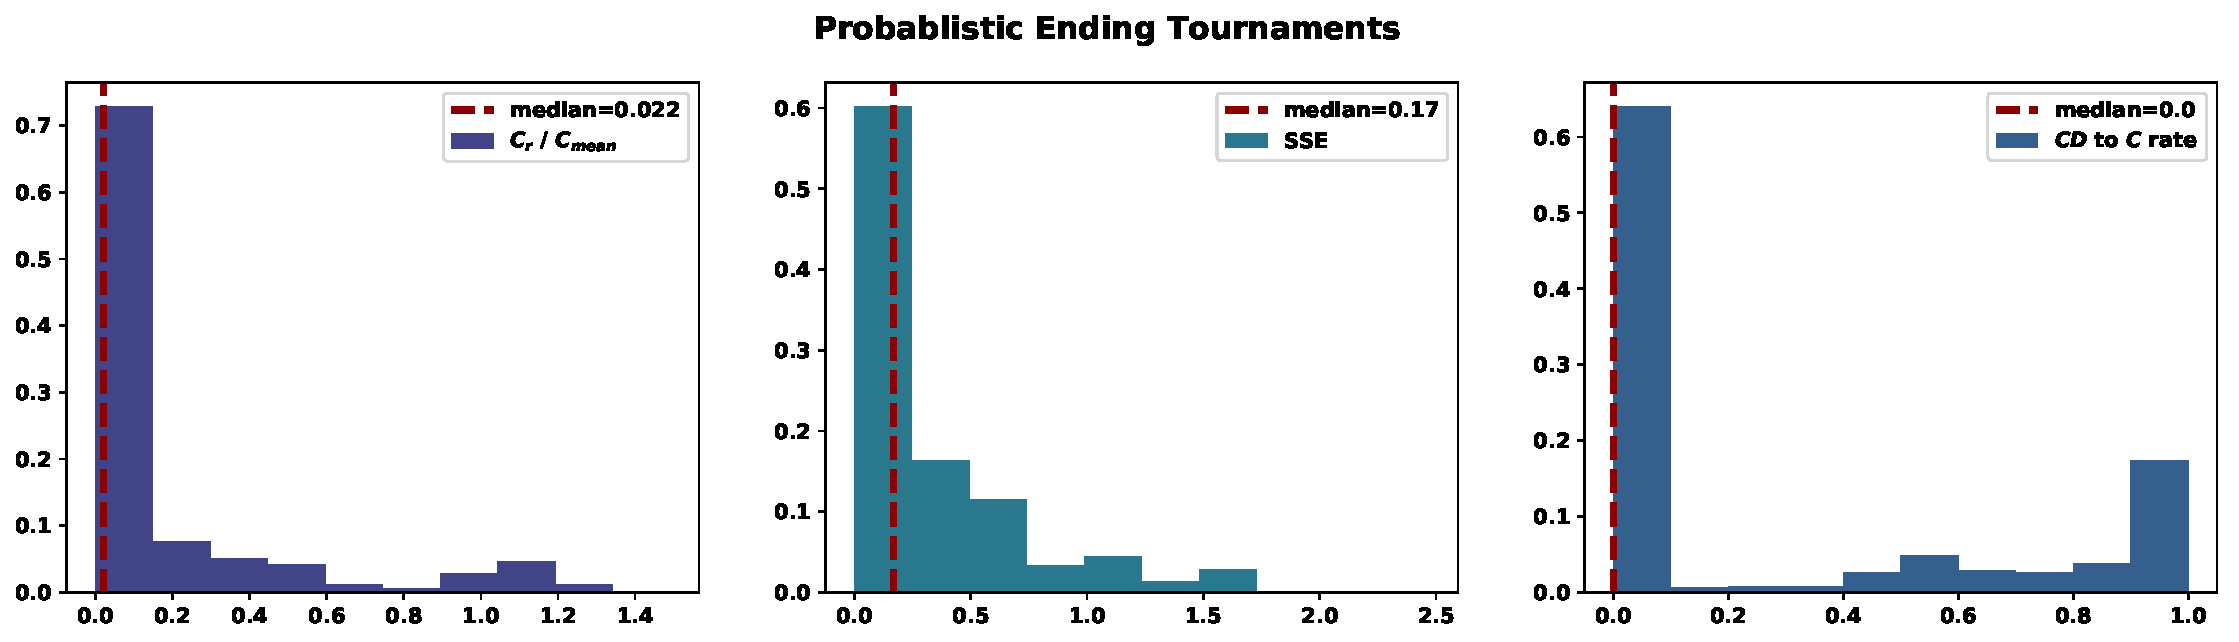
\includegraphics[width=\textwidth]{../images/probend_discussion.pdf}
        \caption{Distributions of \(C_r / C_{\text{mean}}\), SSE and \(CD\) to \(C\) ratio
        for the winners of probabilistic ending tournaments.}
        \label{fig:discussion_probend}
\end{figure}

The distributions of the \(CD\) to \(C\) rate evaluate the behaviour of a
successful strategy after its opponent has defected against it. In standard
tournaments it was observed that a successful strategy reciprocates with a
probability of 0.5, and in a setting that the type
of the tournament can vary between all the examined types a winning strategy
would reciprocate on average with a probability of 0.58. In
tournaments with noise a strategy is less likely to cooperate following a
defection compared to standard tournaments, and in probabilistic ending
tournaments a strategy will reciprocate a defection.
This leads to adjusting the recommendation of being provocable to defections made
by Axerlod. A strategy should be provocable in tournaments with short matches,
but in the rest of the settings a strategy should be more generous.

\begin{figure}[!htbp]
    \centering
        \centering
        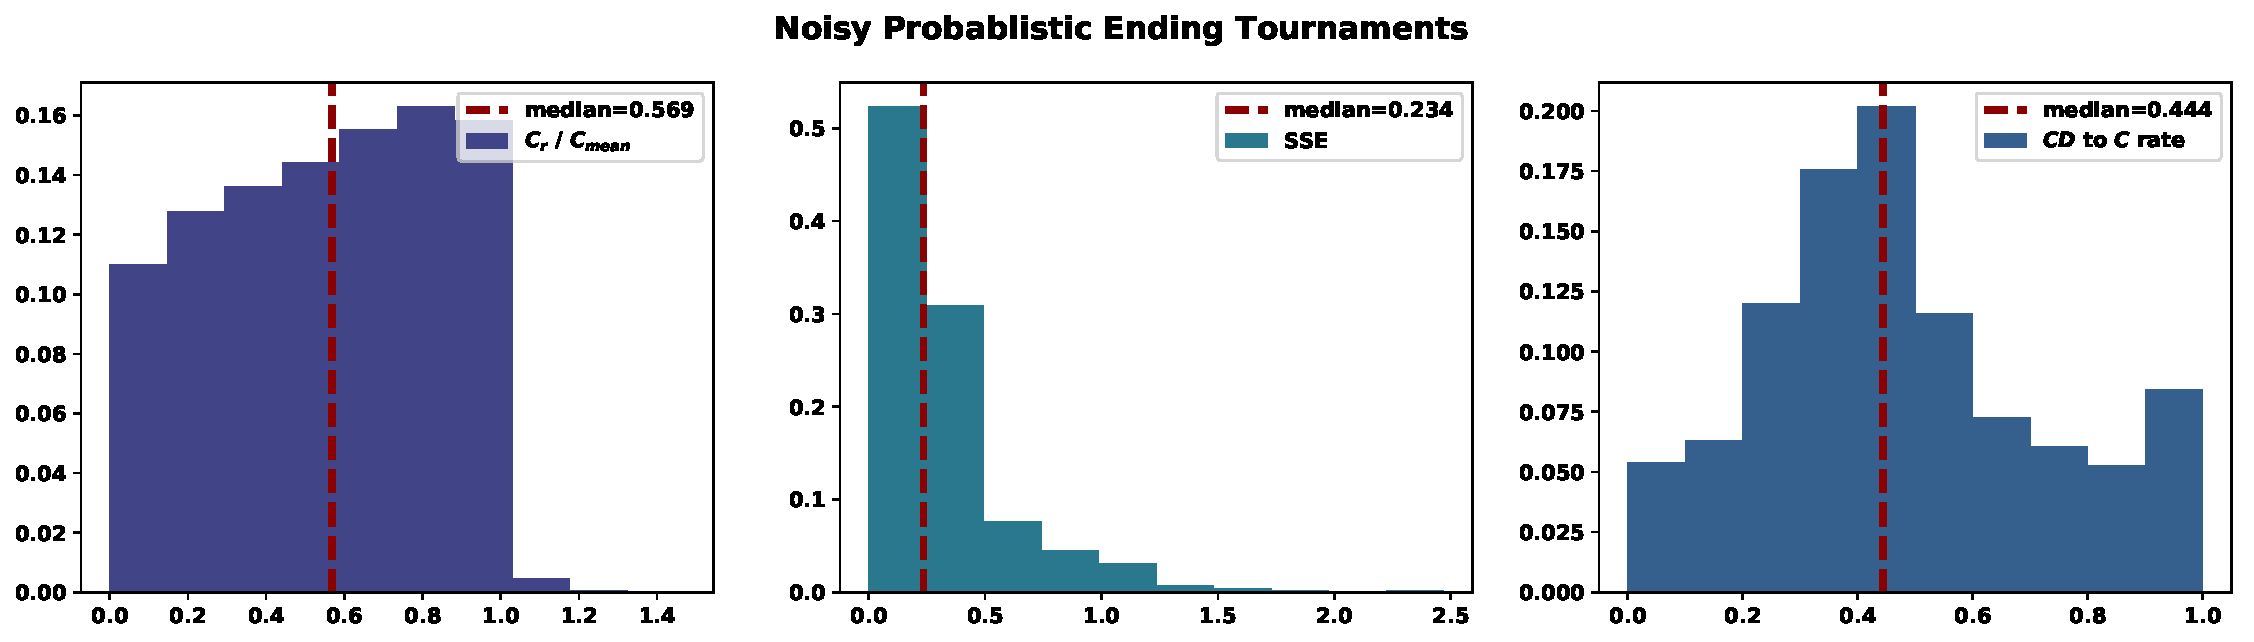
\includegraphics[width=\textwidth]{../images/probend_noisy_discussion.pdf}
        \caption{Distributions of \(C_r / C_{\text{mean}}\), SSE and \(CD\) to \(C\) ratio
        for the winners of noisy probabilistic ending tournaments.}
        \label{fig:discussion_probend_noisy}
\end{figure}

Further statistically significant features with strong effects include \(C_r /
C_{\text{min}}\), \(C_r / C_{\text{max}}\), \(C_{\text{min}}\) and
\(C_{\text{max}}\). These add more emphasis on how important it is for a  a
strategy to adapt to its environment. Finally, the features number of turns,
repetitions and the probabilities of noise and the game ending had no
significant effects based on the multivariate regression models.

\begin{figure}[!htbp]
    \centering
        \centering
        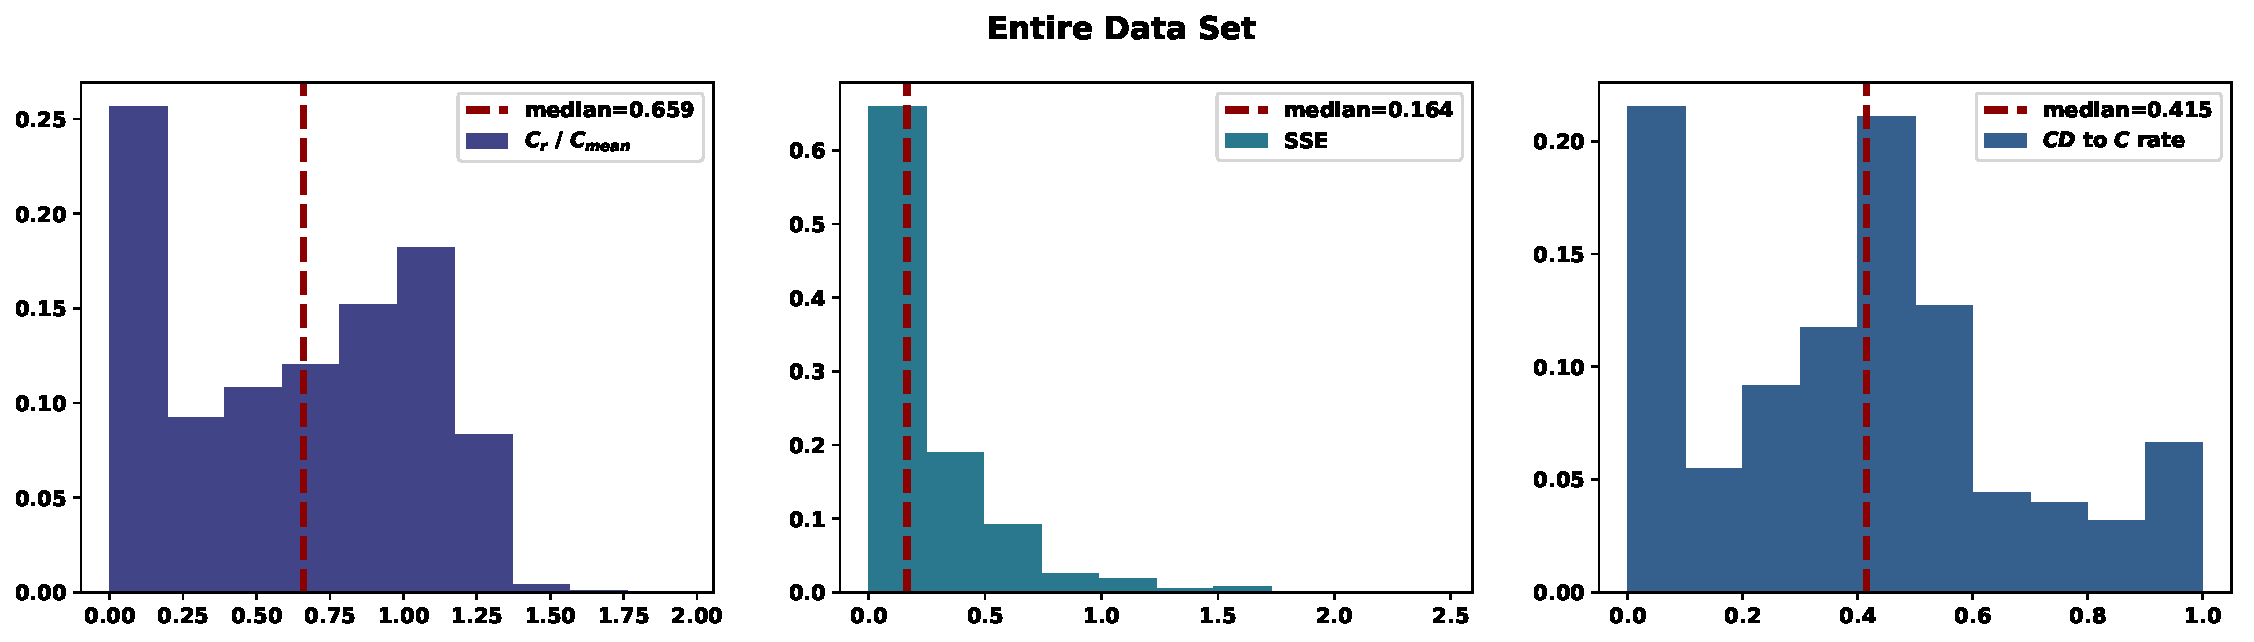
\includegraphics[width=\textwidth]{../images/entire_data_discussion.pdf}
        \caption{Distributions of \(C_r / C_{\text{mean}}\), SSE and \(CD\) to \(C\) ratio
        for the winners over the tournaments of the entire data set.}
        \label{fig:discussion_entire_data}
\end{figure}
\section{Correlation coefficients}\label{app:correlations}

A graphical representation of the correlation coefficients for the features in
Table~\ref{table:manual_features}.

\begin{figure}[!htbp]
        \begin{center}
            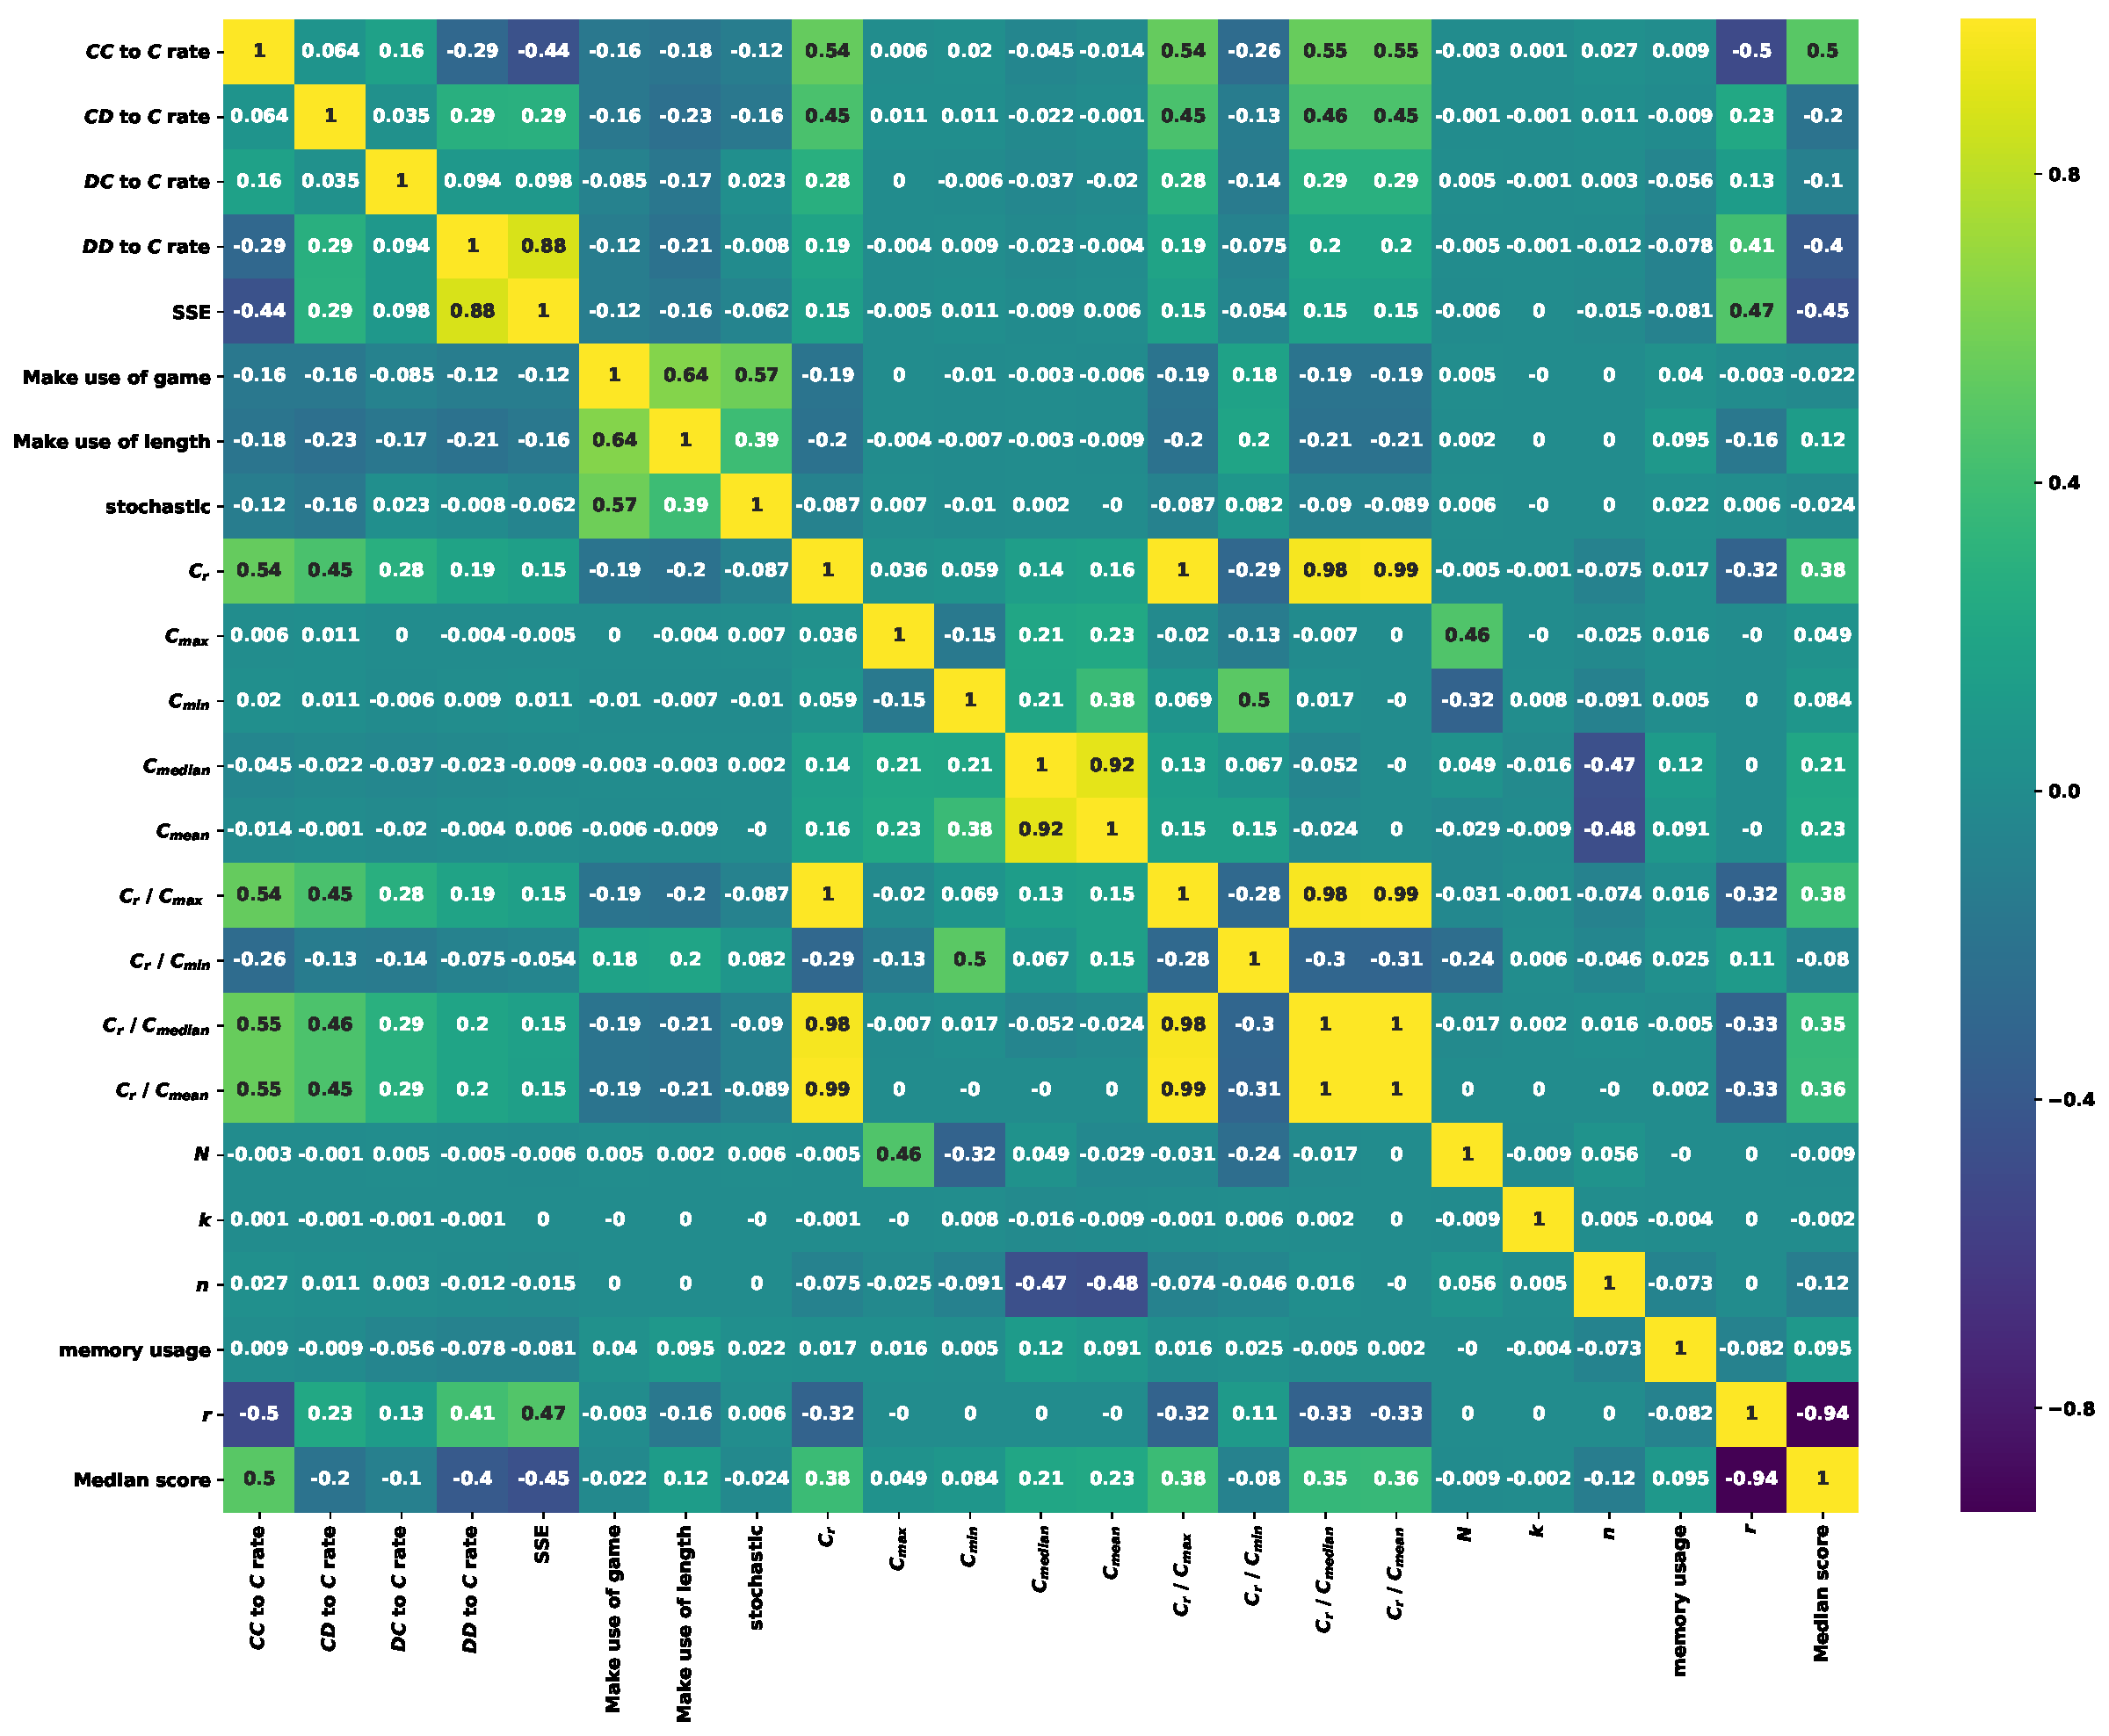
\includegraphics[width=.75\linewidth]{../images/standard_correlation_plot.pdf}
        \end{center}
        \caption{Correlation coefficients of features in Table~\ref{table:manual_features}
        for standard tournaments}
\end{figure}
\begin{figure}[!htbp]
    \begin{center}
        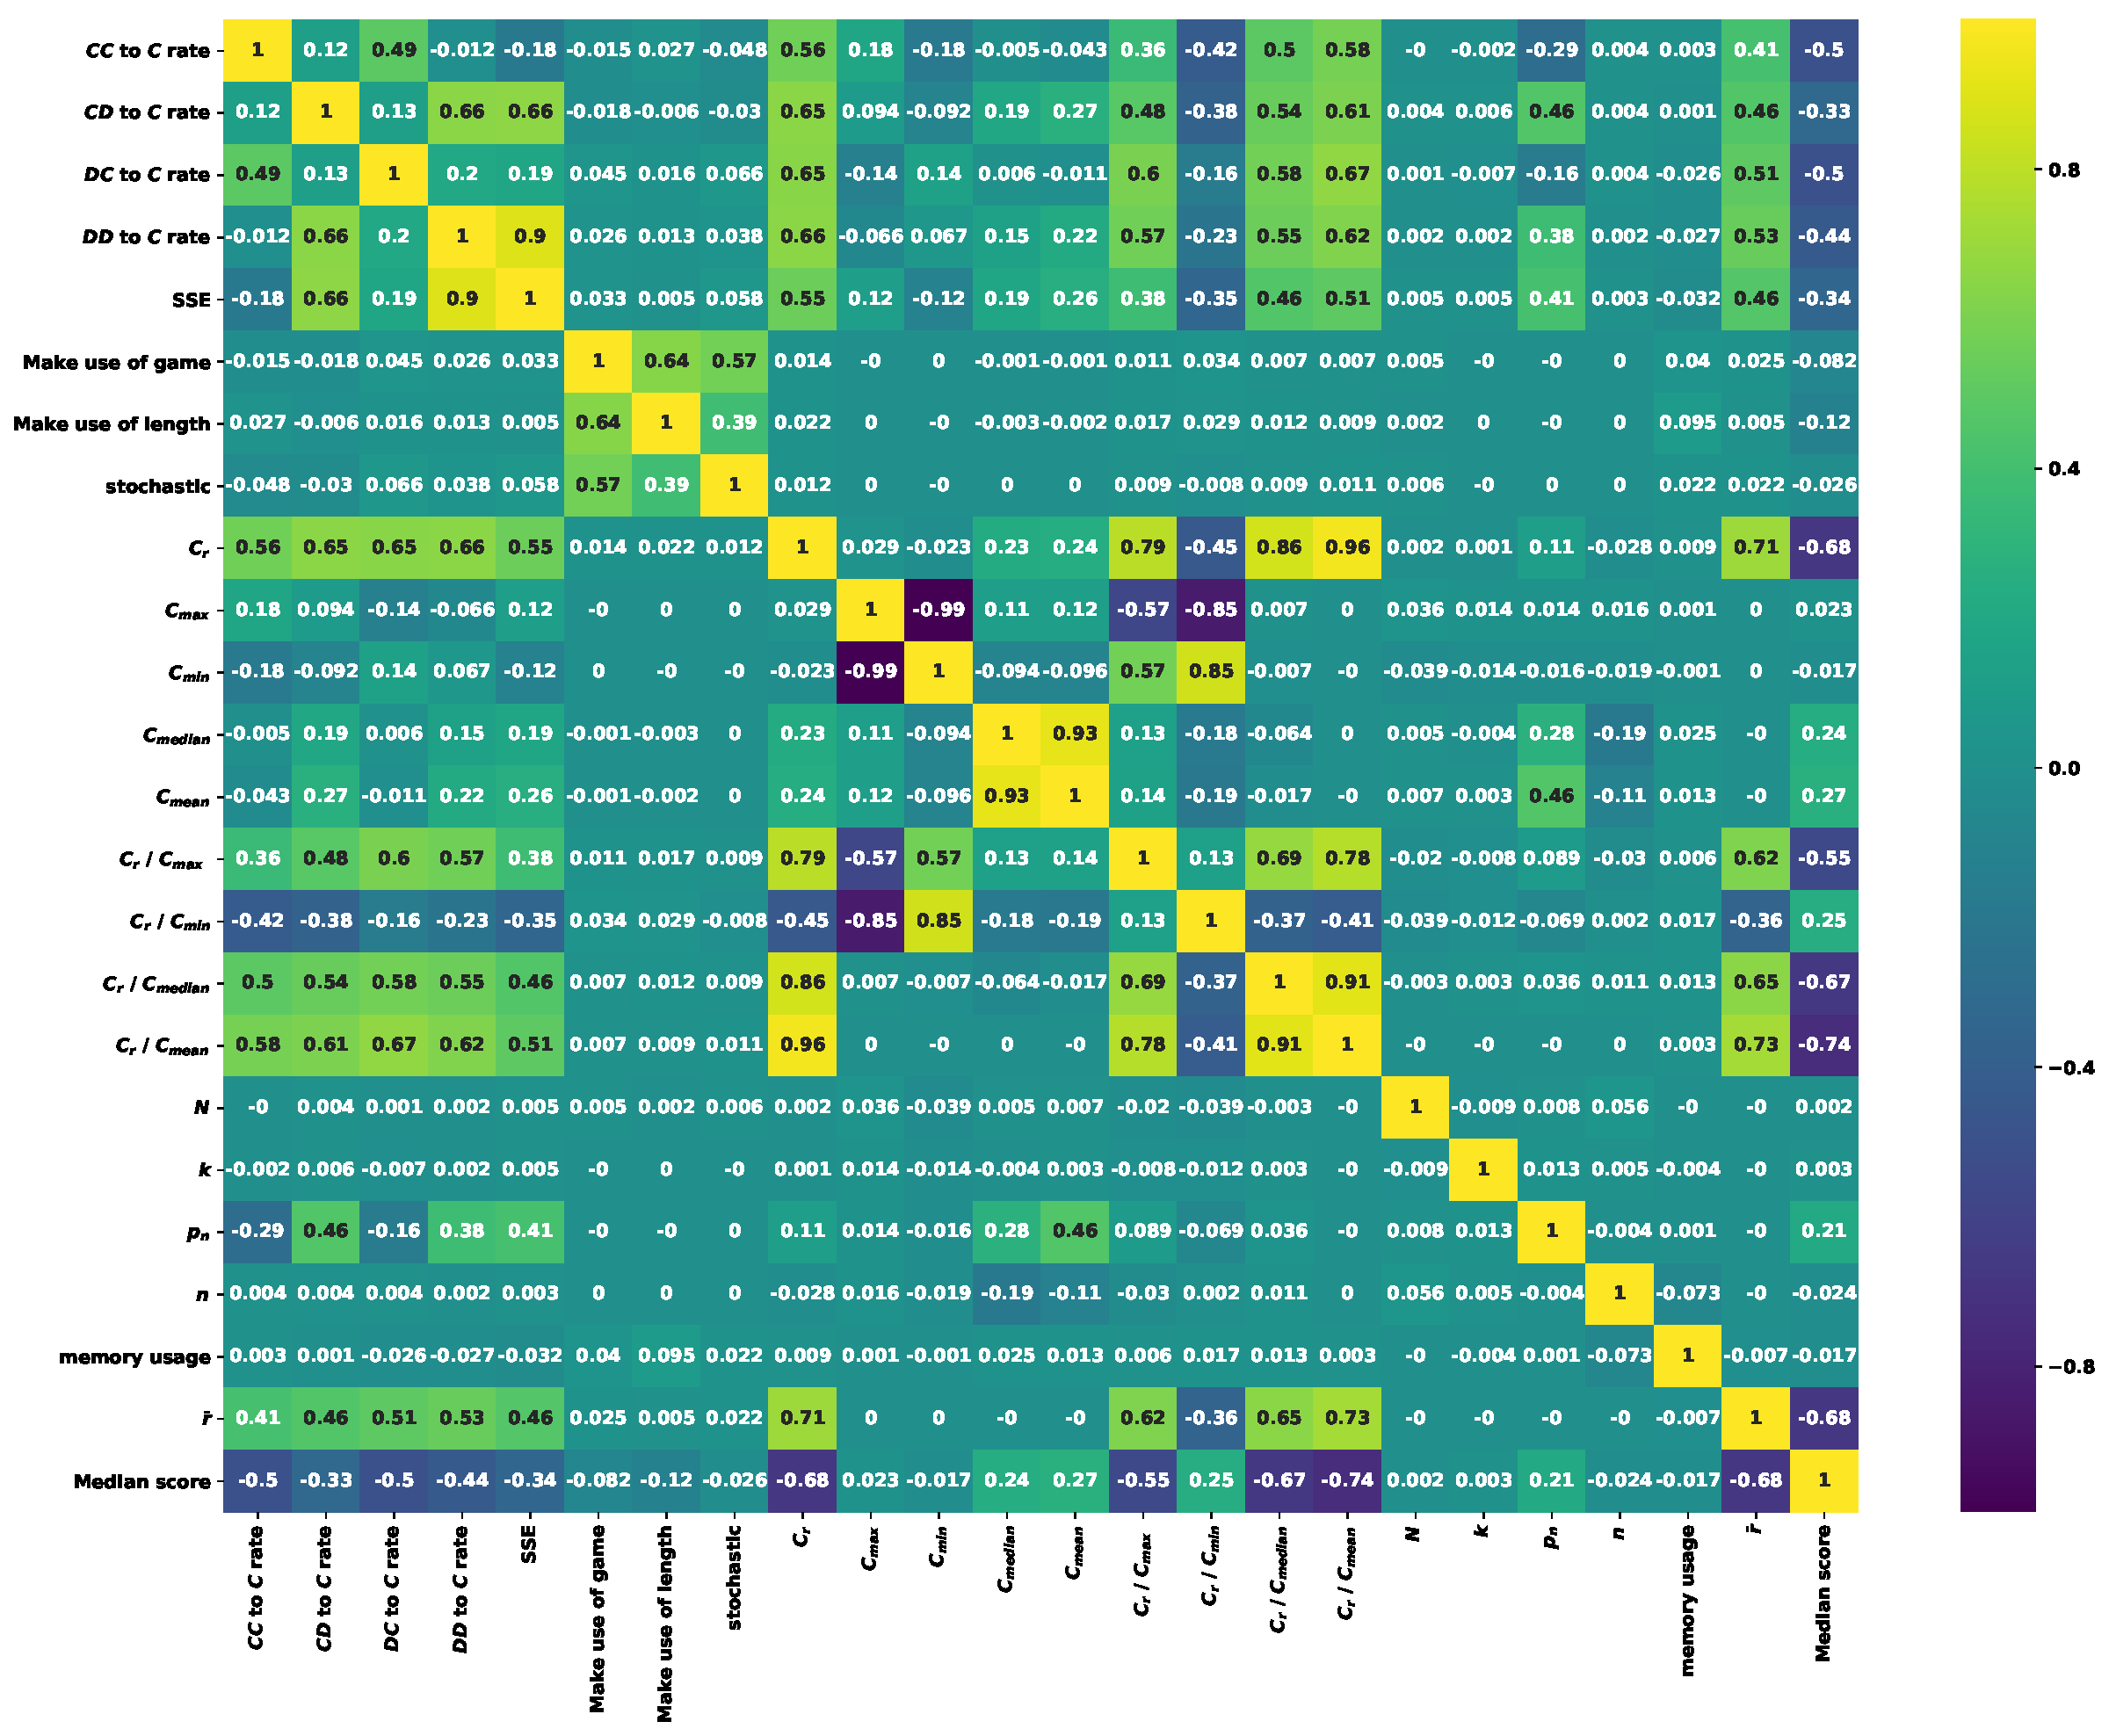
\includegraphics[width=.75\linewidth]{../images/noise_correlation_plot.pdf}
    \end{center}
    \caption{Correlation coefficients of features in Table~\ref{table:manual_features}
    for noisy tournaments}
\end{figure}
\begin{figure}[!htbp]
    \begin{center}
        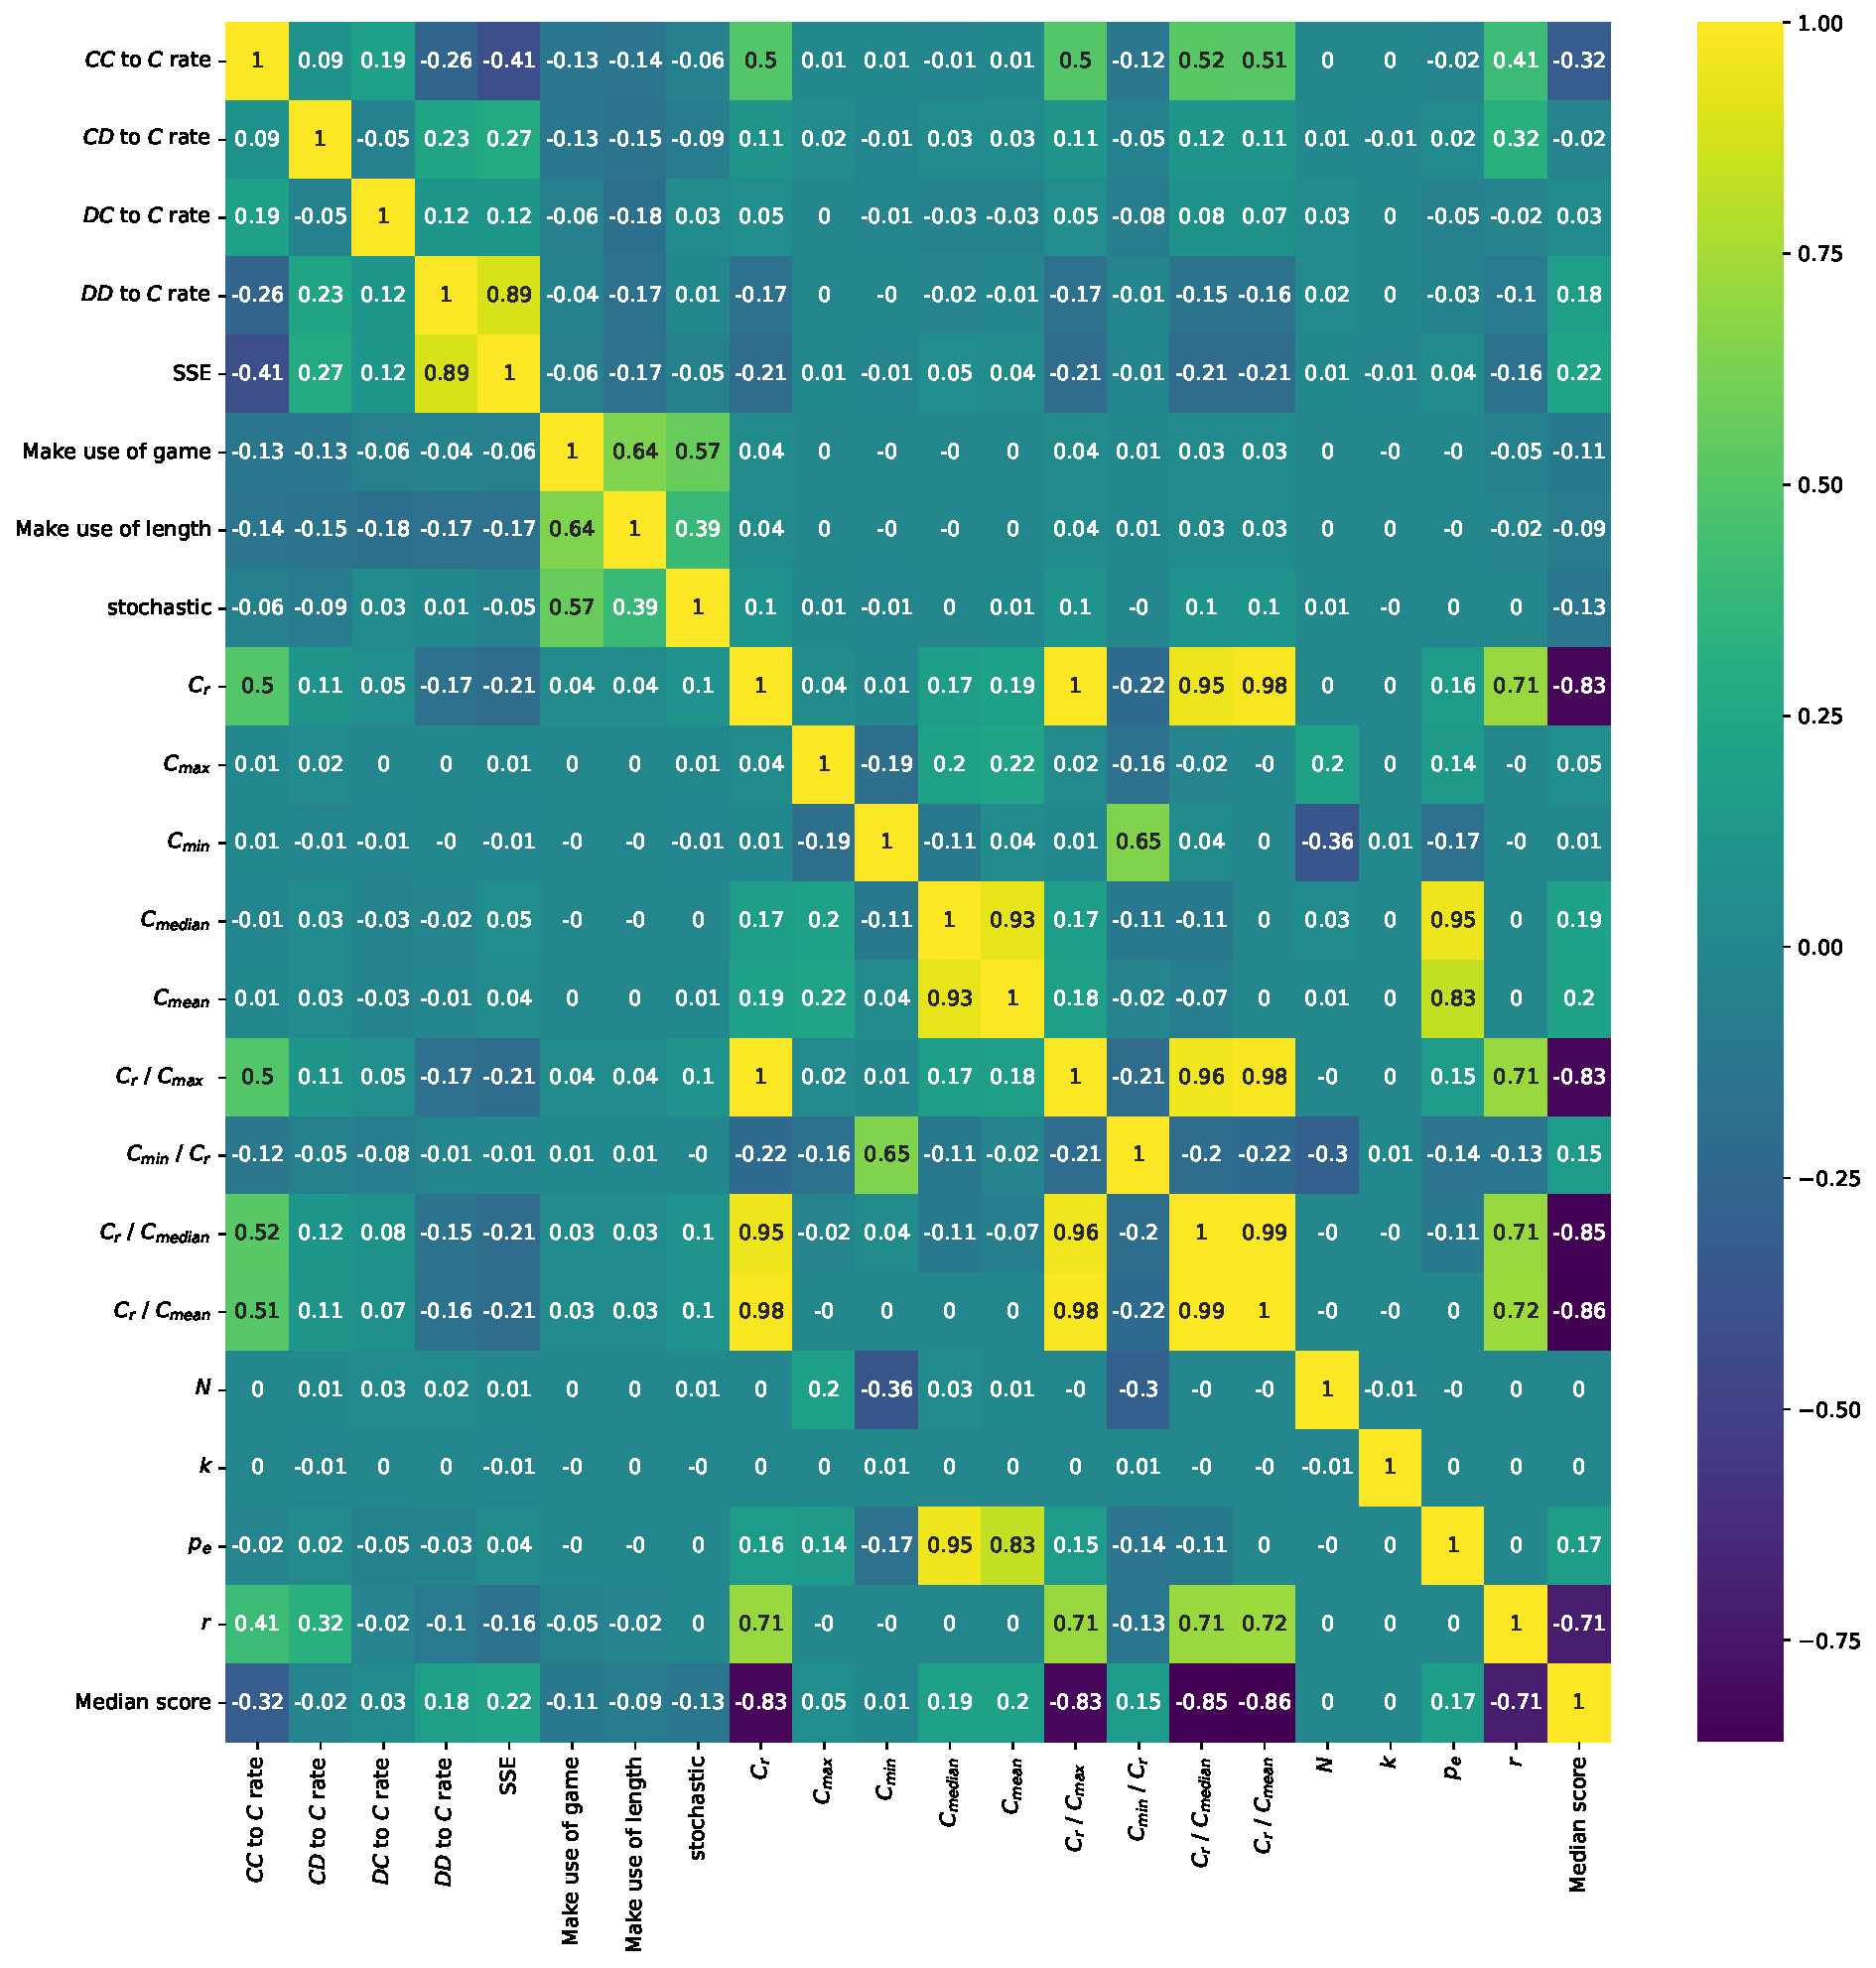
\includegraphics[width=.75\linewidth]{../images/probend_correlation_plot.pdf}
    \end{center}
    \caption{Correlation coefficients of features in Table~\ref{table:manual_features}
    for probabilistic ending tournaments}
\end{figure}
\begin{figure}[!htbp]
    \begin{center}
        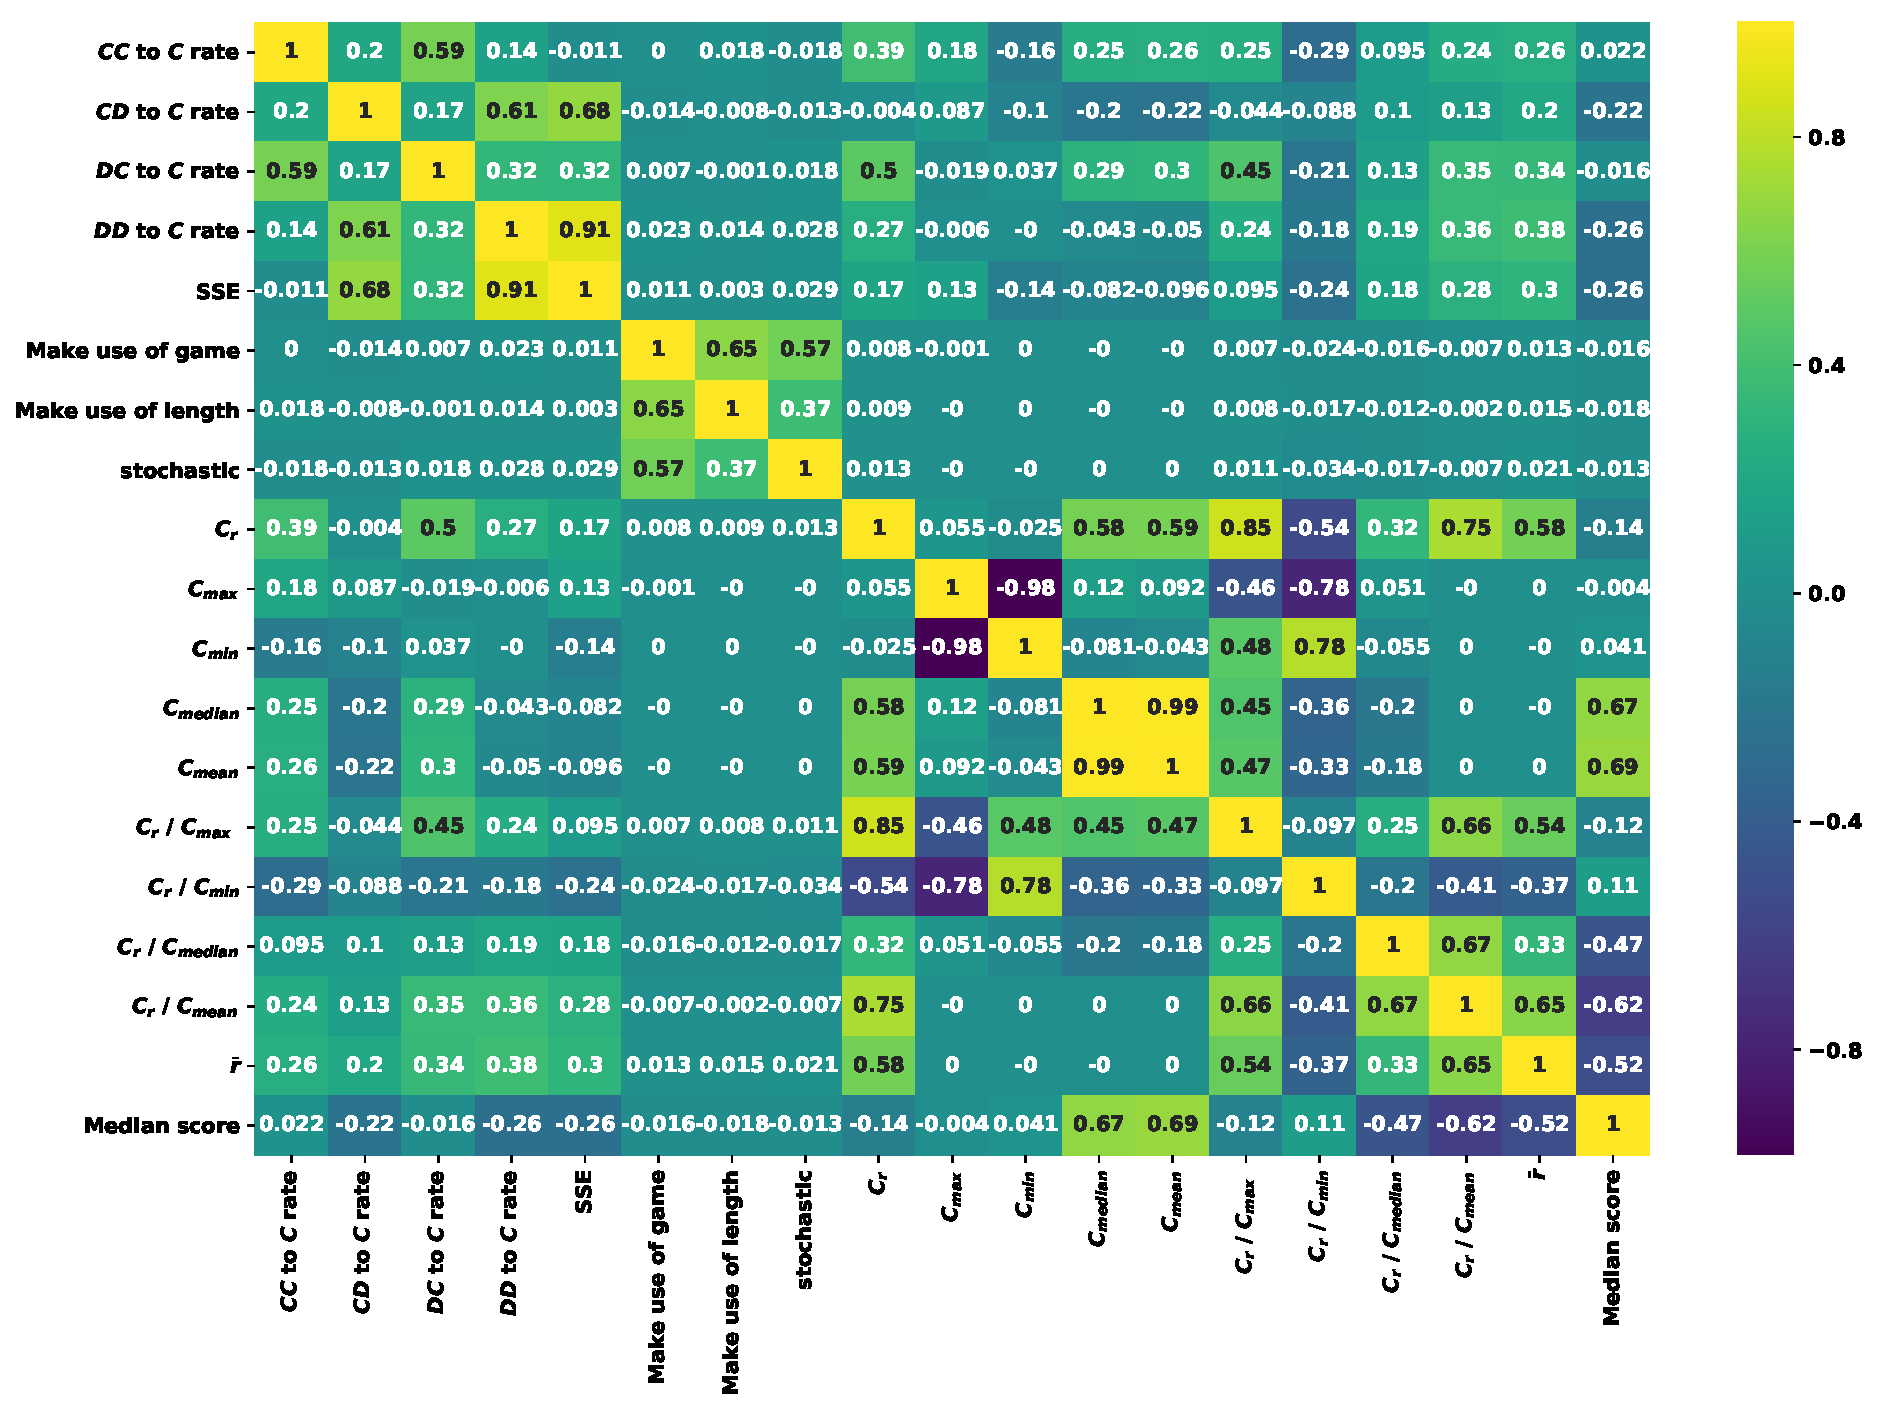
\includegraphics[width=.75\linewidth]{../images/probend_noise_correlation_plot.pdf}
    \end{center}
    \caption{Correlation coefficients of features in Table~\ref{table:manual_features}
    for noisy probabilistic ending tournaments}
\end{figure}
\begin{figure}[!htbp]
    \begin{center}
        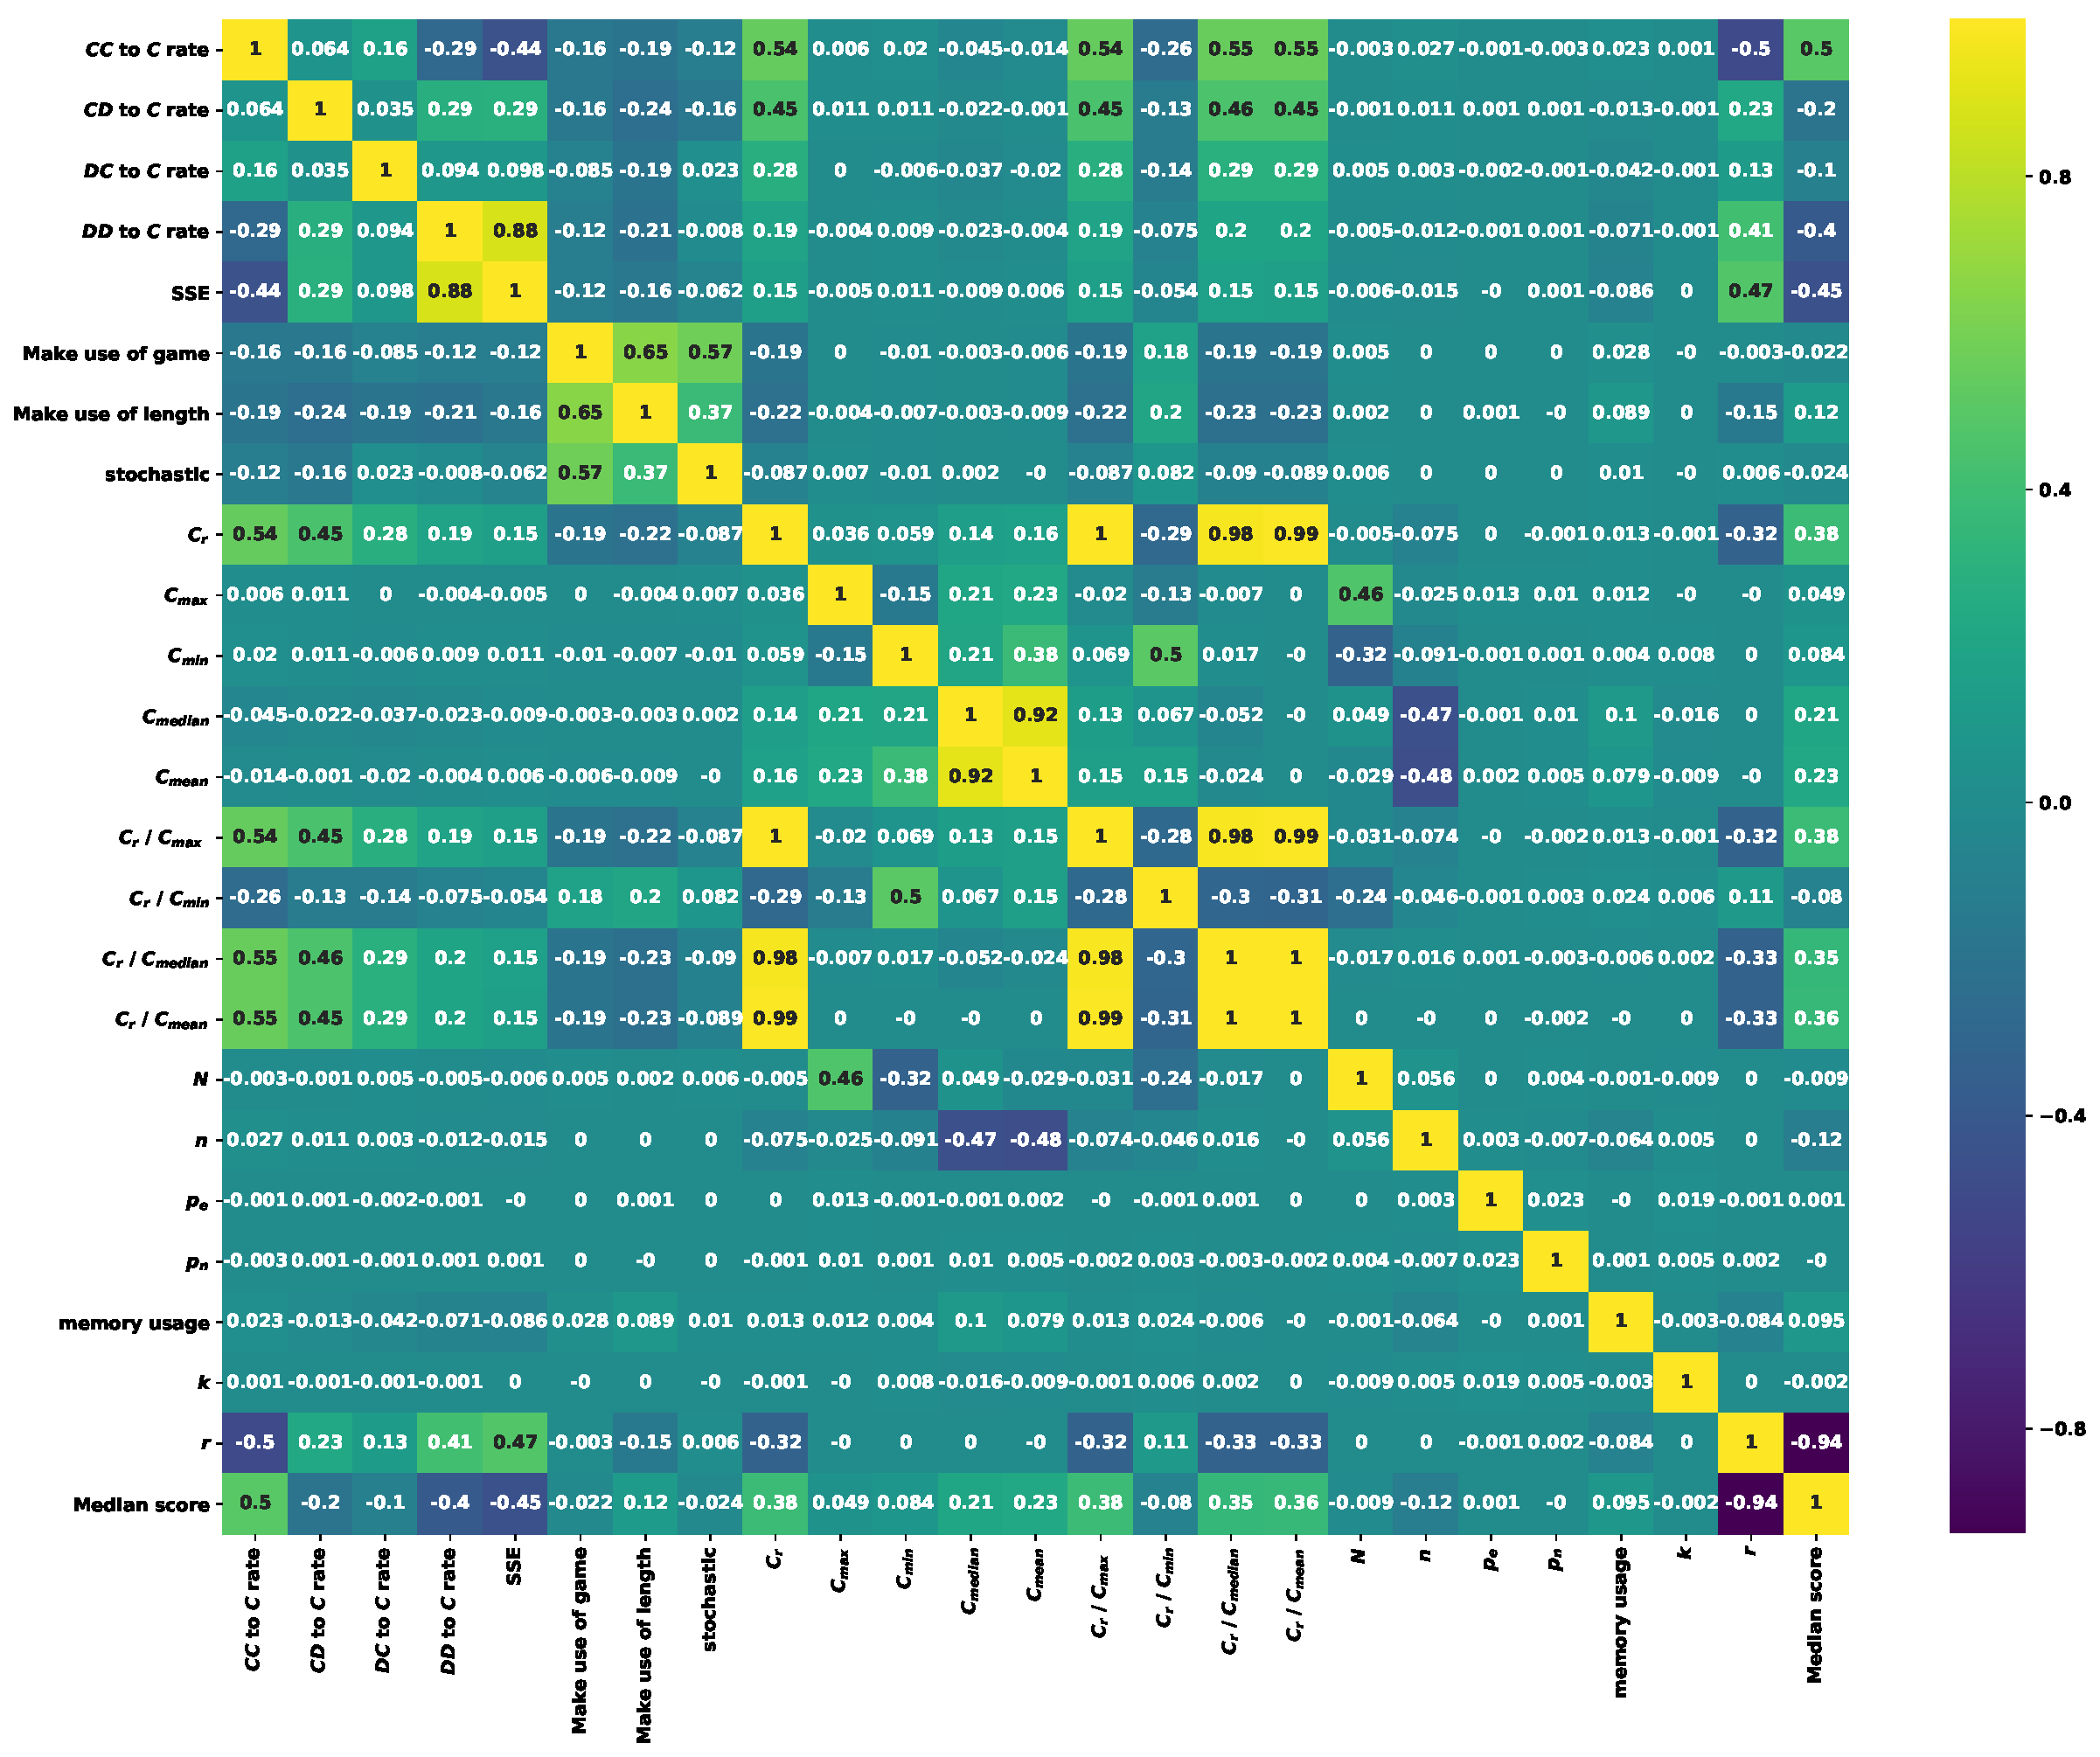
\includegraphics[width=.75\linewidth]{../images/merged_correlation_plot.pdf}
    \end{center}
    \caption{Correlation coefficients of features in Table~\ref{table:manual_features}
    for data set}
\end{figure}
\section{Evaluation based on clustering and random forest.}\label{app:clustering}

The final method to evaluate the features importance in a strategy's success
is a combination of a clustering task and a random forest algorithm.
Initially the performances are clustered into different clusters
based on them being successful or not. The performances are clustered into
successful and unsuccessful clusters based on 4 different approaches.
More specifically:

\begin{itemize}
    \item \textbf{Approach 1:} The performances are divided into two clusters based
    on whether their performance was in the top \(5\%\) of their respective tournaments.
    Thus, whether \(r\) was smaller or larger than 0.05.
    \item \textbf{Approach 2:} The performances are divided into two clusters based
    on whether their performance was in the top \(25\%\) of their respective tournaments.
    Thus, whether \(r\) was smaller or larger than 0.25.
    \item \textbf{Approach 3:} The performances are divided into two clusters based
    on whether their performance was in the top \(50\%\) of their respective tournaments.
    Thus, whether \(r\) was smaller or larger than 0.50.
    \item \textbf{Approach 4:} The performances are clustered based on their normalised rank and
    their median score by a \(k-\)means algorithm~\cite{Arthur2007}. The number of
    clusters is not deterministically chosen but it is based on the silhouette
    coefficients~\cite{Rousseeuw1987}.
\end{itemize}

Once the performances have been assigned to a cluster for each approach a
random forest algorithm~\cite{breiman2001} is applied. The problem is a supervised
problem where the random forest algorithm predicts the cluster to which a performance
has been assigned to using the features of Table~\ref{table:manual_features}.
The random
forest models are trained on a training set of 70\% of the tournaments results.
The accuracy of each model based on $R^2$ and the number of clusters for each
tournament type (because in the case of Approach 4 it is not
deterministically chosen) are given by Table~\ref{table:accuracy_random_forest}.
The out of the bag error (OOB)~\cite{hastie2005} has also been calculated. The
models fit well, and a high value of both the accuracy measures on the test data
and the OOB error indicate that the model is not over fitting.

\begin{table}[!htbp]
    \begin{center}
        \resizebox{.9\textwidth}{!}{
        \begin{tabular}{lccccc}
    \toprule
    Tournament type & Clustering Approach & Number of clusters & $R^2$ training data &  $R^2$ test data  & $R^2$ OOB score\\
    \midrule
    standard  & Approach 1  & 2 & 0.998831  & 0.987041    & 0.983708 \\
              & Approach 2  & 2 & 0.998643  & 0.978626    & 0.969202 \\
              & Approach 3  & 2 & 0.998417  & 0.985217    & 0.976538 \\
              & Approach 4  & 2 & 0.998794  & 0.990677    & 0.982959 \\
    \midrule
    noisy     & Approach 1  & 2 & 0.997786  & 0.972229    & 0.968332\\
              & Approach 2  & 2 & 0.997442  & 0.963254    & 0.955219\\
              & Approach 3  & 2 & 0.997152  & 0.953164    & 0.940528\\
              & Approach 4  & 3 & 0.996923  & 0.950728    & 0.935444\\
    \midrule
    probabilistic ending & Approach 1 & 2 & 0.997909   & 0.981490  & 0.978120 \\
                         & Approach 2 & 2 & 0.997883   & 0.973492  & 0.967150 \\
                         & Approach 3 & 2 & 0.990448   & 0.890068  & 0.875822 \\
                         & Approach 4 & 2 & 0.999636   & 0.995183  & 0.992809 \\
    \midrule
    noisy probabilistic ending & Approach 1  & 2 & 0.995347 & 0.957846   & 0.952353\\
                               & Approach 2  & 2 & 0.992813 & 0.909346   & 0.898613\\
                               & Approach 3  & 2 & 0.990579 & 0.824794   & 0.806540\\
                               & Approach 4  & 4 & 0.989465 & 0.841652   & 0.824052\\
    \midrule
    over \numberofalltournaments tournaments   & Approach 1 & 2 & 0.997271& 0.972914& 0.969198 \\
                                               & Approach 2 & 2 & 0.996323& 0.951194& 0.940563 \\
                                               & Approach 3 & 2 & 0.993707& 0.906941& 0.891532 \\
                                               & Approach 4 & 3 & 0.993556& 0.913335& 0.898453 \\
    \bottomrule
        \end{tabular}}
    \end{center}
    \caption{Accuracy metrics for random forest models.}
    \label{table:accuracy_random_forest}
\end{table}

The importance that the features of Table~\ref{table:manual_features} had on
each random forest model are given by Figures~\ref{fig:clustering_importance_standard},
\ref{fig:clustering_importance_noise},~\ref{fig:clustering_importance_probend},
\ref{fig:clustering_importance_probend_noise}
and~\ref{fig:clustering_importance_overall}. These show that the classifiers
stochastic, make use of game and make use of length have no significant effect,
and several of the features that are highlighted by the importance are inline with
the correlation results. Moreover, the smoothing parameter \(k\) appears to no
have a significant effect either. The most important features based on the
random forest analysis were $C_{r} / C_{median}$ and $C_r / C_{mean}$.

\begin{figure}[!htbp]
    \begin{subfigure}[t]{0.5\textwidth}
        \begin{center}
            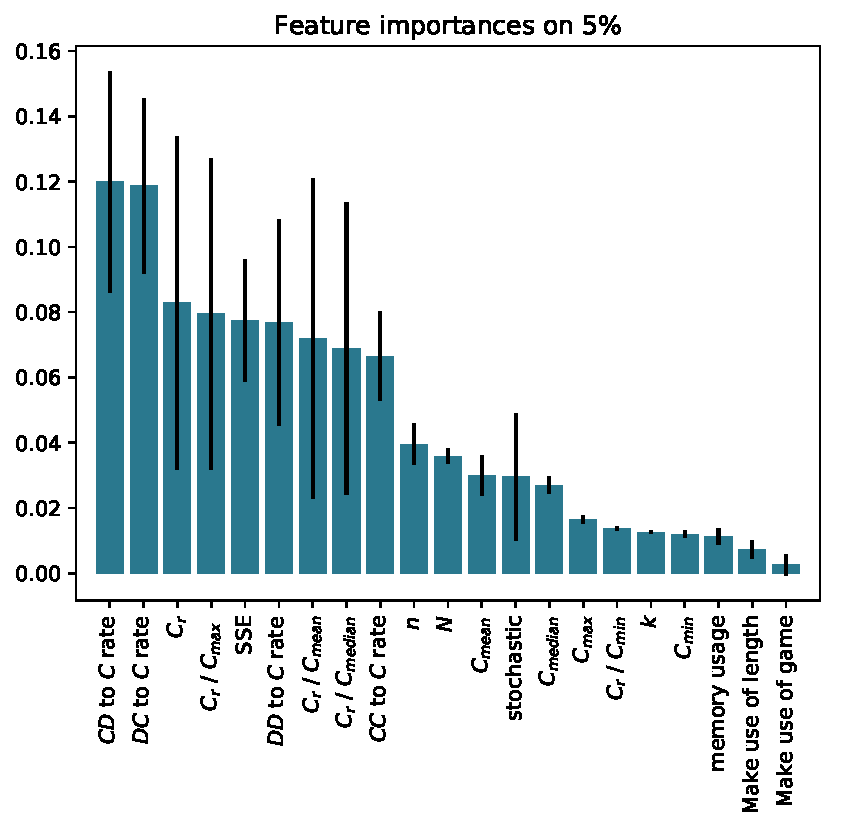
\includegraphics[width=.75\linewidth]{../new_output/standard/_feature_importance_bar_plot_cluster_on_0_05.pdf}
        \end{center}
        \caption{Importance of features for clusters on 5\% performance.}
    \end{subfigure}\hfill
    \begin{subfigure}[t]{0.5\textwidth}
        \begin{center}
            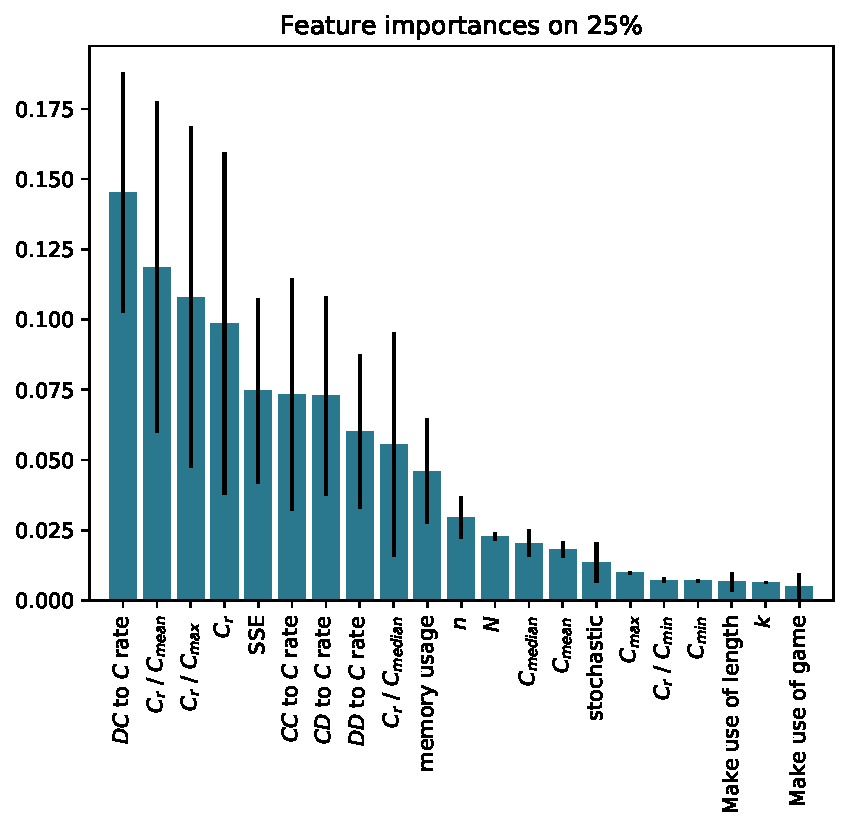
\includegraphics[width=.75\linewidth]{../new_output/standard/_feature_importance_bar_plot_cluster_on_0_25.pdf}
        \end{center}
        \caption{Importance of features for clusters on 25\% performance.}
    \end{subfigure}
    \begin{subfigure}[t]{0.5\textwidth}
        \begin{center}
            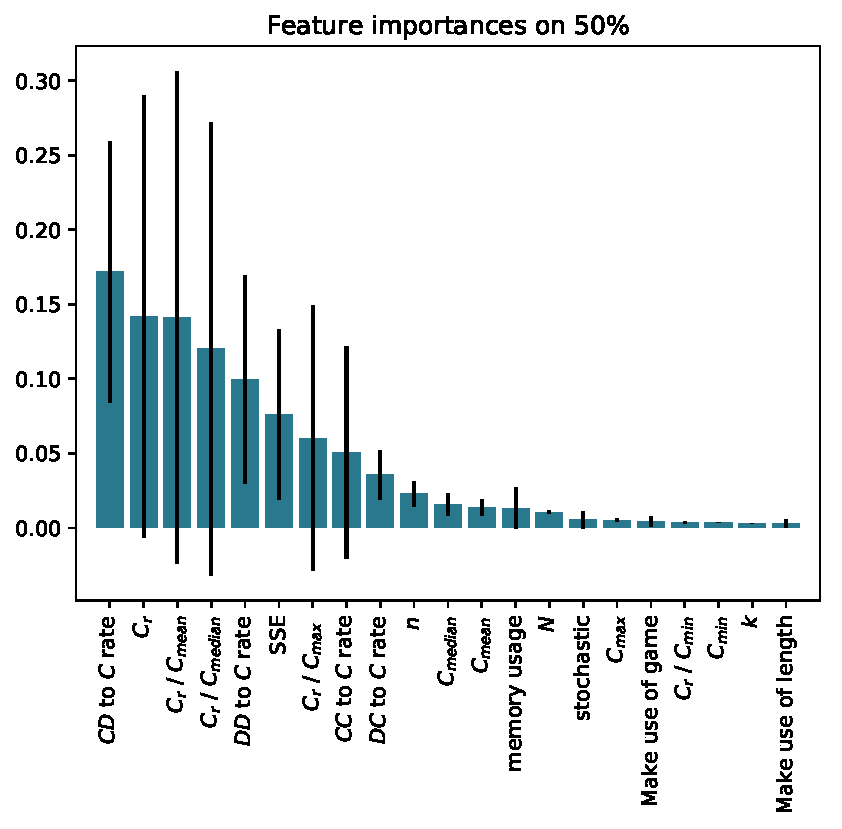
\includegraphics[width=.75\linewidth]{../new_output/standard/_feature_importance_bar_plot_cluster_on_0_5.pdf}
        \end{center}
        \caption{Importance of features for clusters on 50\% performance.}
    \end{subfigure}\hfill
    \begin{subfigure}[t]{0.5\textwidth}
        \begin{center}
            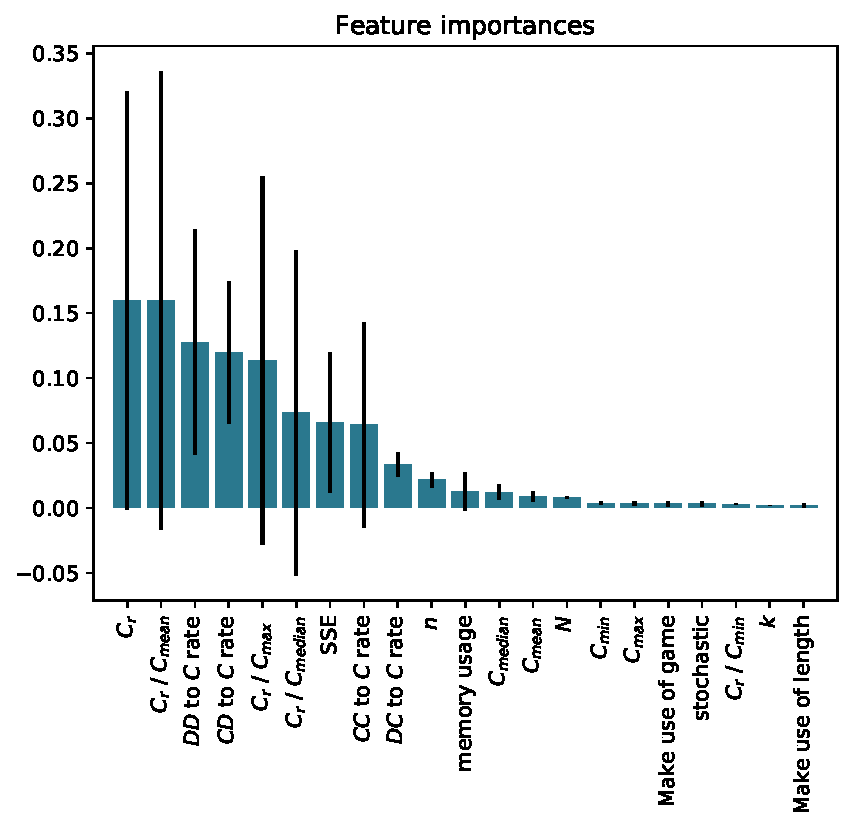
\includegraphics[width=.75\linewidth]{../k_means_output/standard/_feature_importance_bar_plot.pdf}
        \end{center}
        \caption{Importance of features for clusters based on \(k\)means algorithm.}
    \end{subfigure}
    \caption{Importance of features in standard tournaments for different
    clustering methods.}\label{fig:clustering_importance_standard}
\end{figure}

\begin{figure}[!htbp]
    \begin{subfigure}{0.5\textwidth}
        \begin{center}
            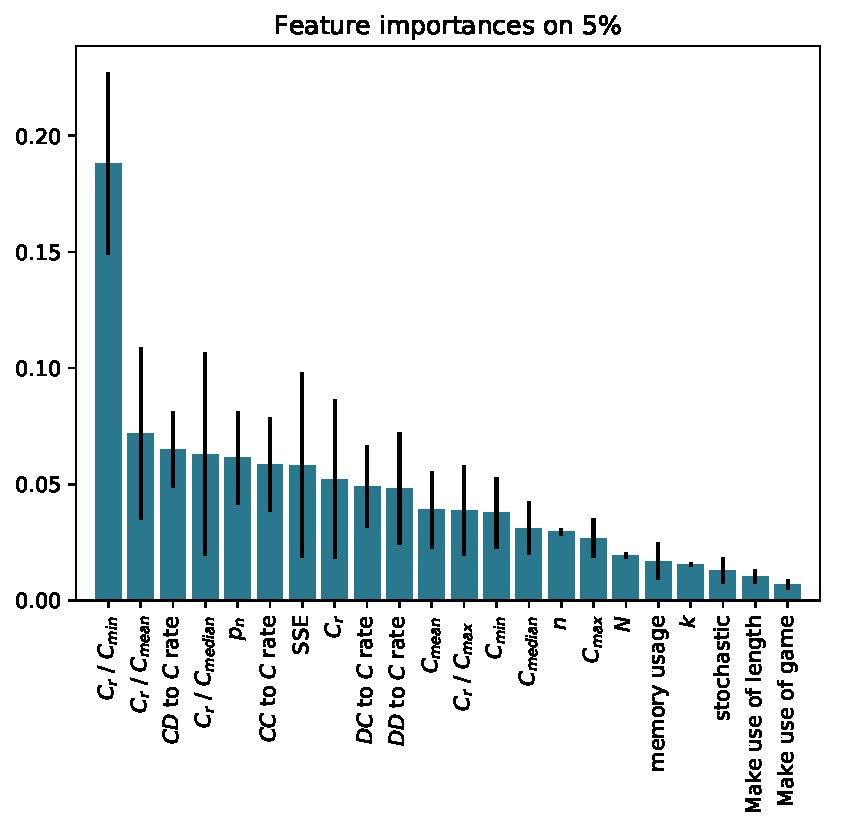
\includegraphics[width=.75\linewidth]{../new_output/noise/_feature_importance_bar_plot_cluster_on_0_05.pdf}
        \end{center}
        \caption{Importance of features for clusters on 5\% performance.}
    \end{subfigure}\hfill
    \begin{subfigure}{0.5\textwidth}
        \begin{center}
            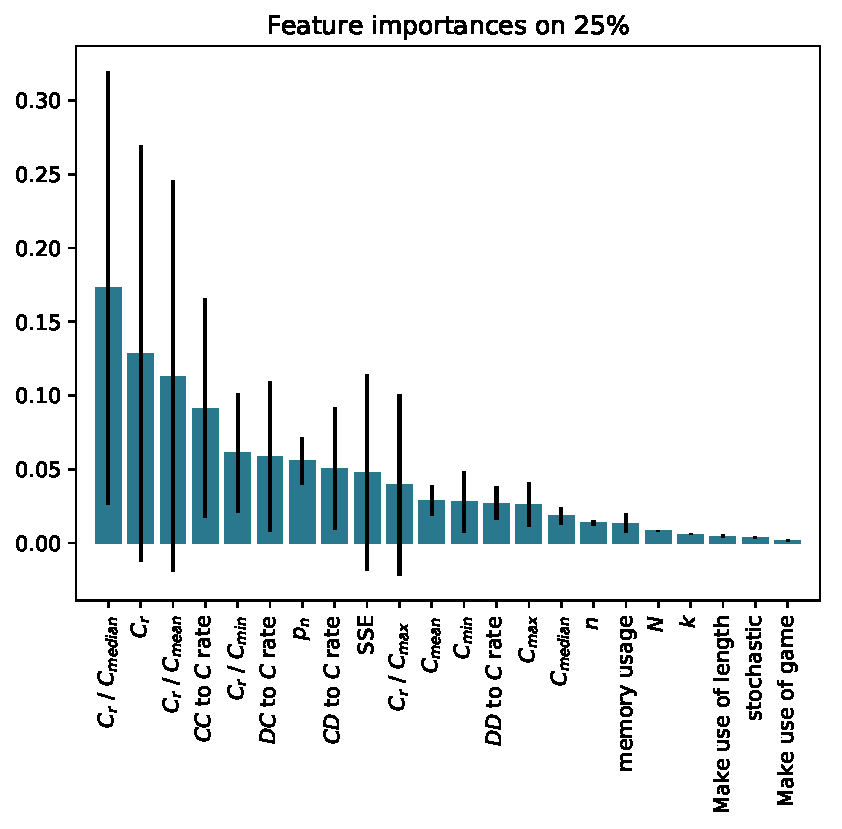
\includegraphics[width=.75\linewidth]{../new_output/noise/_feature_importance_bar_plot_cluster_on_0_25.pdf}
        \end{center}
        \caption{Importance of features for clusters on 25\% performance.}
    \end{subfigure}
    \begin{subfigure}{0.5\textwidth}
        \begin{center}
            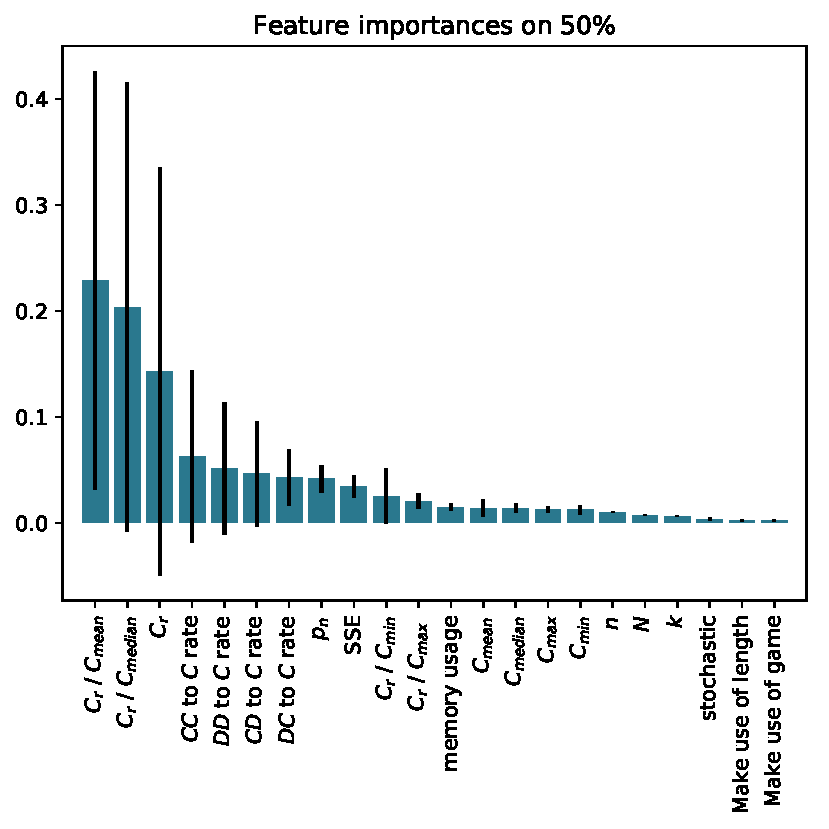
\includegraphics[width=.75\linewidth]{../new_output/noise/_feature_importance_bar_plot_cluster_on_0_5.pdf}
        \end{center}
        \caption{Importance of features for clusters on 50\% performance.}
    \end{subfigure}\hfill
    \begin{subfigure}{0.5\textwidth}
        \begin{center}
            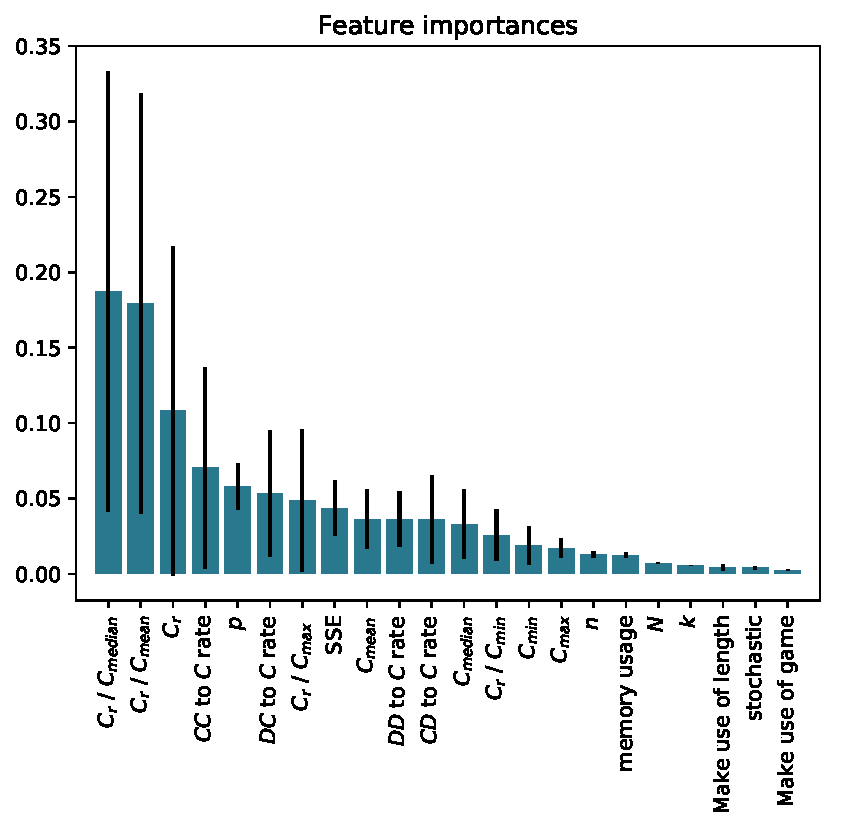
\includegraphics[width=.75\linewidth]{../k_means_output/noise/_feature_importance_bar_plot.pdf}
        \end{center}
        \caption{Importance of features for clusters based on \(k\)means algorithm.}
    \end{subfigure}
    \caption{Importance of features in noisy tournaments for different
    clustering methods.}\label{fig:clustering_importance_noise}
\end{figure}

\begin{figure}[!htbp]
    \begin{subfigure}[t]{0.5\textwidth}
        \begin{center}
            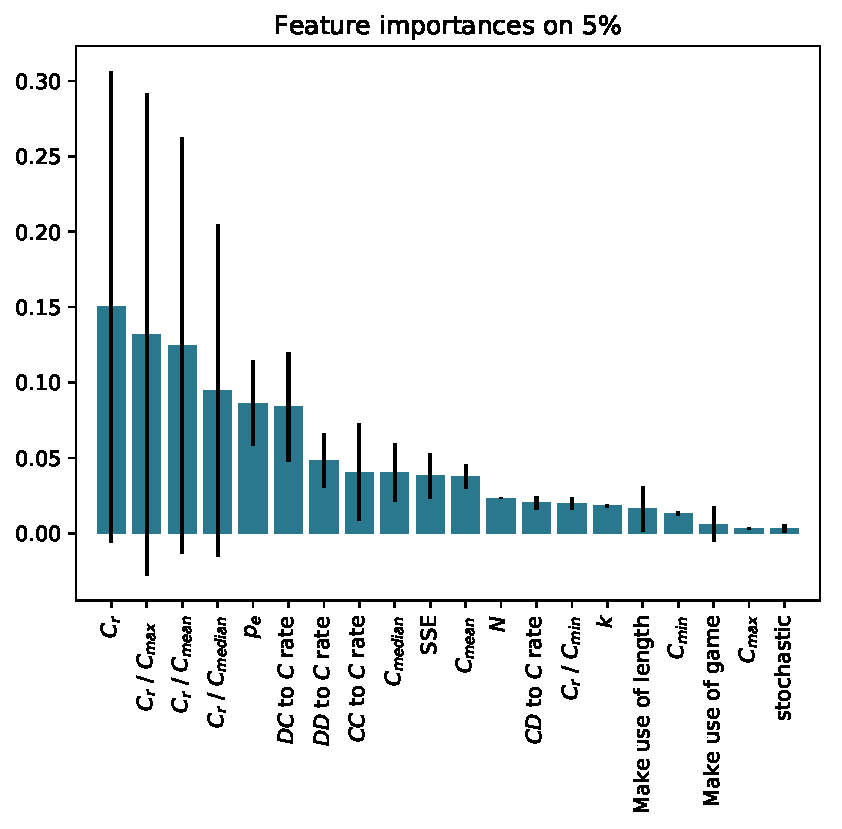
\includegraphics[width=.75\linewidth]{../new_output/probend/_feature_importance_bar_plot_cluster_on_0_05.pdf}
        \end{center}
        \caption{Importance of features for clusters on 5\% performance.}
    \end{subfigure}
    \begin{subfigure}[t]{0.5\textwidth}
        \begin{center}
            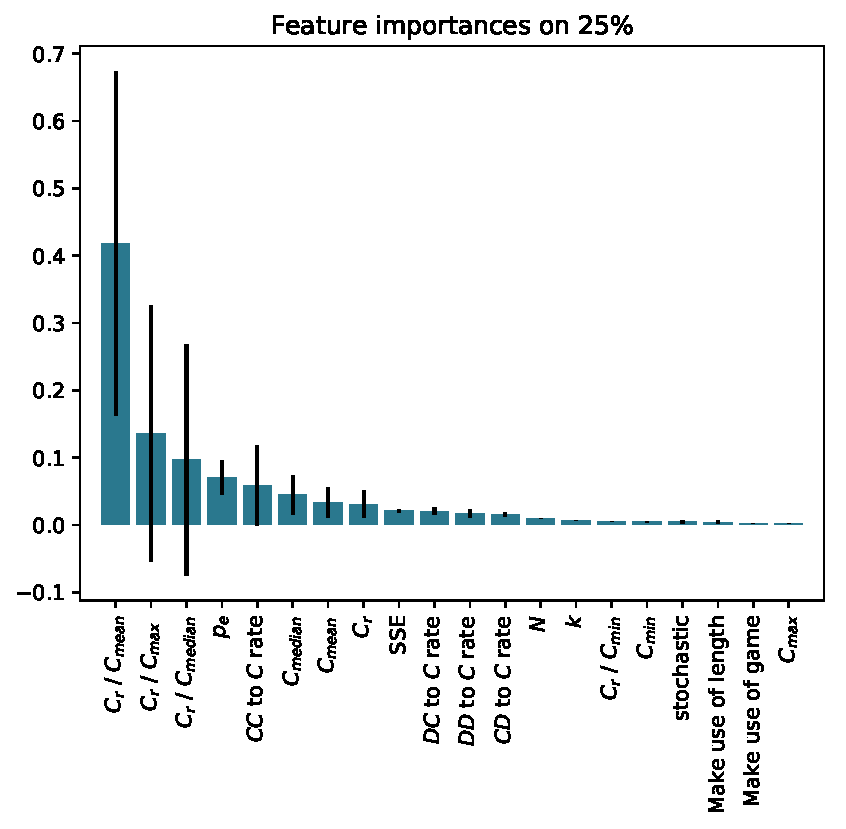
\includegraphics[width=.75\linewidth]{../new_output/probend/_feature_importance_bar_plot_cluster_on_0_25.pdf}
        \end{center}
        \caption{Importance of features for clusters on 25\% performance.}
    \end{subfigure}
    \begin{subfigure}[t]{0.5\textwidth}
        \begin{center}
            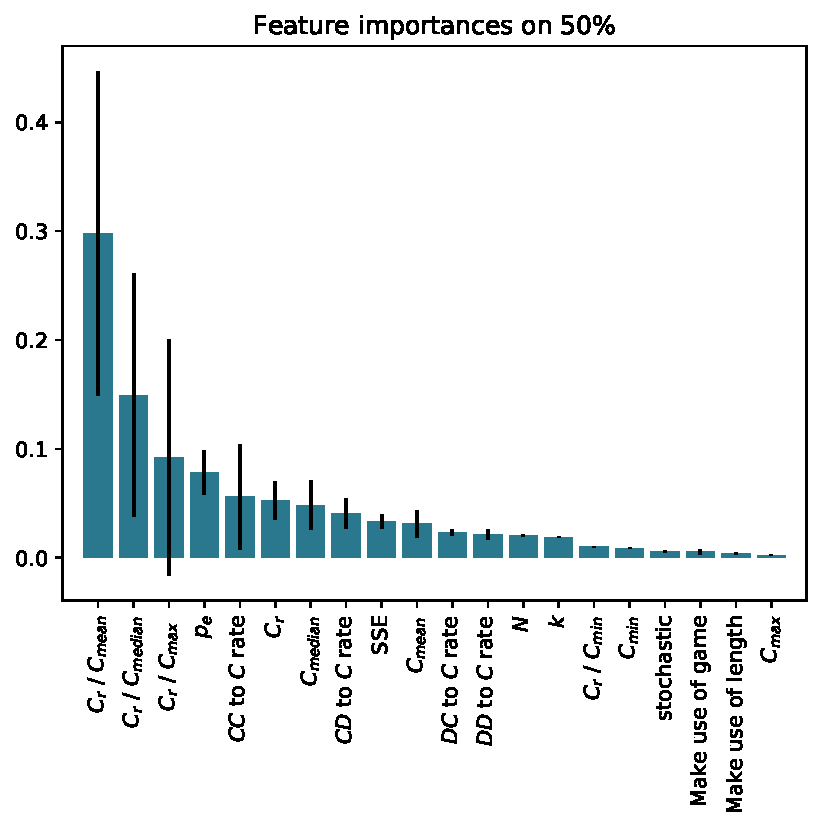
\includegraphics[width=.75\linewidth]{../new_output/probend/_feature_importance_bar_plot_cluster_on_0_5.pdf}
        \end{center}
        \caption{Importance of features for clusters on 50\% performance.}
    \end{subfigure}
    \begin{subfigure}[t]{0.5\textwidth}
        \begin{center}
            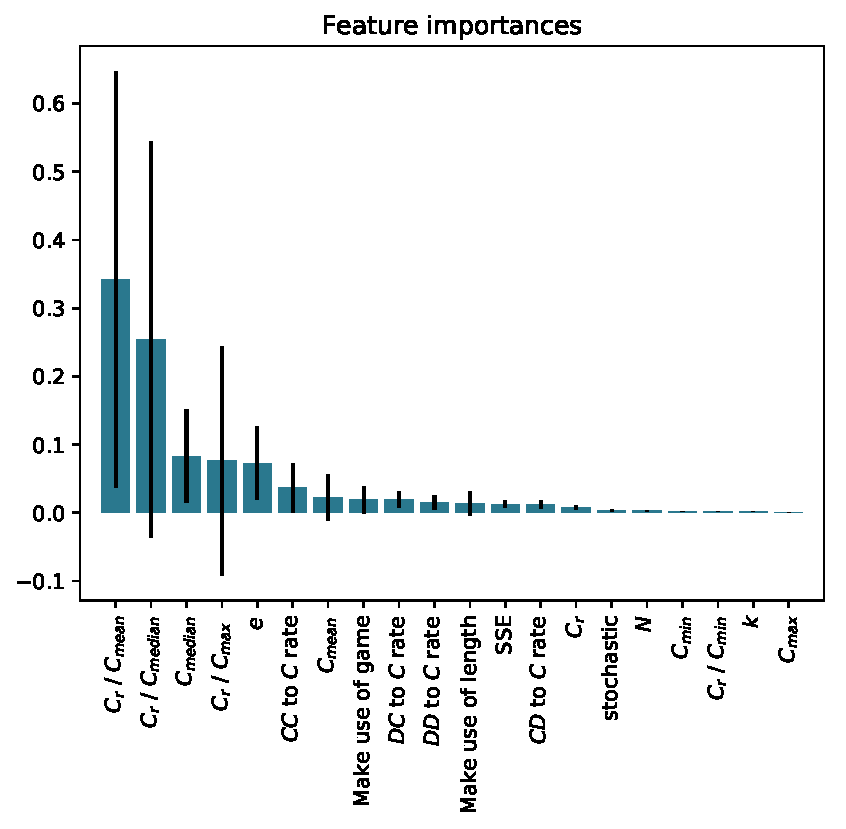
\includegraphics[width=.75\linewidth]{../k_means_output/probend/_feature_importance_bar_plot.pdf}
        \end{center}
        \caption{Importance of features for clusters based on \(k\)means algorithm.}
    \end{subfigure}
    \caption{Importance of features in probabilistic ending tournaments for different
    clustering methods.}\label{fig:clustering_importance_probend}
\end{figure}

\begin{figure}[!htbp]
    \begin{subfigure}[t]{0.5\textwidth}
        \begin{center}
            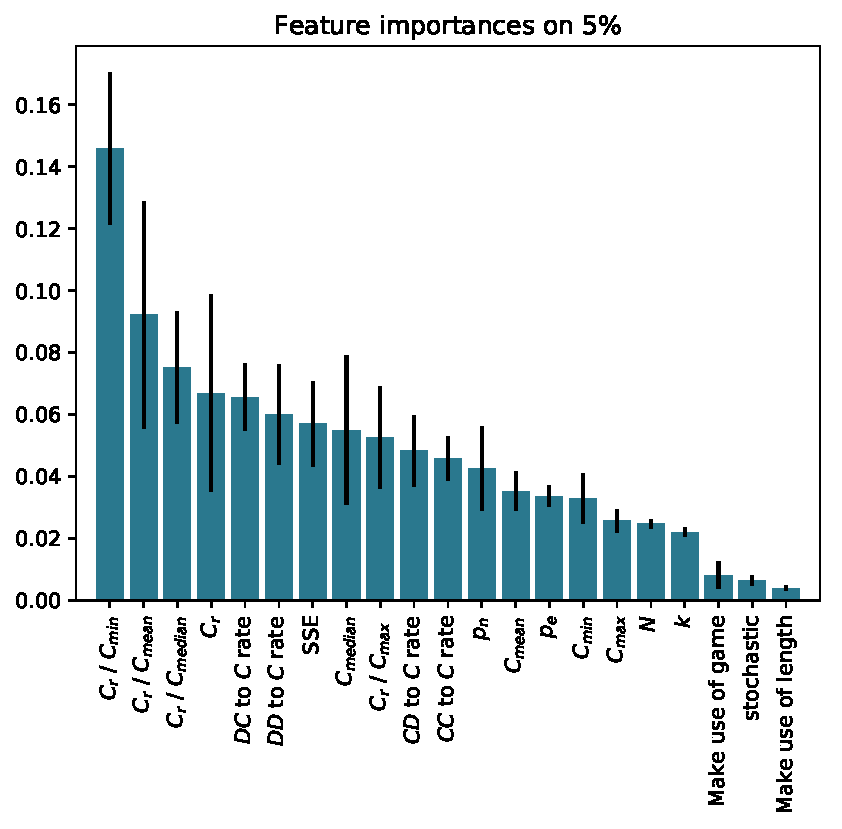
\includegraphics[width=.75\linewidth]{../new_output/probend_noise/_feature_importance_bar_plot_cluster_on_0_05.pdf}
        \end{center}
        \caption{Importance of features for clusters on 5\% performance.}
    \end{subfigure}
    \begin{subfigure}[t]{0.5\textwidth}
        \begin{center}
            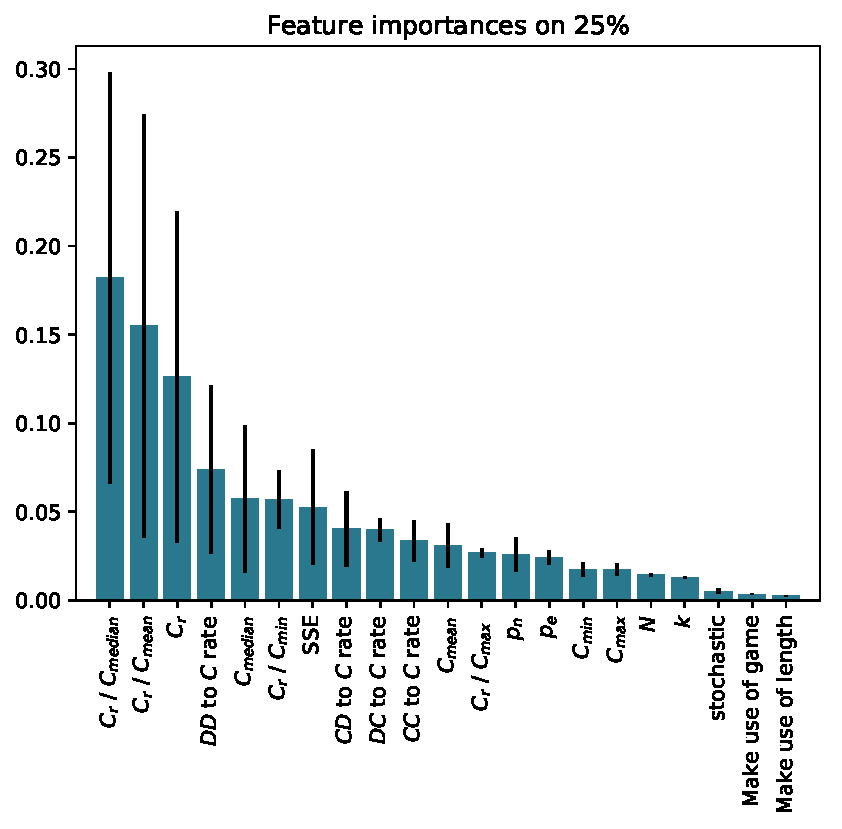
\includegraphics[width=.75\linewidth]{../new_output/probend_noise/_feature_importance_bar_plot_cluster_on_0_25.pdf}
        \end{center}
        \caption{Importance of features for clusters on 25\% performance.}
    \end{subfigure}
    \begin{subfigure}[t]{0.5\textwidth}
        \begin{center}
            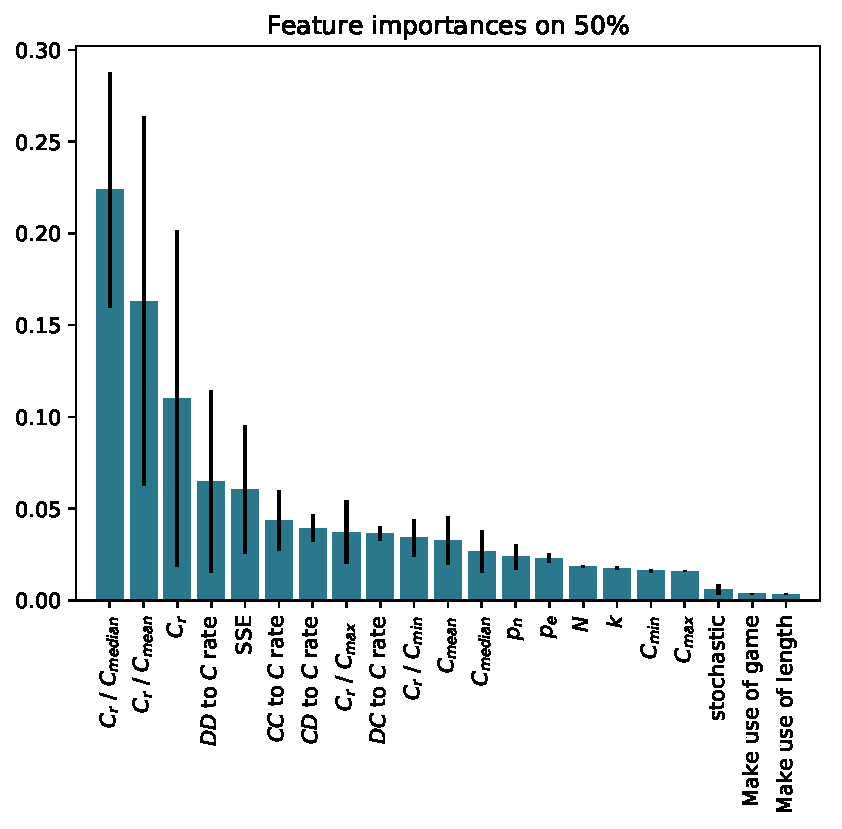
\includegraphics[width=.75\linewidth]{../new_output/probend_noise/_feature_importance_bar_plot_cluster_on_0_5.pdf}
        \end{center}
        \caption{Importance of features for clusters on 50\% performance.}
    \end{subfigure}
    \begin{subfigure}[t]{0.5\textwidth}
        \begin{center}
            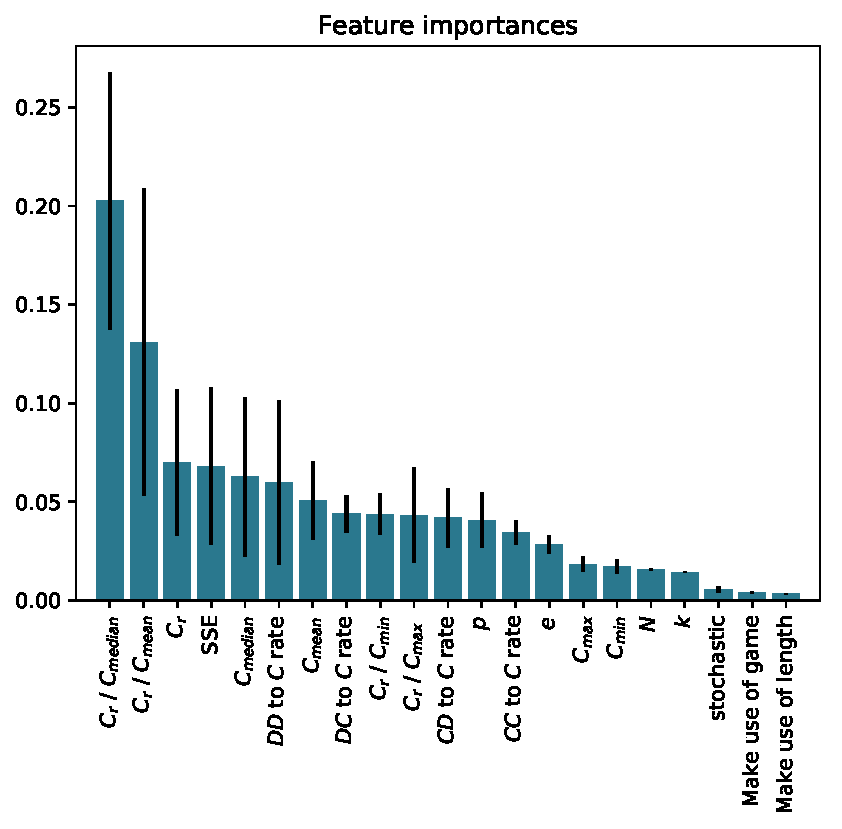
\includegraphics[width=.75\linewidth]{../k_means_output/probend_noise/_feature_importance_bar_plot.pdf}
        \end{center}
        \caption{Importance of features for clusters based on \(k\)means algorithm.}
    \end{subfigure}
    \caption{Importance of features in noisy probabilistic ending tournaments for different
    clustering methods.}\label{fig:clustering_importance_probend_noise}
\end{figure}

\begin{figure}[!htbp]
    \begin{subfigure}[t]{0.5\textwidth}
        \begin{center}
            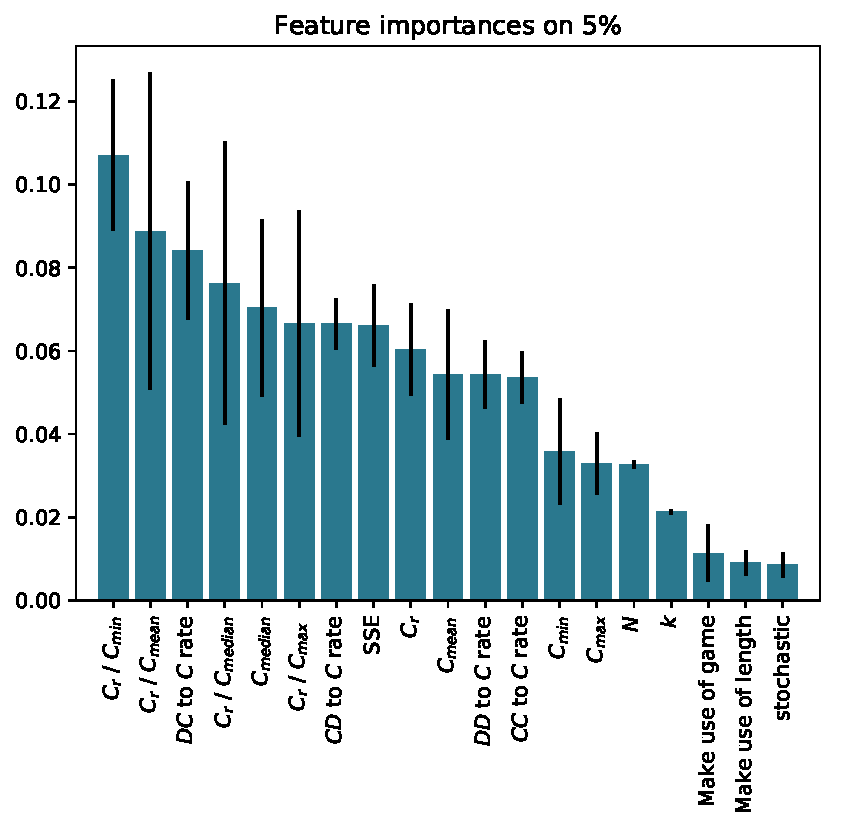
\includegraphics[width=.75\linewidth]{../new_output/merged/_feature_importance_bar_plot_cluster_on_0_05.pdf}
        \end{center}
        \caption{Importance of features for clusters on 5\% performance.}
    \end{subfigure}
    \begin{subfigure}[t]{0.5\textwidth}
        \begin{center}
            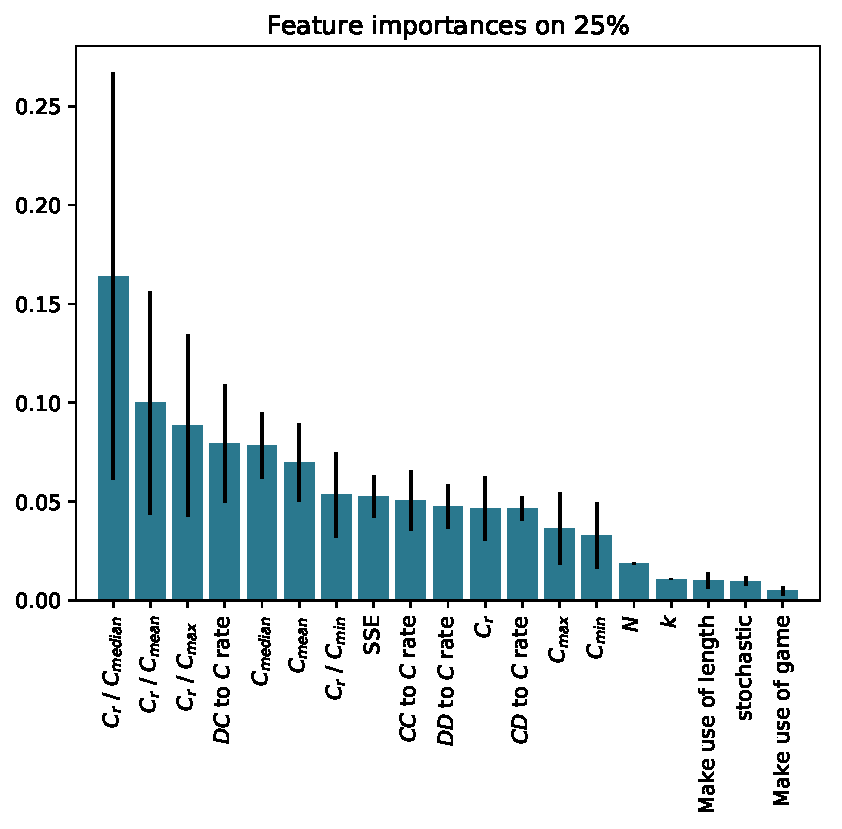
\includegraphics[width=.75\linewidth]{../new_output/merged/_feature_importance_bar_plot_cluster_on_0_25.pdf}
        \end{center}
        \caption{Importance of features for clusters on 25\% performance.}
    \end{subfigure}
    \begin{subfigure}[t]{0.5\textwidth}
        \begin{center}
            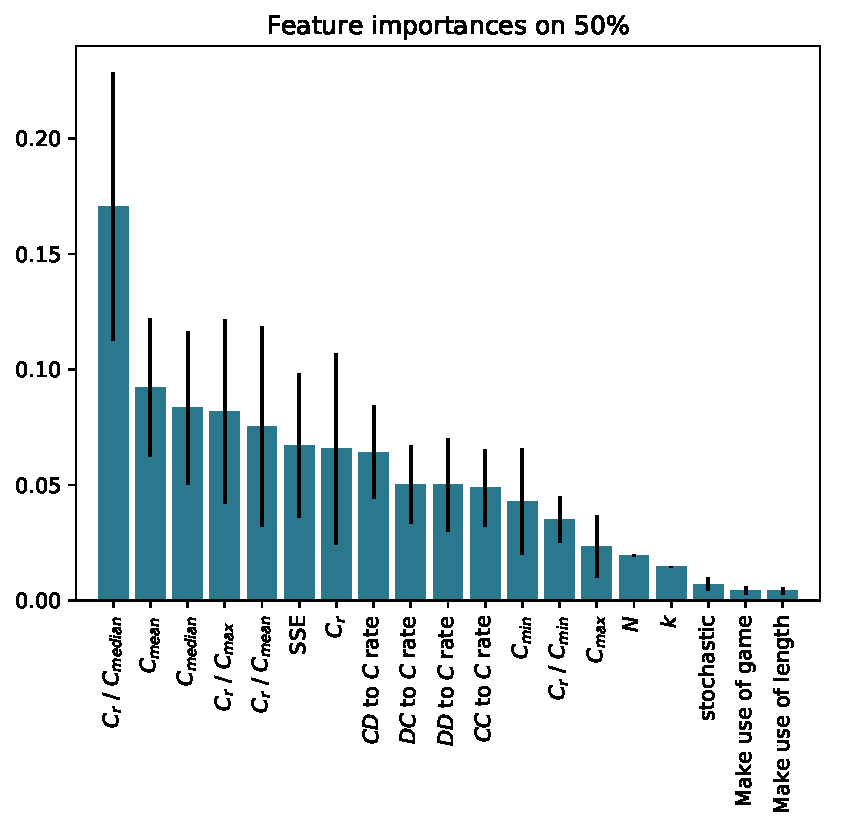
\includegraphics[width=.75\linewidth]{../new_output/merged/_feature_importance_bar_plot_cluster_on_0_5.pdf}
        \end{center}
        \caption{Importance of features for clusters on 50\% performance.}
    \end{subfigure}
    \begin{subfigure}[t]{0.5\textwidth}
        \begin{center}
            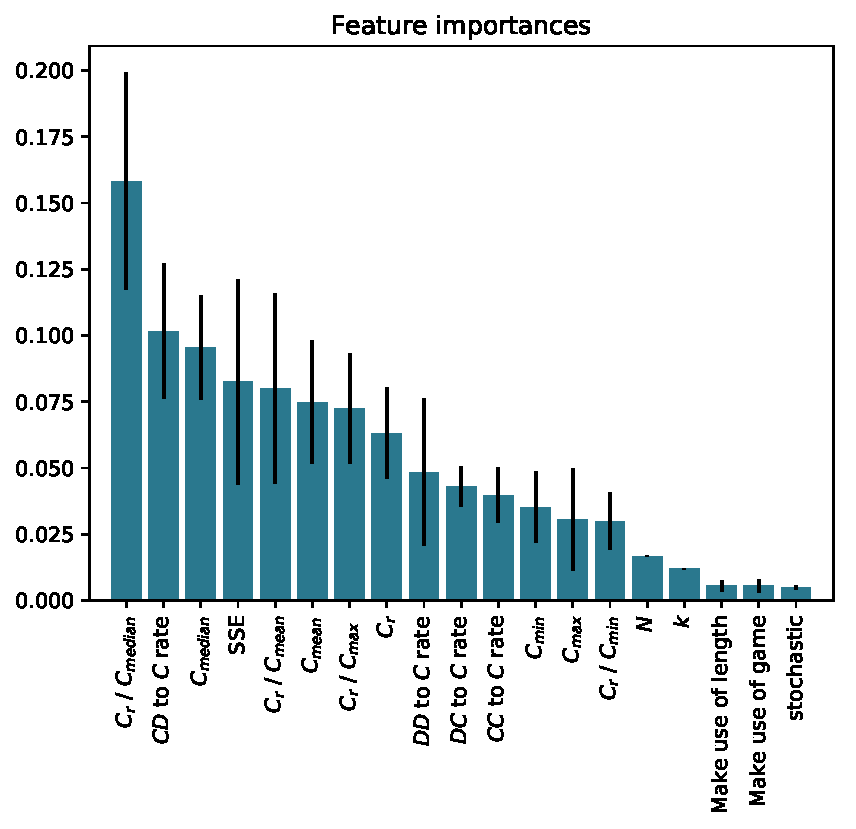
\includegraphics[width=.75\linewidth]{../k_means_output/merged/_feature_importance_bar_plot.pdf}
        \end{center}
        \caption{Importance of features for clusters based on \(k\)means algorithm.}
    \end{subfigure}
    \caption{Importance of features over all the tournaments for different
    clustering methods.}\label{fig:clustering_importance_overall}
\end{figure}
\section{Multivariate linear regression on median score}\label{app:regression_median_score}

A multivariate linear regression has also been fitted to model the relationship between
the features and the median score. The features included are given
by Table~\ref{table:linear_regression_on_median} alongside their corresponding \(p\) values
in the distinct tournaments and their regression coefficients.

\newcolumntype{g}{>{\columncolor{Gray}}c}
\begin{table}[h]
    \begin{center}
\resizebox{\textwidth}{!}{
\begin{tabular}{lggccggccgg}
    \toprule
    & \multicolumn{2}{g}{Standard} & \multicolumn{2}{c}{Noisy} & \multicolumn{2}{g}{Probabilistic ending} & \multicolumn{2}{c}{Noisy probabilistic ending} & \multicolumn{2}{g}{Overall}\\
    \midrule
    & \multicolumn{2}{g}{\(R\) adjusted: 0.576} & \multicolumn{2}{c}{\(R\) adjusted: 0.679} & \multicolumn{2}{g}{\(R\) adjusted: 0.816} & \multicolumn{2}{c}{\(R\) adjusted: 0.930} & \multicolumn{2}{g}{\(R\) adjusted: 0.318} \\
    {} &  Coefficient &  \(p\)-value &  Coefficient &  \(p\)-value &  Coefficient &  \(p\)-value &  Coefficient &  \(p\)-value &  Coefficient &  \(p\)-value \\
    \midrule
    $CC$ to $C$ rate   &  0.043 &  0.000 & -0.380 &  0.000 &  0.224 &  0.000 &  0.078 &    0.0 &  0.308 &    0.0 \\
    $CD$ to $C$ rate   & -0.325 &  0.000 &  0.124 &  0.000 &  0.060 &  0.000 &  0.073 &    0.0 & -0.014 &    0.0 \\
    $C_r$ / $C_{max}$  &      - &      - & -1.044 &  0.000 &      - &      - & -1.251 &    0.0 &      - &      - \\
    $C_r$ / $C_{mean}$ &  0.553 &  0.000 & -0.101 &  0.000 & -1.136 &  0.000 & -0.089 &    0.0 & -0.665 &    0.0 \\
    $C_{max}$          &  0.059 &  0.000 &      - &      - & -0.044 &  0.086 & -1.396 &    0.0 &      - &      - \\
    $C_{mean}$         &  1.837 &  0.000 &  3.078 &  0.000 &  1.506 &  0.000 &  3.645 &    0.0 &      - &      - \\
    $C_{min}$          &  0.156 &  0.000 &  1.528 &  0.000 &  0.311 &  0.000 &      - &      - &      - &      - \\
    $C_{min}$ / $C_r$  & -0.049 &  0.000 & -0.378 &  0.000 & -0.204 &  0.000 &      - &      - & -0.257 &    0.0 \\
    $DC$ to $C$ rate   & -0.204 &  0.000 &  0.074 &  0.000 &  0.066 &  0.000 &  0.066 &    0.0 &  0.007 &    0.0 \\
    $k$                & -0.000 &  0.853 & -0.000 &  0.987 &  0.000 &  0.008 &  0.000 &    0.0 &      - &      - \\
    $n$                & -0.000 &  0.000 &      - &      - &      - &      - &      - &      - &      - &      - \\
    $p_e$              &      - &      - &      - &      - &  0.025 &  0.000 & -0.095 &    0.0 &      - &      - \\
    $p_n$              &      - &      - &  0.124 &  0.000 &      - &      - &      - &      - &      - &      - \\
    SSE                & -0.294 &  0.000 & -0.319 &  0.000 &  0.055 &  0.000 &  0.010 &    0.0 & -0.015 &    0.0 \\
    constant           &  0.925 &  0.000 &  1.536 &  0.000 &  2.466 &  0.000 &  2.299 &    0.0 &  2.924 &    0.0 \\
    memory usage       &  0.010 &  0.000 & -0.004 &  0.000 &      - &      - &      - &      - &      - &      - \\
    \bottomrule
\end{tabular}}
\end{center}
\caption{Results of multivariate linear regressions with the median score as the dependent variable.
\(R\) squared is reported for each model.}
\label{table:linear_regression_on_median}
\end{table}
\section{List of strategies}\label{app:list_of_players}

The strategies used in this study which are from Axelrod-Python library version 3.0.0.

\begin{multicols}{3}
	\begin{enumerate}
		\item $\phi$~\cite{axelrodproject}
\item $\pi$~\cite{axelrodproject}
\item $e$~\cite{axelrodproject}
\item ALLCorALLD \cite{axelrodproject}
\item Adaptive~\cite{Li2011}
\item Adaptive Pavlov 2006~\cite{kendall2007iterated}
\item Adaptive Pavlov 2011~\cite{Li2011}
\item Adaptive Tit For Tat: 0.5~\cite{Tzafestas2000}
\item Aggravater~\cite{axelrodproject}
\item Alexei~\cite{lesswrong}
\item Alternator~\cite{Axelrod1981, Mittal2009}
\item Alternator Hunter~\cite{axelrodproject}
\item Anti Tit For Tat~\cite{Hilbe2013}
\item AntiCycler~\cite{axelrodproject}
\item Appeaser~\cite{axelrodproject}
\item Arrogant QLearner~\cite{axelrodproject}
\item Average Copier~\cite{axelrodproject}
\item Backstabber~\cite{axelrodproject}
\item Better and Better~\cite{prison}
\item Bully~\cite{Nachbar1992}
\item Calculator~\cite{prison}
\item Cautious QLearner~\cite{axelrodproject}
\item Champion~\cite{Axelrod1980b}
\item CollectiveStrategy~\cite{Li2009}
\item Contrite Tit For Tat~\cite{Axelrod1995}
\item Cooperator~\cite{Axelrod1981, Mittal2009, Press2012}
\item Cooperator Hunter~\cite{axelrodproject}
\item Cycle Hunter~\cite{axelrodproject}
\item Cycler CCCCCD~\cite{axelrodproject}
\item Cycler CCCD~\cite{axelrodproject}
\item Cycler CCCDCD~\cite{axelrodproject}
\item Cycler CCD~\cite{Mittal2009}
\item Cycler DC~\cite{axelrodproject}
\item Cycler DDC~\cite{Mittal2009}
\item DBS~\cite{Au2006}
\item Davis~\cite{Axelrod1980a}
\item Defector~\cite{Axelrod1981, Mittal2009, Press2012}
\item Defector Hunter~\cite{axelrodproject}
\item Double Crosser~\cite{axelrodproject}
\item Desperate \cite{Van2015}
\item DoubleResurrection~\cite{Eckhart2015}
\item Doubler~\cite{prison}
\item Dynamic Two Tits For Tat~\cite{axelrodproject}
\item EasyGo~\cite{Li2011, prison}
\item Eatherley~\cite{Axelrod1980b}
\item Eventual Cycle Hunter~\cite{axelrodproject}
\item Evolved ANN~\cite{axelrodproject}
\item Evolved ANN 5~\cite{axelrodproject}
\item Evolved ANN 5 Noise 05~\cite{axelrodproject}
\item Evolved FSM 16~\cite{axelrodproject}
\item Evolved FSM 16 Noise 05~\cite{axelrodproject}
\item Evolved FSM 4~\cite{axelrodproject}
\item Evolved HMM 5~\cite{axelrodproject}
\item EvolvedLookerUp1 1 1~\cite{axelrodproject}
\item EvolvedLookerUp2 2 2~\cite{axelrodproject}
\item Eugine Nier~\cite{lesswrong}
\item Feld~\cite{Axelrod1980a}
\item Firm But Fair~\cite{Frean1994}
\item Fool Me Forever~\cite{axelrodproject}
\item Fool Me Once~\cite{axelrodproject}
\item Forgetful Fool Me Once~\cite{axelrodproject}
\item Forgetful Grudger~\cite{axelrodproject}
\item Forgiver~\cite{axelrodproject}
\item Forgiving Tit For Tat~\cite{axelrodproject}
\item Fortress3~\cite{Ashlock2006}
\item Fortress4~\cite{Ashlock2006}
\item GTFT \cite{Gaudesi2016, Nowak1993}
\item General Soft Grudger~\cite{axelrodproject}
\item Gradual~\cite{Beaufils1997}
\item Gradual Killer~\cite{prison}
\item Grofman\cite{Axelrod1980a}
\item Grudger~\cite{Axelrod1980a, Banks1990, Beaufils1997, Van2015, Li2011}
\item GrudgerAlternator~\cite{prison}
\item Grumpy~\cite{axelrodproject}
\item Handshake~\cite{Robson1990}
\item Hard Go By Majority~\cite{Mittal2009}
\item Hard Go By Majority: 10~\cite{axelrodproject}
\item Hard Go By Majority: 20~\cite{axelrodproject}
\item Hard Go By Majority: 40~\cite{axelrodproject}
\item Hard Go By Majority: 5~\cite{axelrodproject}
\item Hard Prober~\cite{prison}
\item Hard Tit For 2 Tats~\cite{Stewart2012}
\item Hard Tit For Tat~\cite{PD2017}
\item Hesitant QLearner\cite{axelrodproject}
\item Hopeless~\cite{Van2015}
\item Inverse~\cite{axelrodproject}
\item Inverse Punisher~\cite{axelrodproject}
\item Joss~\cite{Axelrod1980a, Stewart2012}
\item Knowledgeable Worse and Worse~\cite{axelrodproject}
\item Level Punisher~\cite{Eckhart2015}
\item Limited Retaliate 2~\cite{axelrodproject}
\item Limited Retaliate 3~\cite{axelrodproject}
\item Limited Retaliate~\cite{axelrodproject}
\item MEM2~\cite{Li2014}
\item Math Constant Hunter~\cite{axelrodproject}
\item Meta Hunter Aggressive~\cite{axelrodproject}
\item Meta Hunter~\cite{axelrodproject}
\item Meta Majority~\cite{axelrodproject}
\item Meta Majority Finite Memory~\cite{axelrodproject}
\item Meta Majority Long Memory~\cite{axelrodproject}
\item Meta Majority Memory One~\cite{axelrodproject}
\item Meta Minority~\cite{axelrodproject}
\item Meta Mixer~\cite{axelrodproject}
\item Meta Winner~\cite{axelrodproject}
\item Meta Winner Deterministic~\cite{axelrodproject}
\item Meta Winner Ensemble~\cite{axelrodproject}
\item Meta Winner Finite Memory~\cite{axelrodproject}
\item Meta Winner Long Memory~\cite{axelrodproject}
\item Meta Winner Memory One~\cite{axelrodproject}
\item Meta Winner Stochastic~\cite{axelrodproject}
\item NMWE Deterministic~\cite{axelrodproject}
\item NMWE Finite Memory~\cite{axelrodproject}
\item NMWE Long Memory~\cite{axelrodproject}
\item NMWE Memory One~\cite{axelrodproject}
\item NMWE Stochastic~\cite{axelrodproject}
\item Naive Prober~\cite{Li2011}
\item Negation~\cite{PD2017}
\item Nice Average Copier~\cite{axelrodproject}
\item Nice Meta Winner~\cite{axelrodproject}
\item Nice Meta Winner Ensemble~\cite{axelrodproject}
\item Nydegger~\cite{Axelrod1980a}
\item Omega TFT~\cite{kendall2007iterated}
\item Once Bitten~\cite{axelrodproject}
\item Opposite Grudger~\cite{axelrodproject}
\item PSO Gambler 1 1 1~\cite{axelrodproject}
\item PSO Gambler 2 2 2~\cite{axelrodproject}
\item PSO Gambler 2 2 2 Noise 05~\cite{axelrodproject}
\item PSO Gambler Mem1 \cite{axelrodproject}
\item Predator~\cite{Ashlock2006}
\item Prober~\cite{Li2011}
\item Prober 2~\cite{prison}
\item Prober 3~\cite{prison}
\item Prober 4~\cite{prison}
\item Pun1~\cite{Ashlock2006}
\item Punisher~\cite{axelrodproject}
\item Raider~\cite{Ashlock2014}
\item Random Hunter~\cite{axelrodproject}
\item Random: 0.5~\cite{Axelrod1980a, Tzafestas2000}
\item Remorseful Prober~\cite{Li2011}
\item Resurrection~\cite{Eckhart2015}
\item Retaliate 2~\cite{axelrodproject}
\item Retaliate 3~\cite{axelrodproject}
\item Retaliate~\cite{axelrodproject}
\item Revised Downing~\cite{Axelrod1980a}
\item Ripoff~\cite{Ashlock2008}
\item Risky QLearner~\cite{axelrodproject}
\item SelfSteem~\cite{Andre2013}
\item ShortMem ~\cite{Andre2013}
\item Shubik~\cite{Axelrod1980a}
\item Slow Tit For Two Tats~\cite{axelrodproject}
\item Slow Tit For Two Tats 2~\cite{prison}
\item Sneaky Tit For Tat~\cite{axelrodproject}
\item Soft Go By Majority~\cite{Axelrod1981, Mittal2009}
\item Soft Go By Majority 10~\cite{axelrodproject}
\item Soft Go By Majority 20~\cite{axelrodproject}
\item Soft Go By Majority 40~\cite{axelrodproject}
\item Soft Go By Majority 5~\cite{axelrodproject}
\item Soft Grudger~\cite{Li2011}
\item Soft Joss~\cite{prison}
\item SolutionB1~\cite{Ashlock2015}
\item SolutionB5~\cite{Ashlock2015}
\item Spiteful Tit For Tat~\cite{prison}
\item Stalker~\cite{Carvalho2013}
\item Stein and Rapoport~\cite{Axelrod1980a}
\item Stochastic Cooperator~\cite{Adami2013}
\item Stochastic WSLS~\cite{axelrodproject}
\item Suspicious Tit For Tat~\cite{Beaufils1997, Hilbe2013}
\item TF1~\cite{axelrodproject}
\item TF2~\cite{axelrodproject}
\item TF3~\cite{axelrodproject}
\item Tester~\cite{Axelrod1980b}
\item ThueMorse~\cite{axelrodproject}
\item ThueMorseInverse~\cite{axelrodproject}
\item Thumper~\cite{Ashlock2008}
\item Tit For 2 Tats (\textbf{Tf2T})~\cite{Axelrod1981}
\item Tit For Tat (\textbf{TFT})~\cite{Axelrod1980a}
\item Tricky Cooperator~\cite{axelrodproject}
\item Tricky Defector~\cite{axelrodproject}
\item Tullock~\cite{Axelrod1980a}
\item Two Tits For Tat (\textbf{2TFT})~\cite{Axelrod1981}
\item VeryBad~\cite{Andre2013}
\item Willing \cite{Van2015}
\item Win-Shift Lose-Stay (\textbf{WShLSt})~\cite{Li2011}
\item Win-Stay Lose-Shift (\textbf{WSLS})~\cite{Kraines1989, Nowak1993, Stewart2012}
\item Winner12~\cite{mathieu2017}
\item Winner21~\cite{mathieu2017}
\item Worse and Worse\cite{prison}
\item Worse and Worse 2\cite{prison}
\item Worse and Worse 3\cite{prison}
\item ZD-Extort-2 v2~\cite{Kuhn2017}
\item ZD-Extort-2~\cite{Stewart2012}
\item ZD-Extort-4~\cite{axelrodproject}
\item ZD-GEN-2~\cite{Kuhn2017}
\item ZD-GTFT-2~\cite{Stewart2012}
\item ZD-SET-2~\cite{Kuhn2017}
	\end{enumerate}
\end{multicols}

\bibliographystyle{plain}
\bibliography{bibliography}

\end{document}